% Weight-Dictionary Decomposition, ICLR 2027 submission (derived from wdd_tmlr.tex by tools/derive.py)
\documentclass{article}
\usepackage{iclr2027_conference,times}
% \iclrfinalcopy  % camera-ready only

\usepackage[utf8]{inputenc}
\usepackage[T1]{fontenc}
\usepackage{hyperref}
\usepackage{url}
\usepackage{booktabs}
\usepackage{amsfonts,amsmath}
\usepackage{microtype}
\usepackage{enumitem}
\usepackage{longtable}
\usepackage{float}
\usepackage{adjustbox}
\usepackage{pgfplots}
\pgfplotsset{compat=1.17}
\raggedbottom
\setlength{\abovecaptionskip}{5pt}
\setlength{\belowcaptionskip}{2pt}

\title{Weight-Dictionary Decomposition: Reading a Transformer's Residual Stream with Its Own Writes}

\author{Anonymous authors}

\begin{document}

\maketitle

\begin{abstract}
Sparse autoencoders interpret the residual states of a transformer through an overcomplete dictionary trained on activations. We build the dictionary from the weights instead. Each component's write into the residual stream is confined to a direction or subspace that its weights fix in advance, so collecting those directions from the checkpoint yields an overcomplete, training-free dictionary in which each atom is labeled with the component that wrote it. Weight-dictionary decomposition (WDD) sparse-codes an observed state over this dictionary to infer its largest native writes and their strengths. We score it against exact ground truth from hooked forward passes in eight models from six families, up to 7B parameters, on two corpora. An identified write has the right sign in more than 99.7\% of cases in all eight models. Its magnitude is recovered with a median relative error between 0.25 and 0.54 in seven of them, biased upward for small writes because a 64-atom support absorbs the writes it leaves out, and it is not recovered in Pythia-6.9B. The identification rate rises with scale to 0.98 for Llama-7B. The rest of the support is not a list of writers, since only a quarter to seven tenths of the MLP atoms it selects are real writes at that token. Identification is bounded by an observability ceiling that we measure in all eight models. Once the other writes cancel a write along its own direction, OMP no longer finds it at the tested budget, although a probe on the full state shows that the information usually survives the cancellation. Used as measurement axes, the write directions single out a GPT-2 neuron that appears to erase the model's massive activation channel, and interventions under a frozen-normalization control reinterpret it as a participant in maintaining that channel, one that a distributed suppression field keeps below its clean level. In pre-specified comparisons at thirty nominees per arm, WDD beats a marginal outlier screen at nominating live circuits but does not outperform a correlation screen, and we argue that its distinctive contribution is the mechanistic content that each nomination carries.
\end{abstract}

\section{Introduction}
\label{sec:intro}

Interpreting the residual stream of a transformer currently runs through trained sparse dictionaries. Sparse autoencoders (SAEs) learn an overcomplete basis, whose elements are conventionally called \emph{atoms}, from millions of activation samples \citep{bricken2023,cunningham2023}. The training is the expense, and the learned atoms are the interpretive risk, because a direction that reconstructs activations well need not correspond to anything the model actually does.

A structural fact suggests an alternative. As the circuits literature established \citep{elhage2021}, the residual stream is a sum of writes through fixed weight matrices, so each component's write is confined in advance to a direction or subspace that its weights determine. An MLP neuron writes along one fixed direction with an input-dependent coefficient, an attention head writes inside the row space of its output projection, and the embedding writes along fixed vectors. Prior work interprets these weight vectors directly \citep{geva2021,dar2022,peng2025} or tracks a known write forward through the stream \citep{janiak2023}. To our knowledge, no prior method inverts the relationship by asking, given one observed state and the checkpoint, which native writes are most consistent with that state and at what strength.

We evaluate this inversion both as an instrument, scored on exact ground truth from hooked forward passes, and as a discovery tool whose hypotheses we then test by intervention. We make three contributions.
\begin{enumerate}[leftmargin=*,nosep]
\item \textbf{A training-free, provenance-bearing dictionary, validated as an instrument.} With no training at all, the dictionary reconstructs the massive-activation states almost exactly and the typical states better than the sampled rotations of itself at all tested budgets, and the rotation control shows that overcompleteness alone does not explain the advantage. Attribution splits into identification, which is capped by a measurable observability ceiling, and estimation, which recovers the sign of a write throughout and its magnitude with a bias that we measure decile by decile, while the support beyond the largest writes is mostly spurious, which we quantify. Both findings replicate across eight models from six families, up to 7B parameters, and on a second corpus, with bootstrap intervals on each headline number.
\item \textbf{A discovery pipeline with intervention discipline.} A null-tested taxonomy of write roles nominates a GPT-2 neuron whose apparent erasure of the massive activation channel resolves, under intervention, into participation in maintaining that channel, with a suppression field that holds back a reserve bank of later neurons.
\item \textbf{Pre-specified nomination comparisons, reported in full.} WDD beats a marginal outlier screen on causal response but does not outperform a one-line correlation baseline on either tier. We argue that its advantage is representational, since each nomination carries a native write direction, a predicted partner, and a falsifiable role hypothesis.
\end{enumerate}

\section{Method}
\label{sec:method}

\paragraph{Dictionary.} Consider an MLP neuron $j$ with down-projection row $\mathbf{w}_j$ and post-nonlinearity activation $a_j$, which adds $a_j\mathbf{w}_j$ to the residual stream. We factor this write into a fixed unit direction and an input-dependent coefficient,
\begin{equation}
a_j\mathbf{w}_j = c_j\,\mathbf{d}_j, \qquad
\mathbf{d}_j=\frac{\mathbf{w}_j}{\lVert\mathbf{w}_j\rVert}, \qquad
c_j=a_j\lVert\mathbf{w}_j\rVert ,
\label{eq:write}
\end{equation}
so that the direction is a property of the checkpoint and only the coefficient depends on the input. We collect unit-normed atoms for each model-native direction whose write can reach the target state. These are the token and position embedding rows, which enter before block 0, an SVD basis of the row space of each attention head's output projection, which is the subspace that head's write can occupy, the MLP down-projection rows, and the two output biases of each block. Each atom carries a deterministic label giving its block, its component and its write subspace. MLP atoms correspond one to one with neuron write directions, whereas attention atoms span a head's attainable subspace and are not individual causal writes. For GPT-2 small at layer 6, which collects blocks 0 to 6, the dictionary has $m=78{,}175$ atoms in $d=768$ dimensions, about 102 times overcomplete. GPT-2 stores its projections in Conv1D form, whose rows are the write directions. Where the down-projection is a standard linear layer, its columns play that role instead, and gating changes only the coefficients.

\paragraph{Inverse problem.} Given an observed state $\mathbf{x}$ and the dictionary $D=[\mathbf{d}_1\cdots\mathbf{d}_m]$, WDD estimates a sparse coefficient vector by orthogonal matching pursuit with $k$ active atoms,
\begin{equation}
\hat{\mathbf{c}}=\mathrm{OMP}_k(D,\mathbf{x}), \qquad \mathbf{x}\approx D\hat{\mathbf{c}},
\label{eq:omp}
\end{equation}
and we read each $\hat c_i$ as the inferred write of the component that atom $i$ belongs to. All control dictionaries in this paper run through the identical OMP code at the identical size. A second mode, \emph{one-shot ranking}, keeps the $k$ atoms most correlated with $\mathbf{x}$ without orthogonalization and then refits on that support. It is the projection reading that OMP's explaining-away refines, and Section~\ref{sec:attrib} uses both for identification.

\paragraph{Survival and write roles.} For a write with unit direction $\mathbf{d}$ and signed coefficient $c$, we define its survival in a later state $\mathbf{x}$ as the fraction of the write that is still present along its own direction,
\begin{equation}
s=\frac{\mathbf{x}\cdot\mathbf{d}}{c},
\label{eq:surv}
\end{equation}
which is the projection ratio of \citet{janiak2023}. Evaluating survival at the moment of writing, where $\mathbf{x}_{\text{pre}}$ is the state the write was added to, gives the birth survival
\begin{equation}
s_{\text{birth}}=1+\frac{\mathbf{x}_{\text{pre}}\cdot\mathbf{d}}{c},
\label{eq:birth}
\end{equation}
which classifies a write's role by what it did to the content already present along its direction. We call a write \emph{reinforcing} when $s_{\text{birth}}>1$, \emph{novel} when $s_{\text{birth}}$ lies within 0.5 of 1, and \emph{counter-aligned} when $s_{\text{birth}}<0$, in which case it opposed existing content. These labels record what a component wrote relative to the state, and we stress that assigning a mechanism requires intervention.

\section{Experimental Setup}
\label{sec:setup}

Our primary model is GPT-2 small, and we decompose the state after block 6, the middle of its twelve blocks, over 32{,}768 held-out WikiText-2 tokens, on which the model's clean cross-entropy is 3.647. We chose the middle of the stack because our questions need both sides of it. Seven blocks of writers precede the state, so attribution has a large population to identify, and five blocks of computation follow it, so cancellation can be measured. To check that the choice is not special we repeated the reconstruction after block 8 and found the same picture, a typical-state FVU of 0.349 against 0.338 at $k=32$ (Appendix~\ref{app:recon}). We run OMP to $k=64$ atoms and read the support at $k=32$ and $k=64$, which brackets the sparsity of a trained SAE at this layer (Appendix~\ref{app:z4}), and Appendices~\ref{app:recon} and~\ref{app:z5} sweep $k$ from 4 to 256.

We use train-split tokens for the centering means and for the data-based controls, so that no evaluation token enters a dictionary or a control. The one exception, stated in Appendix~\ref{app:ci}, is that the GPT-2 attribution runs center on the evaluation mean. Centering also settles what the decomposition estimates. It subtracts one fixed vector from all states, so its target is the raw ledger coefficient shifted by that vector's component along the atom, the same offset at each token. We leave the ledger coefficients raw and count the offset as part of the estimation error we report. For the families other than GPT-2 the dictionary carries no bias atoms, so each block's output bias, a fixed vector, is absorbed into the centering in the same way.

To learn whether anything we find is particular to GPT-2, we rebuild the dictionary at the middle layer of SmolLM2-135M, Qwen2.5-0.5B, Pythia-410m and OLMo-1B, and again at 7B scale for Qwen2.5-7B, Llama-7B and Pythia-6.9B. The eight models span gated and non-gated MLPs, learned and rotary positions, and 124M to 7B parameters, and we repeat the whole sweep on a Pile-derived corpus. The oracle baselines of Section~\ref{sec:attrib} use samples of 16{,}384 tokens. The sweep of Section~\ref{sec:families} evaluates 32{,}768 states per model and corpus under one protocol, and its intervals come from a bootstrap over the 64 evaluation sequences. Runs of the individual experiment scripts on 8{,}192 states agree with it to within 0.001 in FVU, 0.021 in recall and 0.017 in $r$ (Appendix~\ref{app:ci}).

One convention matters for all reconstruction numbers, and we arrived at it by asking where the variance of a residual state is concentrated. In each model, one to four states per sequence, its first and sometimes one or two of the next few, have a norm above ten times the median, and nothing lies between five and ten times the median in any of the sixteen model and corpus pairs. These are the attention-sink states of the massive-activation literature \citep{sun2024}. They carry between 59\% and 99\% of the summed variance, and any dictionary that contains the massive-channel directions reconstructs them from a few atoms, so an FVU over all states mostly measures them. We report FVU over the \emph{typical} states, the other 99.4\% or more, and give the sink states separately. Our ground truth is the \emph{ledger}, which records each MLP neuron's true coefficient $c_j$ of Equation~\ref{eq:write} from hooked forward passes. Since attention writes carry no per-component scalar, we score attribution on MLP writes, and we call a token's \emph{dominant writes} its top-3 ledger entries by magnitude.

\section{Results}
\label{sec:results}

\subsection{Reconstruction Is Not Attribution}
\label{sec:recon}

\begin{figure}[t]
\centering
\begin{minipage}[t]{0.49\linewidth}
\centering
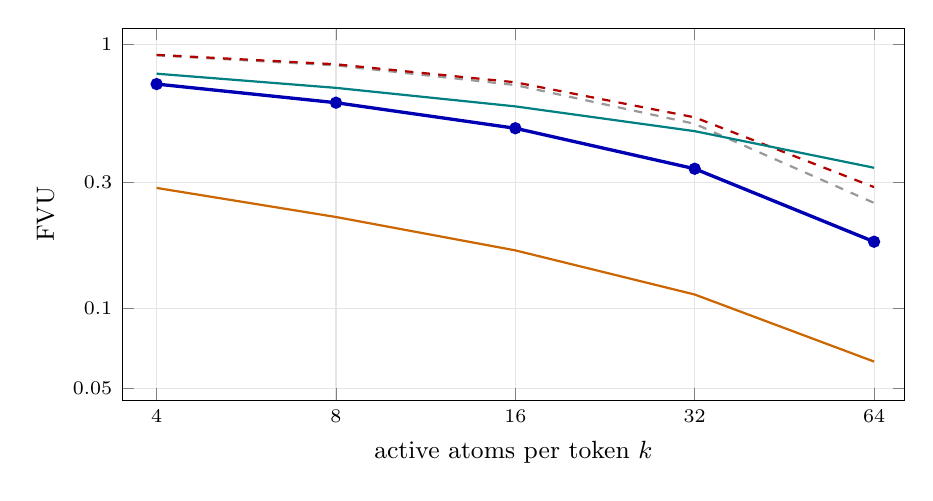
\begin{tikzpicture}
\begin{axis}[
  width=0.95\linewidth, height=0.52\linewidth,
  xmode=log, ymode=log, log ticks with fixed point, xmin=3.5, xmax=72, ymin=0.045, ymax=1.15, clip=false,
  xlabel={active atoms per token $k$}, ylabel={FVU},
  xtick={4,8,16,32,64}, xticklabels={4,8,16,32,64},
  ytick={0.05,0.1,0.3,1}, yticklabels={0.05,0.1,0.3,1},
  tick label style={font=\scriptsize}, label style={font=\small},
  grid=major, grid style={black!10}]
% FIG1-BEGIN (regenerated by tools/fig1.py from exp_a_tokens.npz and exp_d_tokens.npz; do not edit by hand)
\addplot[thick, color=black!40, dashed] coordinates
  {(4,0.908)(8,0.832)(16,0.701)(32,0.500)(64,0.251)};
\addplot[thick, color=red!70!black, dashed] coordinates
  {(4,0.912)(8,0.840)(16,0.718)(32,0.529)(64,0.288)};
\addplot[thick, color=teal] coordinates
  {(4,0.774)(8,0.684)(16,0.582)(32,0.469)(64,0.341)};
\addplot[very thick, color=blue!70!black, mark=*, mark size=1.6pt] coordinates
  {(4,0.707)(8,0.601)(16,0.481)(32,0.338)(64,0.179)};
\addplot[thick, color=orange!80!black] coordinates
  {(4,0.286)(8,0.222)(16,0.166)(32,0.113)(64,0.063)};
% FIG1-END
\end{axis}
\end{tikzpicture}
\end{minipage}\hfill
\begin{minipage}[t]{0.49\linewidth}
\centering
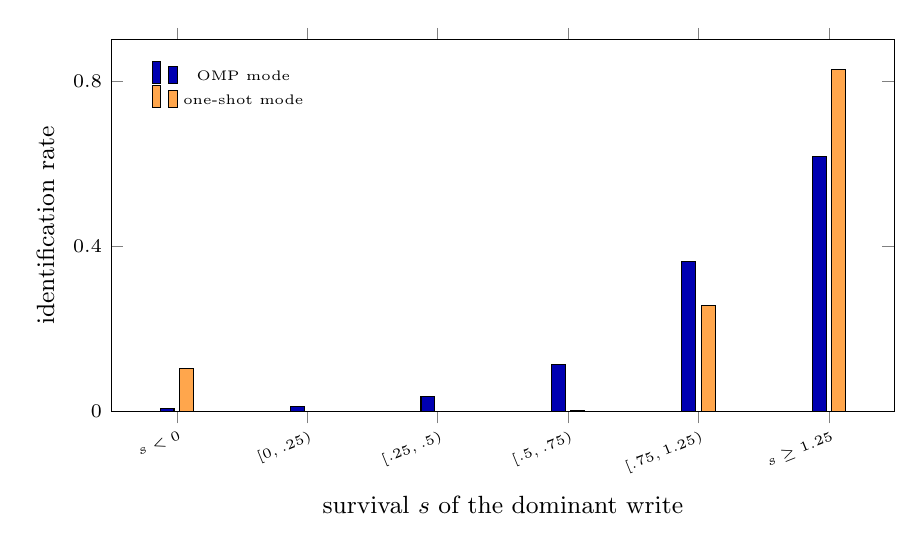
\begin{tikzpicture}
\begin{axis}[
  width=0.95\linewidth, height=0.52\linewidth,
  ybar, bar width=5pt, enlarge x limits=0.1,
  xtick={1,2,3,4,5,6},
  xticklabels={{$s<0$},{$[0,.25)$},{$[.25,.5)$},{$[.5,.75)$},{$[.75,1.25)$},{$s\ge1.25$}},
  x tick label style={font=\tiny, rotate=22, anchor=north east, xshift=3pt, yshift=1pt},
  xlabel={survival $s$ of the dominant write}, ylabel style={font=\scriptsize},
  ylabel={identification rate}, ymin=0, ymax=0.9, ytick={0,0.4,0.8},
  legend style={font=\tiny, at={(0.04,0.96)}, anchor=north west, draw=none, fill=none, row sep=-2pt},
  tick label style={font=\scriptsize}, label style={font=\small}]
\addplot[fill=blue!70!black] coordinates
  {(1,0.007) (2,0.012) (3,0.036) (4,0.114) (5,0.364) (6,0.618)};
\addlegendentry{OMP mode}
\addplot[fill=orange!70] coordinates
  {(1,0.104) (2,0.000) (3,0.000) (4,0.003) (5,0.257) (6,0.829)};
\addlegendentry{one-shot mode}
\end{axis}
\end{tikzpicture}
\end{minipage}
\par\vspace{2pt}\centering{\tiny
\tikz[baseline=-0.5ex]\draw[thick, color=black!40, dashed] (0,0)--(1.4em,0); random\hspace{1.4em}
\tikz[baseline=-0.5ex]\draw[thick, color=red!70!black, dashed] (0,0)--(1.4em,0); rotated weight dictionary\hspace{1.4em}
\tikz[baseline=-0.5ex]\draw[thick, color=teal] (0,0)--(1.4em,0); PCA, best $k$ per state\hspace{1.4em}
\tikz[baseline=-0.5ex]\draw[very thick, color=blue!70!black] (0,0)--(1.4em,0); \textbf{weight dictionary}\hspace{1.4em}
\tikz[baseline=-0.5ex]\draw[thick, color=orange!80!black] (0,0)--(1.4em,0); sampled activations\par}
\caption{\textbf{Left:} reconstruction of the typical GPT-2 layer-6 states as a function of sparsity. The 64 sink states, 80\% of the variance, are reconstructed by the weight dictionary at an FVU below 0.001 and by its rotation near 0.5. One Gram-preserving rotation of the atoms moves the weight dictionary to the random floor. The matched comparison with a trained SAE is in Appendix~\ref{app:z4}. \textbf{Right:} identification rate of each token's dominant writes, binned by their survival $s$ in the layer-6 state. Under OMP, writes whose direction has been cancelled, those with $s<0.25$, are identified in about 1\% of cases, against 62\% for reinforced writes with $s\ge1.25$, while one-shot ranking identifies 83\% of reinforced writes and 10\% of counter-aligned ones.}
\label{fig:fvu}
\end{figure}

We began with the plainest question, whether a dictionary that nobody trained can reconstruct a residual state at all. The left panel of Figure~\ref{fig:fvu} sweeps sparsity on the typical states. With no training, the dictionary falls between PCA and a dictionary of sampled activations at each $k$. At $k=32$ it reaches an FVU of 0.338, against 0.469 for PCA and 0.113 for the sampled dictionary, and at $k=64$ it reaches 0.179. The 64 sink states, which carry 80\% of the variance, it reconstructs at an FVU of 0.0003, and splicing its $k=64$ reconstruction back into the forward pass raises cross-entropy by 0.178. The next question was where that reconstruction comes from, the overcompleteness of the dictionary or its alignment with the model's coordinates. Applying one Gram-preserving rotation to all atoms keeps all pairwise angles and destroys the alignment. It moves reconstruction to the random floor, 0.529 against 0.500 at $k=32$ on the typical states and 0.55 on the sink states. Overcompleteness alone does not explain the advantage, and alignment with the model's residual coordinate system does. The figure does not depend on the seed. Three rotations drawn from three seeds, in this control, in the re-implementation of Appendix~\ref{app:audit} and in the sweep of Appendix~\ref{app:ci}, give all-state FVU 0.549, 0.517 and 0.531 at $k=32$, against 0.501 to 0.507 for random directions.

A trained SAE is the natural comparison, and we wanted it on identical states rather than on borrowed numbers (Appendix~\ref{app:z4}). The residual-stream SAE of \citet{bloom2024} for this layer was trained on OpenWebText with 128-token contexts, and when we ran it on our 512-token states it failed past the positions it saw in training, so we compared in its own regime instead. On 32{,}768 OpenWebText states it activates 59 features per state on average and reaches an FVU of 0.121 with a cross-entropy cost of 0.155. At the same sparsity the training-free dictionary reaches 0.187 and 0.172, and at $k=64$ it reaches 0.169 and 0.146. The trained dictionary leaves 0.121 of the variance unexplained where ours leaves 0.187 at matched sparsity, the two are close in what the forward pass loses, and each atom of ours is labeled with its writer, which no SAE feature is.

That label is the reason to build the dictionary this way, and it led us to the control we consider the most important negative result of the section. If reconstruction quality reflected provenance, a dictionary that could not have written the state should reconstruct it badly. We drew the block atoms of a dictionary only from blocks 7 to 11, so that none of them could have contributed to the state, and kept the embedding rows, which make up 73\% of both dictionaries and can contribute. It still reaches FVU 0.449 at $k=32$, against 0.358 for a correct dictionary subsampled to the same size and 0.529 for the rotation, and it reconstructs the sink states as exactly as the correct dictionary does. We then removed the embedding rows from both dictionaries to rule them out, and nothing changed. Block atoms of blocks 7 to 11 alone reach 0.490 at $k=32$ on the typical states, against 0.375 for the correct block atoms subsampled to the same size and 0.561 for their rotation (Appendix~\ref{app:d2}). Low FVU cannot validate provenance. The provenance of a dictionary vector is known by construction, but whether a recovered coefficient belongs to that writer is a separate question, so from here on we score it directly against the ledger.

\subsection{Attribution and the Observability Ceiling}
\label{sec:attrib}

The ledger lets us ask what reconstruction could not answer, whether the atoms OMP selects are the writes that produced the state. A token's largest true write appears in the $k=64$ OMP support 64.7\% of the time, rising from 40\% in the lowest magnitude decile of that write to 96\% in the highest (Appendix~\ref{app:recall-decile}). One-shot ranking, the second mode of Section~\ref{sec:method}, does better at 76.6\%, because the orthogonalization in OMP explains away correlated true writers once the state is nearly reconstructed. When a dominant write is identified, the next question is how well its coefficient is estimated. Its sign is recovered in 99.8\% of cases and its magnitude with a median relative error of 0.44, over-estimated by a median factor of 1.66 in the smallest magnitude decile and 1.45 in the largest, because the 64-atom support absorbs the writes it leaves out. A correlation is the obvious summary of this, and here it misleads. Between recovered and true coefficients it is 0.998 over all states but 0.58 over the typical states, because the 0.13\% of identified writes at the sink states span a range of magnitudes that dominates the statistic. Even on the typical states the within-decile correlation is below 0.28 in all magnitude deciles but the top one. We report the calibration instead and keep the correlations in Appendix~\ref{app:ci}.

Why does identification stop at 65\%? We ruled out two causes first. It is not atom duplication, because clustering near-duplicate atoms moves recall only from 0.647 to 0.664, and it is not write age, which predicts identification at a chance-level AUC of 0.51. It is observability, as the right panel of Figure~\ref{fig:fvu} shows, and given the ledger coefficient WDD can certify that a direction has been cancelled. To locate the failure we built two oracle baselines. On synthetic states built purely from each token's MLP writes, recall is essentially unchanged at 0.62 for OMP and 0.67 for one-shot ranking, so the ceiling belongs to the geometry of the writes themselves. The other native writes cancel a component along its own direction, whether they came before it or after it, and OMP does not recover it. Refitting on the true top-3 atoms alone yields an aggregate $r$ of 0.55 over all dominant writes and 0.13 on erased ones, against 0.998 for the full support on the identified ones. On the same identified typical-state cases the refit reaches a median relative error of 0.68 where the full support reaches 0.44 (Appendix~\ref{app:z6}). The joint estimation over the full support recovers the coefficients somewhat better than the true atoms alone in five of the eight models, and no better in OLMo-1B and Qwen2.5-7B.

The full support then raised its own question. If OMP finds the largest writes, what are the other sixty atoms? On the typical states, MLP atoms make up 62\% of GPT-2's 64-atom support, and only 35\% of those are real writes at that token, meaning writes whose ledger coefficient is at least 5\% of the token's largest. The other 65\% are spurious, they carry 57\% of the recovered MLP coefficient mass, and the real atoms beyond the three dominant writes are over-estimated by a median factor of 2.1 (Appendix~\ref{app:z6}). OMP finds the largest writes and signs them, and it fills the rest of the support with atoms that explain the residual without corresponding to writes, so the support is not a list of writers. Across the eight models the real share of the selected MLP atoms runs from 24\% for SmolLM2 to 71\% for Llama-7B, and the spurious share of the coefficient mass from 25\% to 68\%.

Cancellation is directional, however, and we wanted to know whether the information is gone or only moved. A leakage-controlled ridge probe on the full state recovers the activations of the lowest-survival writers of block 3 at a median out-of-sample $R^2$ of 0.40, against 0.59 for intact writers, while their own direction carries none, and injected atoms are recovered again at a slope of 0.90. The information survives, and the ceiling is a property of OMP and the dictionary at the tested budget, not of the state. Full tables are in Appendix~\ref{app:attrib}.

\subsection{Generality}
\label{sec:families}

\begin{table}[t]
\centering\footnotesize\setlength{\tabcolsep}{4pt}\renewcommand{\arraystretch}{0.92}
% TABLE1-BEGIN (regenerated by tools/splice_table1.py from exp_z2_ci.json; do not edit by hand)
\caption{Eight models at their middle layers on WikiText-2, one protocol throughout: 32{,}768 evaluation states per model, brackets are 95\% bootstrap intervals over the 64 evaluation sequences. FVU is over the typical states. The one to four sink states per sequence, whose norm exceeds ten times the median, carry the stated share of the variance and the weight dictionary reconstructs them almost exactly, so their FVU at $k=32$ is listed separately as weight / rotated. Recall is OMP-mode top-1 identification of each token's largest write. The last three columns describe the identified dominant writes on typical states: the share whose sign is recovered, the median relative error of the recovered coefficient, and the median ratio of recovered to true coefficient in the smallest and the largest magnitude decile. The 7B-class rows were run in bfloat16 (float32 control in Appendix~\ref{app:fp32}).}
\label{tab:families}
\begin{adjustbox}{max width=\linewidth}
\begin{tabular}{lcccccccccc}
\toprule
Model & FVU at $k=32$ & at $k=64$ & rotated, $k=32$ & sink share & sink FVU & top-1 recall & sign & median rel. error & ratio, deciles 1 / 10 \\
\midrule
GPT-2 small, 124M & 0.338 [0.337, 0.340] & 0.179 & 0.529 & 80\% & 0.0003 / 0.53 & 0.647 [0.637, 0.657] & 99.8\% & 0.44 [0.44, 0.45] & 1.66 / 1.45 \\
SmolLM2-135M & 0.269 [0.268, 0.270] & 0.113 & 0.421 & 98\% & 0.0005 / 0.42 & 0.670 [0.661, 0.680] & 100.0\% & 0.54 [0.53, 0.54] & 1.97 / 0.73 \\
Qwen2.5-0.5B & 0.408 [0.407, 0.408] & 0.219 & 0.527 & 96\% & 0.0013 / 0.52 & 0.459 [0.451, 0.467] & 100.0\% & 0.46 [0.45, 0.46] & 1.58 / 0.43 \\
Pythia-410m & 0.503 [0.502, 0.504] & 0.303 & 0.592 & 91\% & 0.0037 / 0.59 & 0.481 [0.472, 0.490] & 99.9\% & 0.41 [0.40, 0.42] & 1.75 / 1.04 \\
OLMo-1B & 0.563 [0.561, 0.564] & 0.435 & 0.773 & 97\% & 0.0006 / 0.78 & 0.693 [0.687, 0.699] & 99.7\% & 0.34 [0.34, 0.34] & 1.06 / 0.51 \\
\midrule
Qwen2.5-7B & 0.555 [0.551, 0.558] & 0.459 & 0.847 & 99\% & 0.0039 / 0.84 & 0.673 [0.663, 0.685] & 100.0\% & 0.50 [0.50, 0.51] & 0.97 / 0.29 \\
Llama-7B & 0.631 [0.628, 0.633] & 0.533 & 0.872 & 86\% & 0.0002 / 0.87 & 0.981 [0.979, 0.983] & 100.0\% & 0.25 [0.25, 0.25] & 1.39 / 1.17 \\
Pythia-6.9B & 0.711 [0.709, 0.713] & 0.610 & 0.868 & 59\% & 0.0270 / 0.87 & 0.787 [0.779, 0.795] & 100.0\% & 1.03 [1.02, 1.04] & 2.19 / 1.86 \\
\bottomrule
\end{tabular}
\end{adjustbox}
% TABLE1-END
\end{table}

Estimation follows one pattern in all eight models rather than an architectural divide. The sign of an identified write is recovered in at least 99.7\% of cases, which is informative for the gated-MLP families, where half of the dominant writes are negative, and trivial for GPT-2 and Pythia, whose GELU coefficients are almost all positive. The magnitudes are biased in the same direction everywhere. Small writes are over-estimated in all eight models, by a median factor between 1.1 and 2.0 in the lowest magnitude decile, because a 64-atom support absorbs the writes it leaves out. The largest writes are under-estimated in the gated families except Llama-7B, by a factor of 0.4 to 0.7 in the top decile. The median relative error of an identified coefficient is 0.44 for GPT-2, 0.41 for Pythia-410m, 0.46 for Qwen2.5-0.5B, 0.54 for SmolLM2 and 0.34 for OLMo-1B. A correlation would hide all of this. In the gated families the signed correlation within a magnitude decile is 0.88 or more because it records the sign, and across deciles it is 0.99 because it records the range of magnitudes, so we report the calibration and keep the correlations in Appendix~\ref{app:ci}.

We also asked whether the reconstruction advantage is confined to the massive channels. They dominate the all-state variance, with the five highest-variance coordinates carrying between 91\% and 98\% of it across the four sub-1B families, yet off those five coordinates the dictionary still reaches an FVU between 0.34 and 0.60 on the typical states, where its rotation reaches between 0.49 and 0.79. The whole sweep replicates on a Pile sample (Appendix~\ref{app:ci}). For GPT-2 the typical-state FVU at $k=32$ is 0.358 [0.354, 0.362] against 0.530 rotated, with a top-1 recall of 0.568 [0.546, 0.588]. Across the eight models the largest changes between the corpora are 0.08 in recall, for GPT-2, 0.06 in FVU, for OLMo-1B, and 0.07 in the median relative error, for GPT-2.

Three 7B-class models, which occupy the lower rows of Table~\ref{tab:families}, extend the sweep by an order of magnitude in parameters, and the first thing we looked for was whether the rotation gap changes with scale. At 7B the rotation is again indistinguishable from random, with both between FVU 0.85 and 0.87 at $k=32$ on typical states, while the dictionary reaches 0.555 for Qwen2.5-7B, 0.631 for Llama-7B and 0.711 for Pythia-6.9B. The sink states carry 99\%, 86\% and 59\% of the variance in that order, and the dictionary reconstructs them at an FVU below 0.03 where the rotation stays above 0.84. The advantage at a fixed budget of 32 atoms is a factor of 1.2 to 1.6 in all eight models and does not widen with scale. The typical-state FVU itself rises with width, and we suspected a budget effect, since 32 atoms cover a smaller fraction of a wider space. Matching the budget to the width confirms it. At $k=d/16$ the dictionary reaches between 0.21 and 0.30 in all eight models and its rotation between 0.33 and 0.39, and at $k=d/12$ it reaches between 0.15 and 0.22 against 0.23 and 0.29. Models from 124M to 7B parameters reconstruct alike at the same fraction of their dimension, and alignment gives a factor of 1.2 to 1.7 at each scale (Appendix~\ref{app:z5}). Off the five highest-variance coordinates the dictionary reaches 0.68, 0.66 and 0.74 where the rotation reaches 0.88, 0.88 and 0.87, so the non-gated Pythia-6.9B is where the advantage is smallest.

Estimation at 7B separates the three models. Llama-7B recovers its identified coefficients with a median relative error of 0.25, half of them within 25\% of the truth, and a bias that shrinks from a factor of 1.39 in the smallest decile to 1.17 in the largest. It also has the support with the highest real share, 71\% of its selected MLP atoms against 24\% to 53\% elsewhere. Qwen2.5-7B recovers the sign throughout but under-estimates its large writes, by a factor of 0.29 in the top decile, for a median relative error of 0.50. Pythia-6.9B doubles each coefficient, with a median ratio near 2.0 in all ten deciles and a median relative error above 1, so its magnitudes are not recovered at all, although 79\% of its largest writes are identified. Because these rows were run in bfloat16, we reran Qwen2.5-7B in float32 on the same states (Appendix~\ref{app:fp32}). The rerun reproduces the recall, the reconstruction and the median relative error to within 0.01. It moves only the aggregate correlation, from 0.55 to 0.44, because the two precisions identify different members of a handful of extreme writes, which is one more reason to read the calibration rather than the aggregate.

Identification improves at scale, and we checked that the improvement is not the work of a single atom. The most frequent top-1 neuron takes 4.0\% of tokens for Llama-7B, 3.4\% for Qwen2.5-7B and 8.4\% for Pythia-6.9B, against 4.7\% for GPT-2 small. Between 1{,}677 and 3{,}282 distinct neurons are some token's largest write in the 7B models, so their recalls of 0.98, 0.67 and 0.79 measure identification across thousands of atoms. One-shot ranking, on the other hand, collapses for Qwen2.5-7B to a recall of 0.4\%, because the massive coordinates dominate the raw correlation with the state, and it is the orthogonalization in OMP that keeps identification possible there. For Llama-7B and Pythia-6.9B one-shot recall is 0.90 and 0.65.

With eight models in hand we could ask whether the observability ceiling of Section~\ref{sec:attrib} is a GPT-2 fact or a general one, and it holds in all eight. The survival analysis, run for the eight models on both corpora (Appendix~\ref{app:z3}), identifies a dominant write whose net projection on its own direction has been cancelled or reversed in at most 8\% of cases, or 15\% for Llama-7B. Writes that survive intact are identified in between 45\% and 96\% of cases. Survival predicts identification at an AUC between 0.73 and 0.84 throughout. The ceiling has two parts, and their mix is what separates the models. Cancellation, full or partial, accounts for between a quarter and four fifths of the misses. For Qwen2.5 at both sizes and for OLMo-1B the largest class of missed writes has been weakened to between a quarter and three quarters of its strength, and in Qwen2.5-7B only 36\% of dominant writes are intact at the readout at all. The remaining misses are intact writes that a 64-atom support does not include, which prominence predicts at an AUC between 0.80 and 0.92, and near-duplicate atoms play no part, since a twin of the true atom is in the support in under 1\% of cases throughout. Llama-7B identifies 95\% of its dominant writes because 98\% of them are intact at the readout and 96\% of those are identified.

\subsection{Write Roles and Null Controls}
\label{sec:roles}

The ledger played the role of a held-out oracle above, while WDD's inference used only the checkpoint and the state. The discovery work below keeps the hooks in place and reads recorded writes along the dictionary's directions, and inversion mode is the same instrument without the hooks. We began by asking which block writes against the stream. On WikiText the taxonomy singles out block 3 of GPT-2 small, which has the only negative median birth survival, at $-0.09$, and the largest counter-aligned fraction, at 53\% pooled and the highest of any block within each of the five magnitude quintiles. A concentration analysis then relocates the unit of counter-writing to specific neurons.

Two nulls calibrate these statistics, tabulated per block in Appendix~\ref{app:roles}, and we needed both before trusting a raw fraction. Random replacement directions collapse all role statistics. Shuffled pairings of writes and states, which preserve both marginals, show that chance alone yields counter fractions between 51\% and 72\% across blocks, because centered states anti-align with frequent writers, and each block's real fraction is below its own null, so we discard the raw counter fraction. Anchoring separates real writes from both nulls. Of the block-3 writes, 24\% are born anchored, within 0.5 of a survival of 1, against 1.6\% under random directions and 5.7\% under shuffling, and reinforcing mass reaches 61\% in block 1 and 75\% in block 6, against at most 6\% under either null. Within block 3, the subset of writes that is later erased is born at a survival of $-0.63$, so it opposes the stream from the first moment rather than being consumed later, and the block median of $-0.09$ pools these writes with intact ones. The profile is corpus-dependent, since on Pile the median birth survival of block 3 is $+0.77$, so we treat roles as describing a model on a distribution.

\subsection{The Channel-447 Circuit}
\label{sec:circuit}

The dominant counter-writer of block 3 is neuron 614, which puts 88\% of its write energy into channel 447, the massive activation channel of GPT-2 \citep{sun2024}. Its atom unembeds to function words for all eight of its top tokens, yet correlation calls it open-loop, since its activation correlates with the channel along its own axis at only $r=0.011$. A neuron that writes against the model's largest channel and does not respond to it looked like an eraser, and we tested that reading with interventions, reported in full in Appendix~\ref{app:circuit}.

\textbf{Dose-response.} Scaling channel 447 at the boundary between blocks 2 and 3 produces a block-wide inverse response, in which the median active block-3 neuron rises by 9\% when the channel is halved and falls by 12\% when the channel is multiplied by 1.5. That is what LayerNorm renormalization predicts when an outlier coordinate is scaled, so the response could be bookkeeping rather than content, and we needed a control that separates the two pathways. Holding the pre-MLP LayerNorm statistics of block 3 at their clean-run values collapses the block-wide response, with the two medians falling to $-0.5\%$ and $-2\%$ and the count of inverse responders from 1{,}236 to 233. Neuron 614 retains $+15.5\%$ and $-12.3\%$, which places it at the 94th percentile of the frozen distribution. Its raw response of $+27.5\%$ and $-22.1\%$, which an independent re-implementation reproduces to within 0.2 percentage points (Appendix~\ref{app:audit}), is about half renormalization and half content-driven. The upstream channel builder's response is zero to numerical precision, which checks the placement of the intervention.

\textbf{Group ablation and restoration.} If neuron 614 and its peers erase the channel, removing them should leave the channel higher downstream. Ablating the four strongest counter-writers of channel 447, one in each of blocks 3 to 6, shifts the channel by the predicted $-12.4$ at the point of ablation. Only $-1.49$ of that shift remains in the state entering block 11, after seven blocks of later computation, and $-2.22$ after block 11 itself. On average 88\% is restored by the input of block 11 and 82\% after it, which is a means-level result, and it is restored by specific later neurons rather than by passive renormalization. We then asked what the ablation costs the model. The behavioral cost is nonlinear within the set. The largest counter-writer alone has 65\% of the energy of the nine-neuron set and costs $\Delta$CE 0.004, the top three cost 0.024, and the cost saturates there through all nine. That looked like a collective function until we matched the controls in energy. Random nine-neuron sets carry 50 to 80 times less write energy and cost 0.0006 on average. Random sets of 400 to 466 block-3 neurons matched to the nine in write energy cost between 0.024 and 0.034, whether drawn from all block-3 neurons or from the other counter-writers (Appendix~\ref{app:x5b}). The cost of the ablation tracks the energy removed. What distinguishes the counter-writers is the channel-447 write they carry, which the restoration and the reserve bank concern, not a behavioral cost of their own.

\textbf{Disinhibition.} The restoring neurons are channel-insensitive, with gains near zero and of the wrong sign, yet under group ablation the channel-447 writes of all five of them rise, by between 10\% and 51\%. Write editing locates the suppression. Removing only the non-channel components of the group's writes reproduces 75\% of the reserve response, removing the channel component alone reproduces 19\%, and removing the component of neuron 614 alone reproduces none of it, so the suppression is distributed across the group.

\subsection{Nomination Comparisons}
\label{sec:bakeoff}

The last question we put to the instrument is whether its nominations resolve into live circuits more often than nominations from standard screens. All arms share one battery, which we fixed in code before execution, including the step that assigns each nominee's predicted partner, and neurons already studied and channel-loaded neurons are excluded from all arms. For each nominee the ledger identifies the upstream neuron that contributes most along its direction, and that partner is ablated. Tier 1 asks whether the state then shifts along the nominee's direction as the ledger predicts, and Tier 2 asks whether the nominee's own activation responds.

In a pilot with three nominees per arm, WDD's counter-energy screen passed Tier 1 for none of its three and Tier 2 for all three, and one of its Tier 1 failures is a sign flip that traces to the restoration effect above. A kurtosis-times-magnitude screen passed Tier 1 for one of three and Tier 2 for none. A one-sided Fisher exact test gives $p=0.05$ on Tier 2 alone and $p=0.20$ on passing either tier. Because that screen is marginal while the endpoint is relational, we reran the comparison with ten and then thirty nominees per arm and added a third, relational arm based on maximum upstream activation correlation. The thirty-nominee arms extend the ten-nominee arms and reproduce their tallies exactly. At thirty per arm, WDD passed Tier 2 for 23 of 30 and Tier 1 for 16 of 30, while the outlier screen passed 12 of 30 and 11 of 30. The pilot's Tier 2 separation from the marginal screen holds at scale with $p=0.004$, whereas Tier 1 does not separate, with $p=0.15$. The correlation arm matched WDD on Tier 2 with 25 of 30, at $p=0.37$, and beat it on Tier 1 with 27 of 30, at $p=0.002$. Coupled pairs are commonplace, and a one-line correlation screen finds them at least as reliably as WDD does. What the write-direction screen adds is mechanism-level content, namely a named opposed write, a predicted partner, and a role hypothesis that interventions can test. The battery was fixed in code before execution, the arms were run at ten and then at thirty nominees, and nominees that share a partner are counted as separate trials in the Fisher tests, which overstates their independence. The battery and each nominee's result are in Appendix~\ref{app:bakeoff}.

\section{Discussion and Limitations}
\label{sec:limits}

Below 1B parameters the ceiling is identification, with top-1 recall between 0.46 and 0.69. In all eight models it is a ceiling of observability, since a cancelled write is identified in at most 8\% of cases, or 15\% for Llama-7B. Cancellation explains between a quarter and four fifths of the misses depending on the model, and the rest are intact writes of low prominence that OMP does not reach. At 7B recall rises to between 0.67 and 0.98. Recovered magnitudes are biased in all eight models, by up to a factor of two for small writes, and Pythia-6.9B's are not recovered. A coefficient from OMP is a ranking and a sign before it is a number, and the support beyond the largest writes is mostly atoms that explain the residual rather than writes. The information-survival probe fails for rare firers out of distribution, and role statistics depend on both frame and corpus. The circuit study covers one model and largely one channel, the frozen-normalization control spans only the MLP path of block 3, and restoration is a means-level result. The nomination comparisons cover one model, their endpoint favors relational screens, and Tier 1 penalizes the very circuits that Tier 2 rewards. All results come from one implementation, which we bound by matched controls, a line-by-line audit, and independent re-implementations of the reconstruction, attribution and dose-response numbers, and we release the code and results.

\section{Related Work}
\label{sec:related}

\textbf{Write persistence.} \citet{janiak2023} define the projection ratio, find anti-aligned cleanup heads, and intervene on pairs of writer and cleaner. We extend erasure to the characterization of roles. \textbf{The model's own vectors.} \citet{geva2021} read MLP value vectors by vocabulary projection, \citet{dar2022} interpret weights in embedding space, and \citet{peng2025} find that such vectors rival SAE features. Direct logit attribution \citep{elhage2021} requires the full forward pass. \textbf{Learned dictionaries.} SAEs \citep{bricken2023,cunningham2023} learn their atoms from activations, and ITDA \citep{itda2025} harvests its dictionary from them, which makes it a complementary activation-space analogue of our approach. \textbf{Weight-space interpretability.} \citet{rotate2026}, the closest neighbor, decompose the weight vectors themselves, whereas WDD decomposes observed states. \citet{sith2026} decompose CLIP attention in concept space, parameter decomposition splits the parameters \citep{braun2025,bushnaq2025}, and interference-weight analysis \citep{anthropic2026} warns that weight-implied links need not be functional. Massive activations and outlier dimensions \citep{sun2024,kovaleva2021} are the phenomena that our circuit study touches.

\section{Conclusion}

We introduced weight-dictionary decomposition, which reads residual states over a provenance-bearing dictionary built from the model's own weights. We validated it across eight models of up to 7B parameters and resolved the apparent channel eraser of GPT-2 into a maintenance participant. Geometry nominates, and intervention assigns meaning.

\subsection*{AI use statement}
We used a generative AI assistant (Claude, Anthropic) throughout this work, and we disclose its role in full. Tasks with required disclosure: the assistant refined the hypotheses and designed the experimental methodology together with the author, wrote the mathematical formulation of Section~\ref{sec:method} with the author, implemented every experiment and analysis script, ran the experiments on the author's hardware and on a rented GPU, and interpreted the results jointly with the author. The only synthetic data are the synthetic residual states of Section~\ref{sec:attrib}, which the scripts construct from the model's own writes. Tasks with recommended disclosure: the assistant carried out the literature search, generated the figures from the result files, and drafted and edited the text, with the author directing the framing and reviewing each draft. Verification: the author set the research direction, reviewed each stage and requested the audits; every number in the paper was traced to the JSON file a script wrote, the headline numbers were recomputed by a separate script (Appendix~\ref{app:audit}), the nomination tallies were reproduced on a second machine, and the trained SAE of Section~\ref{sec:recon} was evaluated from its published weights rather than from reported numbers. We take responsibility for the final content of this work, including text, claims or artifacts produced with the aid of generative AI.

\subsection*{Ethics statement}
This work is an interpretability method together with a set of measurements on small and mid-sized open models. Its intended effect is to make claims about model internals cheaper to test and easier to falsify. We see no direct path from it to harm beyond what interpretability tooling in general enables, and we release nothing that changes model behaviour.

\subsection*{Reproducibility statement}
Each number in the paper is produced by a named script in the supplementary package, which contains the experiment scripts, the JSON results they wrote, and the run logs. Section~\ref{sec:recon} uses \texttt{exp\_a\_wdd} for the reconstruction curves and the spliced-in cross-entropy and \texttt{exp\_d\_provenance} for the rotation and provenance-null controls. Section~\ref{sec:attrib} uses \texttt{exp\_c\_validate}, \texttt{exp\_f\_recovery}, \texttt{exp\_g\_causal}, \texttt{exp\_h\_clusters}, \texttt{exp\_i\_observability}, \texttt{exp\_j\_rerun} and \texttt{exp\_x7\_oracle}. Section~\ref{sec:families} uses \texttt{exp\_z2\_ci} for Table~\ref{tab:families}, its intervals and the Pile replication, run on one 80\,GB GPU in bfloat16 for the 7B-class rows, with \texttt{exp\_z2\_recompute} for the split into sink and typical states. Appendix~\ref{app:z} uses \texttt{exp\_z3\_ceiling}, \texttt{exp\_z4\_sae} and \texttt{exp\_z5\_kcurve}. The per-model tables of Appendix~\ref{app:general}, the concentration counts and the cross-domain check use \texttt{exp\_s9\_families}, \texttt{exp\_x2\_families\_attrib}, \texttt{exp\_x9\_top1conc} and \texttt{exp\_x4\_crossdomain}. Section~\ref{sec:roles} uses \texttt{exp\_k\_nulls}, \texttt{exp\_j2\_depth}, \texttt{exp\_s1\_killsuite}, \texttt{exp\_s5\_concentration}, \texttt{exp\_s6\_uncond} and \texttt{exp\_s7\_dechannel}. Section~\ref{sec:circuit} uses \texttt{exp\_s1\_killsuite}, \texttt{exp\_s4\_small\_614}, \texttt{exp\_s6\_uncond}, \texttt{exp\_s8\_loop}, \texttt{exp\_t2\_compensation}, \texttt{exp\_u1\_reserves}, \texttt{exp\_u2\_leash}, \texttt{exp\_x1\_doseresp\_all}, \texttt{exp\_x5\_lin} and \texttt{exp\_x6\_lnfrozen}. Section~\ref{sec:bakeoff} uses \texttt{exp\_v1\_bakeoff} and \texttt{exp\_x3\_bakeoff2}, run at ten and at thirty nominees per arm, whose battery and partner assignments were fixed in code before any run, and \texttt{exp\_w\_audit} recomputes the reconstruction, attribution and dose-response numbers independently. The models are the public checkpoints named in the text, the corpora are WikiText-2 and a Pile-derived sample, and all runs except the 7B rows fit on a single 8\,GB GPU or on a CPU. OMP uses a ridge of $10^{-5}$ on the Gram matrix of the support and batches of 1{,}024 or 2{,}048 states. On an 80\,GB A100, building the GPT-2 dictionary takes 14 seconds and one OMP pass over 32{,}768 states at $k=64$ about 20 seconds. For the 7B models the dictionary takes about a minute and one pass between 7 and 11 minutes at a peak of 29\,GB of card memory, so one model and corpus of the sweep costs 40 to 75 minutes. Training-free does not mean cheap at inference, since one pass over a 7B state costs about $k\,m\,d$ multiply-adds, on the order of $2\times10^{11}$ per state.

\begin{thebibliography}{20}
\small
\bibitem[Anthropic Interpretability Team(2026)]{anthropic2026} Anthropic Interpretability Team. Characterizing interference weights in a tiny language model. \emph{Transformer Circuits}, 2026.
\bibitem[Avrahamy et~al.(2026)]{rotate2026} A.~Avrahamy, Y.~Gur-Arieh, and M.~Geva. Disentangling MLP neuron weights in vocabulary space. \emph{COLM}; arXiv:2604.06005, 2026.
\bibitem[Bloom(2024)]{bloom2024} J.~Bloom. Open source sparse autoencoders for all residual stream layers of GPT-2 small. \emph{AI Alignment Forum}, 2024.
\bibitem[Braun et~al.(2025)]{braun2025} D.~Braun et~al. Interpretability in parameter space: Minimizing mechanistic description length with attribution-based parameter decomposition. \emph{arXiv:2501.14926}, 2025.
\bibitem[Bricken et~al.(2023)]{bricken2023} T.~Bricken et~al. Towards monosemanticity: Decomposing language models with dictionary learning. \emph{Transformer Circuits}, 2023.
\bibitem[Bushnaq et~al.(2025)]{bushnaq2025} L.~Bushnaq et~al. Stochastic parameter decomposition. \emph{arXiv:2506.20790}, 2025.
\bibitem[Cunningham et~al.(2023)]{cunningham2023} H.~Cunningham et~al. Sparse autoencoders find highly interpretable features in language models. \emph{arXiv:2309.08600}, 2023.
\bibitem[Dar et~al.(2022)]{dar2022} G.~Dar et~al. Analyzing transformers in embedding space. \emph{arXiv:2209.02535}, 2022.
\bibitem[Elhage et~al.(2021)]{elhage2021} N.~Elhage et~al. A mathematical framework for transformer circuits. \emph{Transformer Circuits}, 2021.
\bibitem[Gentile et~al.(2026)]{sith2026} F.~Gentile, N.~Dall'Asen, F.~Tonini, M.~Mancini, L.~Vaquero, and E.~Ricci. From weights to concepts: Data-free interpretability of CLIP via singular vector decomposition. \emph{CVPR}; \emph{arXiv:2603.24653}, 2026.
\bibitem[Geva et~al.(2021)]{geva2021} M.~Geva, R.~Schuster, J.~Berant, and O.~Levy. Transformer feed-forward layers are key-value memories. \emph{EMNLP}, 2021.
\bibitem[Janiak et~al.(2024)]{janiak2023} J.~Janiak, C.~Rager, J.~Dao, and Y.~Lau. An adversarial example for direct logit attribution: Memory management in GELU-4L. \emph{arXiv:2310.07325}; BlackboxNLP, 2024.
\bibitem[Kovaleva et~al.(2021)]{kovaleva2021} O.~Kovaleva, S.~Kulshreshtha, A.~Rogers, and A.~Rumshisky. BERT busters: Outlier dimensions that disrupt transformers. \emph{Findings of ACL}; arXiv:2105.06990, 2021.
\bibitem[Leask et~al.(2025)]{itda2025} P.~Leask, N.~Nanda, and N.~Al~Moubayed. Inference-time decomposition of activations (ITDA): A scalable approach to interpreting large language models. \emph{arXiv:2505.17769}, 2025.
\bibitem[Sun et~al.(2024)]{sun2024} M.~Sun, X.~Chen, J.~Z. Kolter, and Z.~Liu. Massive activations in large language models. \emph{arXiv:2402.17762}, 2024.
\bibitem[Ye et~al.(2025)]{peng2025} M.~Ye, J.~Suzuki, T.~Inaba, and T.~Kuribayashi. Transformer key-value memories are nearly as interpretable as sparse autoencoders. \emph{arXiv:2510.22332}, 2025.
\end{thebibliography}

\appendix
\section{Dictionary construction and model census}\label{app:dict}
For GPT-2 small at layer 6 the dictionary holds $50{,}257$ token embedding rows and $1{,}024$ position embedding rows, and for each of blocks 0 to 6 it holds $3{,}072$ MLP down-projection rows, a 64-vector SVD basis of the output-projection row space of each of the 12 attention heads, which amounts to 768 attention atoms per block, and the attention and MLP output biases. The total is $m = 78{,}175$ atoms, about 102 times overcomplete in $d = 768$. Each atom is unit-normed and carries the label of its block, its component and its write subspace. For the other families we take the same census at the middle layer $L$, with the down-projection columns as MLP write directions where the projection is a standard linear layer and no bias atoms. The family sweep restricts embedding atoms to the tokens of the evaluation slice; the attribution rerun keeps each embedding row, which is why its dictionaries are larger. Table~\ref{app:census} lists the models.
\begin{table}[H]\centering\small
\caption{The eight models: width, MLP width, depth, dictionary layer, dictionary sizes and clean cross-entropy on the evaluation tokens (32{,}768 for GPT-2 small, 8{,}192 for the sweep). The 7B-class rows were run in bfloat16.}\label{app:census}
\begin{adjustbox}{max width=\linewidth}
\begin{tabular}{lrrrrrrr}\toprule
Model & $d$ & $d_{\mathrm{ff}}$ & blocks & $L$ & atoms, sweep & atoms, attribution & clean CE \\ \midrule
GPT-2 small & 768 & 3072 & 12 & 6 & 78,175 & 78,175 & 3.647 \\
SmolLM2-135M & 576 & 1536 & 30 & 15 & 36,545 & 82,944 & 3.079 \\
Qwen2.5-0.5B & 896 & 4864 & 24 & 12 & 77,661 & 226,816 & 2.853 \\
Pythia-410m & 1024 & 4096 & 24 & 12 & 69,580 & 116,864 & 3.113 \\
OLMo-1B & 2048 & 8192 & 16 & 8 & 95,180 & 142,464 & 2.570 \\
Qwen2.5-7B & 3584 & 18944 & 28 & 14 & 340,701 & 489,984 & 2.053 \\
Llama-7B & 4096 & 11008 & 32 & 16 & 259,434 & 288,768 & 2.100 \\
Pythia-6.9B & 4096 & 16384 & 32 & 16 & 351,180 & 398,592 & 2.564 \\
\bottomrule\end{tabular}\end{adjustbox}
\end{table}
\section{Reconstruction}\label{app:recon}
The tables of this section are over all states; Appendix~\ref{app:z-gpt2} gives the same sweep and controls over the typical states, and Section~\ref{sec:setup} defines the split. Table~\ref{app:fvu} gives the full sparsity sweep together with the effect of splicing each reconstruction back into the forward pass, and Table~\ref{app:prov} the three provenance controls. The uncentered weight dictionary is the same dictionary applied to raw rather than mean-centered states.
\begin{table}[H]\centering\footnotesize
\caption{Reconstruction of GPT-2 layer-6 states over all 32{,}768 tokens, sink states included: fraction of variance unexplained at each sparsity, and the change in cross-entropy and the KL divergence to the clean next-token distribution when the reconstruction replaces the state in the forward pass. Clean cross-entropy is 3.647.}\label{app:fvu}
\begin{adjustbox}{max width=\linewidth}
\begin{tabular}{lrrrrrrrrrr}\toprule
Dictionary & atoms & FVU $k{=}4$ & 8 & 16 & 32 & 64 & $\Delta$CE 32 & $\Delta$CE 64 & KL 32 & KL 64 \\ \midrule
random directions & 78,175 & 0.911 & 0.833 & 0.700 & 0.501 & 0.252 & +4.613 & +2.690 & 4.546 & 2.623 \\
PCA basis &  & 0.157 & 0.138 & 0.118 & 0.095 & 0.069 & +1.215 & +0.568 & 1.307 & 0.647 \\
weight dictionary & 78,175 & 0.144 & 0.122 & 0.098 & 0.069 & 0.036 & +0.551 & +0.178 & 0.519 & 0.159 \\
weight dictionary, uncentered & 78,175 & 0.182 & 0.148 & 0.114 & 0.079 & 0.042 & +0.644 & +0.208 & 0.570 & 0.171 \\
activation dictionary & 78,175 & 0.058 & 0.045 & 0.034 & 0.023 & 0.013 & +0.053 & +0.014 & 0.096 & 0.040 \\
weight dictionary, layer 8 & 85,859 & 0.227 & 0.193 & 0.154 & 0.108 & 0.056 & +0.386 & +0.142 & 0.352 & 0.121 \\
\bottomrule\end{tabular}\end{adjustbox}
\end{table}
\begin{table}[H]\centering\small
\caption{Provenance controls on the same states, over all states. The rotation preserves the Gram matrix of the dictionary and destroys its alignment with the residual coordinates; the future-block dictionary contains only atoms that could not have written to a layer-6 state.}\label{app:prov}
\begin{adjustbox}{max width=\linewidth}
\begin{tabular}{lrrrrrr}\toprule
Dictionary & atoms & FVU $k{=}4$ & 8 & 16 & 32 & 64 \\ \midrule
weight dictionary after one Gram-preserving rotation & 78,175 & 0.924 & 0.855 & 0.737 & 0.549 & 0.299 \\
correct dictionary subsampled to the future-block size & 70,491 & 0.150 & 0.128 & 0.102 & 0.073 & 0.040 \\
blocks 7 to 11 only, embeddings kept & 70,491 & 0.165 & 0.147 & 0.123 & 0.091 & 0.051 \\
\bottomrule\end{tabular}\end{adjustbox}
\end{table}
\section{Attribution and observability}\label{app:attrib}
Table~\ref{app:survbins} is the data behind the right panel of Figure~\ref{fig:fvu}. Table~\ref{app:auc} asks which property of a write predicts whether OMP identifies it; prominence is circular for one-shot ranking, which selects by prominence, so the informative rows are survival and the rest. Tables~\ref{app:oracle} to~\ref{app:probe} are the oracle baselines, the near-duplicate clustering, the causal tracking checks and the information-survival probe cited in Section~\ref{sec:attrib}.
\begin{table}[H]\centering\small
\caption{Top-1 identification rate of each token's three dominant MLP writes (98,304 cases) by the survival of the write in the layer-6 state. Overall rates: OMP 0.491, one-shot 0.639; among intact writes 0.584, among erased writes 0.0079.}\label{app:survbins}
\begin{adjustbox}{max width=\linewidth}
\begin{tabular}{lrrrr}\toprule
Survival bin & writes & share of cases & identified, OMP & identified, one-shot \\ \midrule
$s<0.0$ & 11,312 & 0.115 & 0.007 & 0.104 \\
$0.0\le s<0.25$ & 1,316 & 0.013 & 0.012 & 0.000 \\
$0.25\le s<0.5$ & 1,574 & 0.016 & 0.036 & 0.000 \\
$0.5\le s<0.75$ & 2,164 & 0.022 & 0.114 & 0.003 \\
$0.75\le s<1.25$ & 11,076 & 0.113 & 0.364 & 0.257 \\
$s\ge 1.25$ & 70,862 & 0.721 & 0.618 & 0.829 \\
\bottomrule\end{tabular}\end{adjustbox}
\end{table}
\begin{table}[H]\centering\small
\caption{Area under the ROC curve for predicting whether OMP identifies a dominant write, one property at a time. Survival and prominence predict; write age does not.}\label{app:auc}
\begin{adjustbox}{max width=\linewidth}
\begin{tabular}{lr}\toprule
Predictor & AUC for OMP identification \\ \midrule
survival $(\mathbf{x}\cdot\mathbf{d})/c$ & 0.733 \\
prominence $|\mathbf{x}\cdot\mathbf{d}|/\lVert\mathbf{x}\rVert$ & 0.803 \\
magnitude $|c|$ & 0.680 \\
relative magnitude $|c|/\lVert\mathbf{x}\rVert$ & 0.652 \\
write age, $6$ minus the source block & 0.511 \\
competition, max $|\cos|$ with the token's other top-8 write directions & 0.307 \\
\bottomrule\end{tabular}\end{adjustbox}
\end{table}
\begin{table}[H]\centering\small
\caption{Two oracles that locate the identification ceiling. Synthetic states built only from each token's own MLP writes give the same recall as real states, so the ceiling belongs to the writes cancelling each other, not to attention or the embedding. Refitting on the true support alone gives a far worse coefficient correlation than the joint sparse fit.}\label{app:oracle}
\begin{adjustbox}{max width=\linewidth}
\begin{tabular}{lr}\toprule
Oracle baseline (16,384 tokens) & value \\ \midrule
synthetic states, sum of the token's MLP writes only: top-1 recall, OMP & 0.621 \\
\quad top-1 recall, one-shot & 0.670 \\
\quad top-3 recall, OMP & 0.466 \\
\quad $r$ on identified writes & 0.998 \\
real states, same tokens: top-1 recall OMP / one-shot & 0.647 / 0.766 \\
least squares on the true top-3 atoms only: $r$, all dominant writes & 0.555 \\
\quad $r$ on erased writes, survival below 0.25 ($n=1,972$) & 0.128 \\
\quad $r$ on intact writes, survival above 0.75 ($n=46,444$) & 0.555 \\
MLP atom coherence: median / 99th percentile / max of max $|\cos|$ to another atom & 0.245 / 0.841 / 0.996 \\
\bottomrule\end{tabular}\end{adjustbox}
\end{table}
\begin{table}[H]\centering\footnotesize
\caption{Near-duplicate atoms merged into clusters at two cosine thresholds; a hit on any atom of the true write's cluster counts. Atom-level top-1 recall is 0.647, so duplication explains almost none of the misses.}\label{app:clusters}
\begin{adjustbox}{max width=\linewidth}
\begin{tabular}{lrrrrrrr}\toprule
cosine $\tau$ & multi-atom clusters & atoms in them & largest & top-1 OMP & top-1 one-shot & top-3 OMP & $r$ identified \\ \midrule
0.95 & 11 & 1,114 & 1021 & 0.650 & 0.766 & 0.492 & 0.999 \\
0.9 & 58 & 1,242 & 1022 & 0.664 & 0.771 & 0.502 & 0.999 \\
\bottomrule\end{tabular}\end{adjustbox}
\end{table}
\begin{table}[H]\centering\small
\caption{Does the decomposition track causal changes? A known write added to a state is recovered at slope 0.90; changing a real source neuron's activation moves its recovered coefficient at slope 0.64.}\label{app:causal}
\begin{adjustbox}{max width=\linewidth}
\begin{tabular}{lrrr}\toprule
Causal check & $n$ & $r$ & slope \\ \midrule
injected atom, recovered coefficient vs injected (mean leakage onto other atoms 0.0076) & 512 & 0.751 & 0.900 \\
source intervention, change in recovered coefficient vs change in the true write & 512 & 0.682 & 0.640 \\
\bottomrule\end{tabular}\end{adjustbox}
\end{table}
\begin{table}[H]\centering\footnotesize
\caption{Leakage-controlled ridge probe from the layer-6 state back to the writer's activation. The write's own direction is a useless readout for erased writers, the full state is not, so erasure is mostly transformation. The probed group is the block-3 neurons whose writes have the lowest mean survival at the layer-6 readout; averaged over all of their firing tokens that survival is 0.80, 0.83, 0.83, 0.86 after blocks 3 to 6, against 2.36, 2.52, 2.71 for the control group of intact writers from blocks 4 to 6, so the group is defined by low survival relative to the population, not by the erasure of every write.}\label{app:probe}
\begin{adjustbox}{max width=\linewidth}
\begin{tabular}{lrrrrr}\toprule
Writer group & neurons & median out-of-sample $R^2$, full state & median $R^2$, own direction & transformed & lost \\ \midrule
block-3 writes later erased & 32 & 0.404 & -0.025 & 0.44 & 0.22 \\
intact control writes & 32 & 0.589 & 0.005 & 0.53 & 0.16 \\
\bottomrule\end{tabular}\end{adjustbox}
\end{table}
\section{Generality}\label{app:general}
Table~\ref{app:attribmodels} extends Table~\ref{tab:families} with one-shot recall and the unconditional correlation, Table~\ref{app:deciles} and Figure~\ref{app:decilefig} give the magnitude-decile correlations behind the architectural divide, Table~\ref{app:channels} the channel-robust FVU, Table~\ref{app:conc} the concentration of the largest write, and Table~\ref{app:pile} the Pile replication.
\begin{table}[H]\centering\small
\caption{Attribution in the rerun with full-vocabulary dictionaries on 8{,}192 states per model (GPT-2 small from the audit rerun). The unconditional correlation counts misses as zero.}\label{app:attribmodels}
\begin{adjustbox}{max width=\linewidth}
\begin{tabular}{lrrrrr}\toprule
Model & gated MLP & top-1 recall, OMP & top-1 recall, one-shot & $r$ identified & $r$ unconditional \\ \midrule
GPT-2 small & no & 0.647 & 0.766 & 0.998 & 0.648 \\
SmolLM2-135M & yes & 0.673 & 0.679 & 1.000 & 0.927 \\
Qwen2.5-0.5B & yes & 0.458 & 0.605 & 0.994 & 0.556 \\
Pythia-410m & no & 0.470 & 0.580 & 0.978 & 0.450 \\
OLMo-1B & yes & 0.703 & 0.774 & 0.996 & 0.971 \\
Qwen2.5-7B & yes & 0.684 & 0.005 & 0.549 & 0.312 \\
Llama-7B & yes & 0.980 & 0.911 & 0.999 & 0.998 \\
Pythia-6.9B & no & 0.808 & 0.657 & 0.522 & 0.412 \\
\bottomrule\end{tabular}\end{adjustbox}
\end{table}
\begin{table}[H]\centering\footnotesize
\caption{Correlation between recovered and true coefficients within each magnitude decile of the identified writes, decile 1 smallest. Gated-MLP models hold the correlation in each decile; GPT-2 and Pythia carry it only in the top decile.}\label{app:deciles}
\begin{adjustbox}{max width=\linewidth}
\begin{tabular}{lrrrrrrrrrr}\toprule
Model & 1 & 2 & 3 & 4 & 5 & 6 & 7 & 8 & 9 & 10 \\ \midrule
GPT-2 small & 0.05 & 0.04 & 0.03 & 0.00 & 0.06 & 0.02 & 0.02 & 0.13 & 0.24 & 1.00 \\
SmolLM2-135M & 0.94 & 0.92 & 0.94 & 0.94 & 0.94 & 0.93 & 0.94 & 0.94 & 0.94 & 1.00 \\
Qwen2.5-0.5B & 0.94 & 0.93 & 0.91 & 0.92 & 0.92 & 0.91 & 0.91 & 0.89 & 0.93 & 1.00 \\
Pythia-410m & 0.22 & 0.03 & 0.07 & 0.02 & 0.02 & 0.07 & 0.07 & 0.03 & 0.12 & 1.00 \\
OLMo-1B & 0.94 & 0.95 & 0.94 & 0.94 & 0.93 & 0.93 & 0.92 & 0.92 & 0.91 & 1.00 \\
Qwen2.5-7B & 0.94 & 0.95 & 0.94 & 0.94 & 0.94 & 0.93 & 0.93 & 0.93 & 0.93 & 0.68 \\
Llama-7B & 0.98 & 0.98 & 0.98 & 0.98 & 0.98 & 0.98 & 0.98 & 0.98 & 0.99 & 1.00 \\
Pythia-6.9B & 0.20 & -0.01 & 0.06 & 0.09 & 0.08 & 0.09 & 0.05 & 0.11 & 0.14 & 0.59 \\
\bottomrule\end{tabular}\end{adjustbox}
\end{table}
\begin{figure}[H]\centering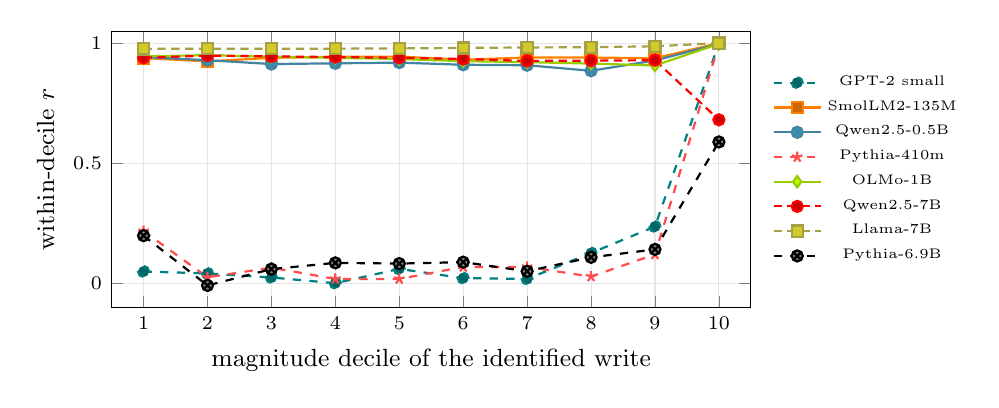
\begin{tikzpicture}\begin{axis}[width=0.8\linewidth, height=0.42\linewidth, xlabel={magnitude decile of the identified write}, ylabel={within-decile $r$}, xmin=0.5, xmax=10.5, ymin=-0.1, ymax=1.05, xtick={1,...,10}, grid=major, grid style={black!10}, legend style={font=\tiny, at={(1.02,0.5)}, anchor=west, draw=none}, tick label style={font=\scriptsize}, label style={font=\small}, cycle list name=exotic]
\addplot+[thick, dashed] coordinates {(1,0.05) (2,0.0421) (3,0.0251) (4,0.0014) (5,0.0608) (6,0.0226) (7,0.019) (8,0.127) (9,0.2371) (10,0.9998)};\addlegendentry{GPT-2 small}
\addplot+[thick] coordinates {(1,0.938) (2,0.924) (3,0.939) (4,0.943) (5,0.944) (6,0.931) (7,0.94) (8,0.94) (9,0.937) (10,1.0)};\addlegendentry{SmolLM2-135M}
\addplot+[thick] coordinates {(1,0.942) (2,0.929) (3,0.913) (4,0.916) (5,0.919) (6,0.91) (7,0.908) (8,0.885) (9,0.928) (10,0.997)};\addlegendentry{Qwen2.5-0.5B}
\addplot+[thick, dashed] coordinates {(1,0.218) (2,0.026) (3,0.066) (4,0.019) (5,0.019) (6,0.069) (7,0.069) (8,0.029) (9,0.121) (10,0.996)};\addlegendentry{Pythia-410m}
\addplot+[thick] coordinates {(1,0.945) (2,0.95) (3,0.943) (4,0.939) (5,0.934) (6,0.925) (7,0.921) (8,0.915) (9,0.907) (10,0.997)};\addlegendentry{OLMo-1B}
\addplot+[thick] coordinates {(1,0.939) (2,0.948) (3,0.945) (4,0.942) (5,0.939) (6,0.934) (7,0.926) (8,0.927) (9,0.929) (10,0.681)};\addlegendentry{Qwen2.5-7B}
\addplot+[thick] coordinates {(1,0.976) (2,0.977) (3,0.977) (4,0.977) (5,0.978) (6,0.98) (7,0.982) (8,0.983) (9,0.987) (10,1.0)};\addlegendentry{Llama-7B}
\addplot+[thick, dashed] coordinates {(1,0.199) (2,-0.008) (3,0.06) (4,0.086) (5,0.083) (6,0.089) (7,0.051) (8,0.109) (9,0.142) (10,0.589)};\addlegendentry{Pythia-6.9B}
\end{axis}\end{tikzpicture}\caption{Within-decile correlation per model. Solid lines are gated-MLP models, dashed lines non-gated.}\label{app:decilefig}\end{figure}
\begin{table}[H]\centering\footnotesize
\caption{The massive-channel test: FVU at $k=32$ over all coordinates and over all but the five highest-variance coordinates, for the weight dictionary and its rotation.}\label{app:channels}
\begin{adjustbox}{max width=\linewidth}
\begin{tabular}{lrrrrr}\toprule
Model & FVU@32, weight & off the top-5 coordinates & FVU@32, rotated & off the top-5 & variance in the top-5 coordinates \\ \midrule
SmolLM2-135M & 0.006 & 0.298 & 0.448 & 13.487 & 98.2\% \\
Qwen2.5-0.5B & 0.017 & 0.350 & 0.518 & 5.367 & 95.2\% \\
Pythia-410m & 0.050 & 0.539 & 0.594 & 3.035 & 91.2\% \\
OLMo-1B & 0.018 & 0.528 & 0.768 & 6.034 & 96.8\% \\
Qwen2.5-7B & 0.010 & 0.226 & 0.851 & 3.728 & 95.8\% \\
Llama-7B & 0.088 & 0.636 & 0.868 & 1.593 & 86.7\% \\
Pythia-6.9B & 0.309 & 0.678 & 0.869 & 1.005 & 55.5\% \\
\bottomrule\end{tabular}\end{adjustbox}
\end{table}
\begin{table}[H]\centering\footnotesize
\caption{Concentration of the largest true write. In all eight models the most frequent top-1 neuron takes a few percent of tokens, so top-1 recall measures identification across thousands of atoms.}\label{app:conc}
\begin{adjustbox}{max width=\linewidth}
\begin{tabular}{lrrrrrr}\toprule
Model & tokens & distinct top-1 neurons & most frequent & which & top five together & entropy, bits \\ \midrule
GPT-2 small & 8,192 & 916 & 4.7\% & mlp0\#132 & 16.5\% & 7.8 \\
SmolLM2-135M & 8,192 & 1,654 & 2.5\% & mlp0\#900 & 10.8\% & 8.9 \\
Qwen2.5-0.5B & 8,192 & 2,275 & 3.4\% & mlp0\#2290 & 9.4\% & 9.7 \\
Pythia-410m & 8,192 & 1,416 & 3.9\% & mlp0\#751 & 11.7\% & 8.9 \\
OLMo-1B & 8,192 & 2,763 & 2.4\% & mlp0\#1913 & 8.9\% & 10.1 \\
Qwen2.5-7B & 8,192 & 3,282 & 3.4\% & mlp9\#11283 & 10.5\% & 10.3 \\
Llama-7B & 8,192 & 2,831 & 4.0\% & mlp16\#4294 & 9.9\% & 10.2 \\
Pythia-6.9B & 8,192 & 1,677 & 8.4\% & mlp14\#2130 & 22.6\% & 8.5 \\
\bottomrule\end{tabular}\end{adjustbox}
\end{table}
\begin{table}[H]\centering\small
\caption{The GPT-2 evaluation on a Pile-derived sample. Reconstruction and attribution replicate; the block-3 role profile does not, which is why the paper treats roles as a property of a model on a distribution. Shuffled-null counter fraction on Pile: 0.668.}\label{app:pile}
\begin{adjustbox}{max width=\linewidth}
\begin{tabular}{lrr}\toprule
GPT-2 small & Pile sample (16,384 tokens) & WikiText-2 \\ \midrule
FVU@32, weight dictionary & 0.080 & 0.069 \\
FVU@32, rotated & 0.518 & 0.520 \\
top-1 recall, OMP & 0.562 & 0.647 \\
top-1 recall, one-shot & 0.660 & 0.766 \\
$r$ identified & 0.998 & 0.998 \\
$r$ unconditional & 0.647 & 0.648 \\
block 3 counter-aligned fraction & 0.379 & 0.525 \\
block 3 median birth survival & 0.77 & -0.09 \\
block 3 anchored fraction & 0.391 & 0.244 \\
\bottomrule\end{tabular}\end{adjustbox}
\end{table}
\begin{figure}[H]\centering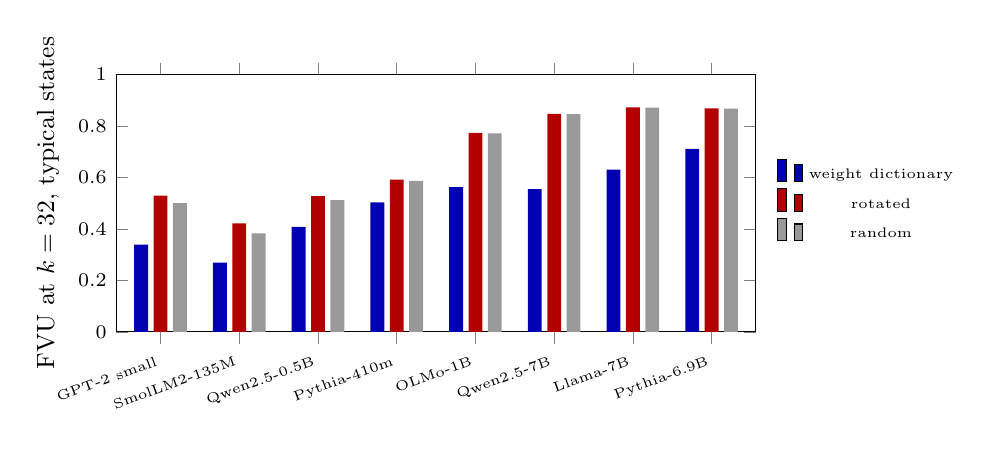
\begin{tikzpicture}\begin{axis}[width=0.8\linewidth, height=0.4\linewidth, ybar, bar width=5pt, ymin=0, ymax=1, ylabel={FVU at $k=32$, typical states}, symbolic x coords={GPT-2 small,SmolLM2-135M,Qwen2.5-0.5B,Pythia-410m,OLMo-1B,Qwen2.5-7B,Llama-7B,Pythia-6.9B}, xtick=data, x tick label style={font=\tiny, rotate=20, anchor=north east}, legend style={font=\tiny, at={(1.02,0.5)}, anchor=west, draw=none}, tick label style={font=\scriptsize}, label style={font=\small}, enlarge x limits=0.08]
\addplot[fill=blue!70!black, draw=none] coordinates {(GPT-2 small,0.3385) (SmolLM2-135M,0.2694) (Qwen2.5-0.5B,0.4076) (Pythia-410m,0.5031) (OLMo-1B,0.5628) (Qwen2.5-7B,0.5548) (Llama-7B,0.6306) (Pythia-6.9B,0.7110)};\addlegendentry{weight dictionary}
\addplot[fill=red!70!black, draw=none] coordinates {(GPT-2 small,0.5294) (SmolLM2-135M,0.4214) (Qwen2.5-0.5B,0.5272) (Pythia-410m,0.5918) (OLMo-1B,0.7731) (Qwen2.5-7B,0.8472) (Llama-7B,0.8723) (Pythia-6.9B,0.8680)};\addlegendentry{rotated}
\addplot[fill=black!40, draw=none] coordinates {(GPT-2 small,0.5002) (SmolLM2-135M,0.3828) (Qwen2.5-0.5B,0.5122) (Pythia-410m,0.5864) (OLMo-1B,0.7709) (Qwen2.5-7B,0.8458) (Llama-7B,0.8717) (Pythia-6.9B,0.8672)};\addlegendentry{random}
\end{axis}\end{tikzpicture}\caption{FVU at $k=32$ per model over the typical states on WikiText-2, from the sweep of Appendix~\ref{app:ci}, for the weight dictionary, its Gram-preserving rotation, and random directions. The rotation sits at the random floor in all eight models.}\label{app:fvufig}\end{figure}
\section{Write roles and null controls}\label{app:roles}
Table~\ref{app:nulls} gives, per block, the real role fractions next to the two nulls, and Table~\ref{app:quint} the counter-aligned fraction by magnitude quintile.
\begin{table}[H]\centering\scriptsize
\caption{Role fractions of each block's dominant writes on WikiText, against random replacement directions and shuffled write-state pairings. Each block's real counter fraction lies below its shuffled null; anchoring and reinforcing mass do not.}\label{app:nulls}
\begin{adjustbox}{max width=\linewidth}
\begin{tabular}{lrrrrrrrrrrr}\toprule
block & writes & median $s_{\mathrm{birth}}$ & counter, real & random dir. & shuffled & anchored, real & random dir. & shuffled & reinforcing, real & random dir. & shuffled \\ \midrule
0 & 39,193 & 1.29 & 0.019 & 0.498 & 0.512 & 0.679 & 0.003 & 0.061 & 0.291 & 0.000 & 0.058 \\
1 & 11,033 & 1.64 & 0.030 & 0.504 & 0.568 & 0.334 & 0.008 & 0.043 & 0.611 & 0.000 & 0.009 \\
2 & 9,989 & 1.02 & 0.197 & 0.495 & 0.637 & 0.403 & 0.012 & 0.064 & 0.335 & 0.000 & 0.021 \\
3 & 10,250 & -0.09 & 0.525 & 0.504 & 0.721 & 0.244 & 0.016 & 0.057 & 0.149 & 0.000 & 0.006 \\
4 & 2,661 & 1.47 & 0.037 & 0.493 & 0.594 & 0.482 & 0.023 & 0.044 & 0.458 & 0.000 & 0.011 \\
5 & 9,556 & 1.54 & 0.237 & 0.508 & 0.633 & 0.201 & 0.040 & 0.067 & 0.524 & 0.000 & 0.014 \\
6 & 15,622 & 1.94 & 0.054 & 0.501 & 0.580 & 0.172 & 0.048 & 0.061 & 0.754 & 0.000 & 0.014 \\
\bottomrule\end{tabular}\end{adjustbox}
\end{table}
\begin{table}[H]\centering\small
\caption{Counter-aligned fraction by magnitude quintile of the write. Block 3 leads in each quintile.}\label{app:quint}
\begin{adjustbox}{max width=\linewidth}
\begin{tabular}{lrrrrr}\toprule
block & quintile 1, smallest & 2 & 3 & 4 & 5, largest \\ \midrule
0 & 0.069 & 0.030 & 0.011 & 0.007 & 0.002 \\
1 & 0.034 & 0.031 & 0.039 & 0.022 & 0.025 \\
2 & 0.270 & 0.213 & 0.203 & 0.170 & 0.097 \\
3 & 0.545 & 0.574 & 0.563 & 0.505 & 0.230 \\
4 & 0.087 & 0.032 & 0.019 & 0.016 & 0.009 \\
5 & 0.378 & 0.315 & 0.177 & 0.044 & 0.012 \\
6 & 0.102 & 0.068 & 0.046 & 0.028 & 0.022 \\
\bottomrule\end{tabular}\end{adjustbox}
\end{table}
\section{The channel-447 circuit}\label{app:circuit}
Tables~\ref{app:dose} to~\ref{app:leash} and Figure~\ref{app:traj} are the intervention results of Section~\ref{sec:circuit} in full.
\begin{table}[H]\centering\footnotesize
\caption{Relative activation change of each active block-3 neuron when channel 447 is scaled at the block 2/3 boundary; 1,236 neurons respond inversely to both scalings by 10\% or more.}\label{app:dose}
\begin{adjustbox}{max width=\linewidth}
\begin{tabular}{lrrrrrrrrr}\toprule
Scaling channel 447 & active neurons & p5 & p25 & median & p75 & p95 & moved 10\% or more & neuron 614 & its percentile \\ \midrule
channel halved & 2948 & +0.2\% & +6.4\% & +9.0\% & +14.0\% & +44.6\% & 45\% & +27.5\% & 90 \\
channel times 1.5 & 2948 & -51.9\% & -17.8\% & -12.0\% & -9.1\% & -5.4\% & 68\% & -21.9\% & 82 \\
\bottomrule\end{tabular}\end{adjustbox}
\end{table}
\begin{table}[H]\centering\footnotesize
\caption{The frozen-normalization control: with block 3's LayerNorm statistics held at their clean-run values, the block-wide response collapses while neuron 614 keeps most of its own.}\label{app:frozen}
\begin{adjustbox}{max width=\linewidth}
\begin{tabular}{lrrrrrrr}\toprule
Block 3 pre-MLP LayerNorm & median, halved & median, times 1.5 & p95, halved & inverse responders & neuron 614, halved & times 1.5 & percentile \\ \midrule
LayerNorm free & +9.0\% & -12.0\% & +44.6\% & 1,236 & +27.5\% & -21.9\% & 90 \\
LayerNorm frozen at clean statistics & -0.5\% & -2.1\% & +17.4\% & 233 & +15.5\% & -12.3\% & 94 \\
\bottomrule\end{tabular}\end{adjustbox}
\end{table}
\begin{table}[H]\centering\small
\caption{Behavioral cost of ablating the strongest channel-447 counter-writers of block 3 (clean cross-entropy 3.6291). The top nine are neurons 614, 2664, 2885, 1995, 2723, 548, 1080, 2600, 2607.}\label{app:ablate}
\begin{adjustbox}{max width=\linewidth}
\begin{tabular}{lrr}\toprule
ablated block-3 counter-writers, top $k$ by counter energy & ablated write energy & $\Delta$CE \\ \midrule
1 & 417,084 & +0.0043 \\
3 & 553,816 & +0.0235 \\
5 & 590,306 & +0.0248 \\
7 & 619,043 & +0.0243 \\
9 & 640,105 & +0.0242 \\
random 9, set 1 & 7,986 & -0.0002 \\
random 9, set 2 & 12,113 & +0.0011 \\
random 9, set 3 & 8,693 & +0.0008 \\
\bottomrule\end{tabular}\end{adjustbox}
\end{table}
\begin{figure}[H]\centering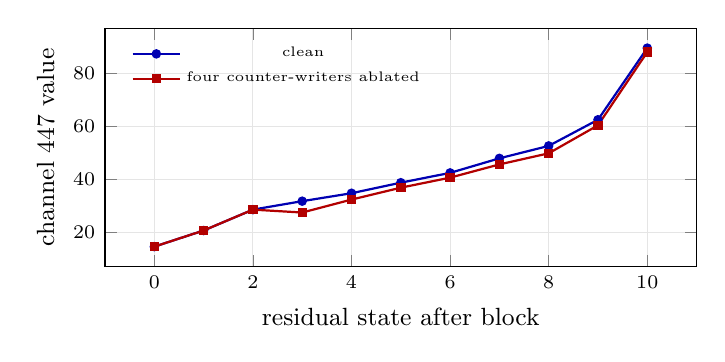
\begin{tikzpicture}\begin{axis}[width=0.75\linewidth, height=0.38\linewidth, xlabel={residual state after block}, ylabel={channel 447 value}, xtick={0,2,...,10}, grid=major, grid style={black!10}, legend style={font=\tiny, at={(0.03,0.97)}, anchor=north west, draw=none, fill=none}, tick label style={font=\scriptsize}, label style={font=\small}]
\addplot[thick, blue!70!black, mark=*, mark size=1.3pt] coordinates {(0,14.6) (1,20.7) (2,28.6) (3,31.8) (4,34.8) (5,38.8) (6,42.5) (7,48.0) (8,52.7) (9,62.6) (10,89.7)};\addlegendentry{clean}
\addplot[thick, red!70!black, mark=square*, mark size=1.3pt] coordinates {(0,14.6) (1,20.7) (2,28.6) (3,27.5) (4,32.4) (5,36.9) (6,40.7) (7,45.7) (8,49.9) (9,60.5) (10,88.2)};\addlegendentry{four counter-writers ablated}
\end{axis}\end{tikzpicture}\caption{Restoration: channel 447 in the raw residual state after each block, with and without the four strongest counter-writers. The ablation opens a gap after block 3 that later components close by the state after block 10, the input of block 11, which is the readout of the text; the state after block 11 is only available through the final normalization and is omitted.}\label{app:traj}\end{figure}
\begin{table}[H]\centering\small
\caption{Per-component contribution to the restoration, summing to -2.22. The largest single restorers are mlp7\#2402 (+1.09), mlp9\#840 (+0.73), mlp10\#900 (+0.64), mlp5\#1888 (+0.53), mlp6\#834 (+0.49).}\label{app:compensate}
\begin{adjustbox}{max width=\linewidth}
\begin{tabular}{lr}\toprule
Component & change in channel 447 write, ablated minus clean \\ \midrule
mlp3 & -4.313 \\
attn4 & +0.340 \\
mlp4 & +1.661 \\
attn5 & +0.755 \\
mlp5 & -0.406 \\
attn6 & +0.226 \\
mlp6 & -0.055 \\
attn7 & -1.863 \\
mlp7 & +1.400 \\
attn8 & -0.535 \\
mlp8 & +0.023 \\
attn9 & -0.570 \\
mlp9 & +1.212 \\
attn10 & -1.415 \\
mlp10 & +2.047 \\
attn11 & +3.127 \\
mlp11 & -3.855 \\
\bottomrule\end{tabular}\end{adjustbox}
\end{table}
\begin{table}[H]\centering\footnotesize
\caption{The reserve bank: channel-insensitive later neurons whose channel-447 writes rise when the four counter-writers are ablated, with random controls for comparison. The primary, neuron 614, is one of the ablated four; its intact write is shown for scale and is zero under the ablation.}\label{app:reserves}
\begin{adjustbox}{max width=\linewidth}
\begin{tabular}{lrrrrrr}\toprule
Neuron & role & gain, halved & gain, times 1.5 & channel-447 write, intact & under group ablation & change \\ \midrule
mlp5\#1888 & reserve & -0.032 & +0.049 & 2.00 & 2.53 & +26\% \\
mlp6\#834 & reserve & -0.030 & +0.031 & 1.84 & 2.33 & +26\% \\
mlp7\#2402 & reserve & -0.031 & +0.063 & 2.13 & 3.23 & +51\% \\
mlp9\#840 & reserve & -0.008 & +0.007 & 7.20 & 7.93 & +10\% \\
mlp10\#900 & reserve & -0.011 & +0.023 & 6.20 & 6.84 & +10\% \\
mlp3\#614 & primary & +0.275 & -0.221 & 4.31 & ablated &  \\
mlp5\#1159 & control & +0.004 & -0.005 & 0.01 & 0.01 & -10\% \\
mlp6\#902 & control & -0.005 & +0.009 & 0.04 & 0.04 & -2\% \\
mlp7\#327 & control & +0.002 & -0.010 & -0.09 & -0.08 & -2\% \\
mlp9\#2312 & control & +0.001 & -0.004 & 0.00 & 0.00 & +0\% \\
mlp10\#2632 & control & +0.012 & -0.014 & -0.03 & -0.03 & +0\% \\
\bottomrule\end{tabular}\end{adjustbox}
\end{table}
\begin{table}[H]\centering\small
\caption{Locating the suppression: which part of the counter-writers' output holds the reserve bank back (clean channel 447 at layer 11: 89.7).}\label{app:leash}
\begin{adjustbox}{max width=\linewidth}
\begin{tabular}{lrrr}\toprule
Write-editing condition & channel 447 at layer 11 & mean reserve response & mean control response \\ \midrule
ablate the four counter-writers & 88.2 & +0.248 & -0.010 \\
remove only the non-channel components of their writes & 91.5 & +0.186 & -0.016 \\
remove only the channel-447 component & 87.0 & +0.046 & +0.007 \\
remove neuron 614's non-channel component alone & 89.6 & -0.002 & +0.000 \\
\bottomrule\end{tabular}\end{adjustbox}
\end{table}
\section{Nomination comparisons}\label{app:bakeoff}
\paragraph{Pre-registered battery.} Fixed in code before any result existed, and identical for each arm. Universe: GPT-2 small MLP neurons in blocks 2 to 8, excluding each neuron studied in the circuit work and any neuron with more than 0.15 of its direction energy in the known massive channels 138, 266, 447, 481 and 496. For a nominee $j$: (1) firing tokens are those with $|c_j|$ in the neuron\textquotesingle s own top 5\%, at least 200; (2) the ledger names the top upstream MLP contributor $u$ along $\mathbf{d}_j$ on those tokens; (3) $u$ is ablated, and as a matched control a random neuron from $u$\textquotesingle s block, measuring on the firing tokens the change in $\langle \mathbf{h}, \mathbf{d}_j\rangle$ after block $j$ against the prediction from $u$\textquotesingle s direct contribution, and the relative change in $|a_j|$; (4) Tier 1 holds when the sign matches the prediction, the magnitude lies within 0.2 to 2 times the prediction, and exceeds 3 times the control; Tier 2 holds when the relative response is at least 0.02 and at least 3 times the control. Arms: WDD ranks by unconditional counter-alignment write energy; the outlier arm by activation excess kurtosis times mean write magnitude; the correlation arm, added at ten per arm, by maximum absolute activation correlation with any upstream MLP neuron.
\begin{table}[H]\centering\footnotesize
\caption{The pilot at three nominees per arm. Fisher exact, one-sided: Tier 2, $p=0.05$; passing either tier, $p=0.20$.}\label{app:pilot}
\begin{adjustbox}{max width=\linewidth}
\begin{tabular}{lrrrrrrrr}\toprule
Nominee & partner $u$ & predicted & measured & control & response & control & Tier 1 & Tier 2 \\ \midrule
\multicolumn{9}{l}{\emph{WDD arm}} \\
mlp6\#437 & mlp5\#1790 & -2.91 & +0.81 & -0.01 & +0.238 & -0.000 & no & yes \\
mlp8\#583 & mlp2\#676 & +3.74 & +9.86 & -0.01 & -0.924 & +0.001 & no & yes \\
mlp2\#1195 & mlp0\#1121 & +1.08 & +0.20 & +0.01 & -0.200 & -0.001 & no & yes \\
\multicolumn{9}{l}{\emph{outlier arm}} \\
mlp8\#1807 & mlp2\#666 & +2.87 & +0.43 & -0.00 & +0.002 & -0.000 & no & no \\
mlp6\#861 & mlp3\#614 & +0.17 & -0.01 & -0.01 & -0.005 & -0.001 & no & no \\
mlp8\#2535 & mlp7\#2367 & -0.32 & -0.23 & +0.00 & +0.017 & +0.001 & yes & no \\
\bottomrule\end{tabular}\end{adjustbox}
\end{table}
\begin{table}[H]\centering\small
\caption{Tallies at ten and thirty nominees per arm. One-sided Fisher exact tests at thirty per arm: WDD against the outlier screen, Tier 2 $p=0.004$ and Tier 1 $p=0.15$; the correlation screen against WDD, Tier 2 $p=0.37$ and Tier 1 $p=0.0017$. The first ten nominees of each thirty-nominee arm are the ten-nominee arms, and their tallies reproduce exactly.}\label{app:tallies}
\begin{adjustbox}{max width=\linewidth}
\begin{tabular}{lrrrr}\toprule
Arm & Tier 1 & Tier 2 & either & both \\ \midrule
\multicolumn{5}{l}{\emph{ten nominees per arm}} \\
WDD & 4/10 & 8/10 & 8/10 & 4/10 \\
outlier & 2/10 & 6/10 & 7/10 & 1/10 \\
corr & 9/10 & 8/10 & 10/10 & 7/10 \\
\multicolumn{5}{l}{\emph{thirty nominees per arm}} \\
WDD & 16/30 & 23/30 & 27/30 & 12/30 \\
outlier & 11/30 & 12/30 & 22/30 & 1/30 \\
corr & 27/30 & 25/30 & 30/30 & 22/30 \\
\bottomrule\end{tabular}\end{adjustbox}
\end{table}
\begin{figure}[H]\centering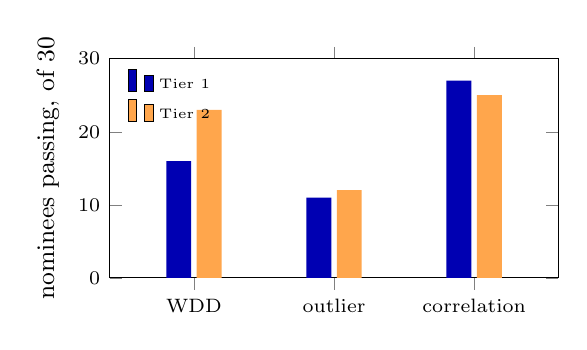
\begin{tikzpicture}\begin{axis}[width=0.6\linewidth, height=0.36\linewidth, ybar, bar width=9pt, ymin=0, ymax=30, ylabel={nominees passing, of 30}, symbolic x coords={WDD,outlier,correlation}, xtick=data, legend style={font=\tiny, at={(0.02,0.98)}, anchor=north west, draw=none, fill=none}, tick label style={font=\scriptsize}, label style={font=\small}, enlarge x limits=0.3]
\addplot[fill=blue!70!black, draw=none] coordinates {(WDD,16) (outlier,11) (correlation,27)};\addlegendentry{Tier 1}
\addplot[fill=orange!70, draw=none] coordinates {(WDD,23) (outlier,12) (correlation,25)};\addlegendentry{Tier 2}
\end{axis}\end{tikzpicture}\caption{The thirty-per-arm bake-off.}\label{app:bakefig}\end{figure}
\begin{center}\scriptsize
\begin{longtable}{llrrrrrcc}
\caption{Each nominee of the thirty-per-arm run, with the arm or arms that nominated it and its battery. Columns as in Table~\ref{app:pilot}.}\label{app:n30}\\ \toprule
Nominee & arms & partner & predicted & measured & control & response & control & T1/T2 \\ \midrule \endfirsthead
\toprule Nominee & arms & partner & predicted & measured & control & response & control & T1/T2 \\ \midrule \endhead
\bottomrule \endfoot
mlp2\#34 & correlation & mlp0\#1561 & -1.87 & -2.17 & -0.03 & -0.282 & -0.002 & yes/yes \\
mlp2\#352 & correlation & mlp1\#3020 & -1.52 & -2.12 & +0.00 & -0.780 & +0.000 & yes/yes \\
mlp2\#589 & WDD & mlp0\#1430 & +0.23 & -0.00 & +0.00 & -0.003 & -0.000 & no/no \\
mlp2\#1173 & outlier, correlation & mlp0\#944 & +0.75 & +0.41 & -0.00 & -0.001 & -0.000 & yes/no \\
mlp2\#1279 & correlation & mlp0\#2009 & +0.78 & -0.24 & -0.01 & +0.062 & +0.001 & no/yes \\
mlp2\#2769 & WDD, correlation & mlp0\#1175 & +5.99 & +8.33 & +0.01 & -0.977 & +0.001 & yes/yes \\
mlp2\#2830 & correlation & mlp0\#1175 & -6.34 & -9.71 & +0.00 & -0.946 & +0.000 & yes/yes \\
mlp2\#2898 & correlation & mlp0\#371 & -0.45 & -0.53 & -0.00 & -0.000 & -0.000 & yes/no \\
mlp3\#176 & WDD & mlp1\#79 & +0.93 & +0.57 & -0.00 & -0.223 & -0.003 & yes/yes \\
mlp3\#489 & outlier & mlp2\#2714 & -0.65 & +0.30 & +0.01 & +0.033 & +0.001 & no/yes \\
mlp4\#825 & correlation & mlp2\#666 & +8.87 & +3.08 & +0.00 & +0.073 & +0.001 & yes/yes \\
mlp4\#1322 & WDD & mlp3\#614 & -1.36 & -0.08 & -0.01 & +0.069 & -0.001 & no/yes \\
mlp4\#2266 & correlation & mlp0\#1451 & -1.09 & -1.58 & +0.01 & -0.367 & -0.002 & yes/yes \\
mlp4\#2555 & correlation & mlp2\#666 & +6.77 & +2.26 & +0.00 & +0.005 & +0.001 & yes/no \\
mlp4\#2806 & correlation & mlp0\#2054 & -4.25 & -7.03 & -0.03 & -0.457 & -0.002 & yes/yes \\
mlp5\#464 & correlation & mlp4\#2622 & -2.05 & -4.26 & -0.01 & -0.531 & -0.002 & no/yes \\
mlp5\#1504 & correlation & mlp0\#132 & -7.66 & -7.42 & -0.00 & -0.251 & +0.001 & yes/yes \\
mlp5\#1526 & outlier & mlp3\#2664 & -0.21 & +0.13 & +0.01 & -0.026 & +0.001 & no/yes \\
mlp5\#2073 & correlation & mlp3\#2614 & -4.31 & -1.06 & -0.00 & -0.258 & -0.000 & yes/yes \\
mlp5\#2078 & outlier & mlp3\#614 & -0.72 & +0.03 & -0.00 & -0.028 & +0.001 & no/yes \\
mlp5\#2084 & correlation & mlp2\#666 & -7.49 & -1.81 & -0.00 & -0.008 & +0.003 & yes/no \\
mlp5\#2256 & outlier, correlation & mlp2\#666 & +10.51 & +2.75 & -0.00 & +0.034 & -0.000 & yes/yes \\
mlp6\#203 & correlation & mlp2\#2830 & -6.54 & -11.85 & -0.01 & -0.920 & -0.003 & yes/yes \\
mlp6\#522 & WDD & mlp4\#1727 & -0.71 & -0.31 & +0.00 & +0.070 & +0.001 & yes/yes \\
mlp6\#1393 & correlation & mlp0\#874 & -2.06 & -1.65 & -0.01 & -0.167 & -0.000 & yes/yes \\
mlp6\#1681 & outlier & mlp2\#2714 & +0.16 & -0.01 & -0.00 & -0.005 & +0.000 & no/no \\
mlp6\#1912 & correlation & mlp0\#908 & -3.59 & -1.33 & -0.02 & -0.053 & -0.001 & yes/yes \\
mlp6\#1985 & WDD & mlp5\#1856 & -0.57 & +0.25 & -0.00 & +0.323 & +0.000 & no/yes \\
mlp6\#2006 & outlier & mlp3\#614 & +0.32 & +0.02 & +0.00 & -0.015 & +0.000 & no/no \\
mlp6\#2081 & correlation & mlp2\#666 & -3.21 & -0.77 & -0.00 & +0.001 & -0.001 & yes/no \\
mlp6\#2374 & correlation & mlp0\#1218 & -1.83 & -1.63 & +0.01 & -0.064 & +0.000 & yes/yes \\
mlp6\#2667 & correlation & mlp0\#753 & -1.21 & -1.96 & +0.00 & -0.315 & -0.000 & yes/yes \\
mlp6\#2674 & WDD & mlp2\#2830 & +5.93 & +10.26 & -0.00 & -0.920 & +0.003 & yes/yes \\
mlp6\#2703 & correlation & mlp0\#132 & -7.57 & -7.46 & +0.01 & -0.249 & -0.000 & yes/yes \\
mlp6\#2984 & outlier & mlp5\#1888 & -0.19 & -0.09 & +0.00 & +0.005 & +0.000 & yes/no \\
mlp6\#3048 & WDD & mlp5\#1790 & -2.05 & +0.24 & +0.00 & +0.222 & +0.000 & no/yes \\
mlp7\#6 & outlier & mlp5\#1790 & +0.51 & +0.15 & -0.01 & -0.013 & -0.000 & yes/no \\
mlp7\#549 & correlation & mlp0\#132 & -6.32 & -5.84 & -0.00 & -0.173 & -0.000 & yes/yes \\
mlp7\#658 & correlation & mlp0\#2963 & -1.29 & -2.42 & -0.01 & -0.294 & -0.001 & yes/yes \\
mlp7\#889 & outlier & mlp3\#614 & +0.59 & +0.13 & -0.01 & +0.013 & -0.001 & yes/no \\
mlp7\#991 & WDD & mlp1\#1825 & -0.37 & -0.22 & -0.00 & -0.427 & -0.003 & yes/yes \\
mlp7\#1600 & WDD & mlp5\#1790 & -0.42 & -0.13 & -0.00 & +0.005 & +0.001 & yes/no \\
mlp7\#1729 & WDD & mlp6\#3039 & +0.60 & -0.04 & +0.00 & +0.033 & +0.000 & no/yes \\
mlp7\#2083 & WDD & mlp6\#2799 & -0.70 & -0.91 & +0.00 & +0.292 & +0.001 & yes/yes \\
mlp7\#2202 & correlation & mlp6\#2081 & -0.75 & -1.48 & -0.00 & -0.348 & -0.000 & yes/yes \\
mlp7\#2214 & outlier & mlp3\#614 & -0.38 & -0.05 & -0.00 & -0.011 & +0.001 & no/no \\
mlp7\#2348 & outlier & mlp5\#1790 & -0.26 & +0.10 & +0.01 & -0.035 & +0.001 & no/yes \\
mlp7\#2398 & WDD & mlp3\#1545 & -1.12 & -0.25 & -0.00 & -0.008 & +0.000 & yes/no \\
mlp7\#2489 & WDD & mlp5\#1790 & -2.05 & +0.40 & -0.00 & -0.072 & +0.001 & no/yes \\
mlp7\#2517 & WDD & mlp6\#1879 & +0.66 & +0.40 & +0.00 & -0.269 & +0.004 & yes/yes \\
mlp7\#2531 & WDD & mlp2\#2771 & +1.57 & -0.05 & -0.00 & -0.030 & +0.001 & no/yes \\
mlp7\#2750 & outlier & mlp6\#3039 & +0.38 & +0.01 & +0.00 & +0.015 & +0.000 & no/no \\
mlp8\#13 & WDD & mlp7\#2367 & -1.43 & +1.34 & +0.00 & +0.013 & -0.000 & no/no \\
mlp8\#15 & WDD & mlp0\#132 & +1.09 & +0.92 & -0.00 & -0.058 & -0.000 & yes/yes \\
mlp8\#82 & outlier & mlp5\#1790 & +0.53 & +0.29 & +0.00 & +0.004 & +0.000 & yes/no \\
mlp8\#201 & correlation & mlp7\#1588 & -0.55 & -0.73 & -0.01 & -0.143 & -0.001 & yes/yes \\
mlp8\#428 & WDD & mlp7\#2367 & +0.61 & -0.73 & +0.03 & -0.100 & +0.003 & no/yes \\
mlp8\#529 & WDD & mlp7\#2690 & -0.79 & -0.45 & -0.01 & +0.219 & -0.004 & yes/yes \\
mlp8\#599 & WDD & mlp7\#2367 & +0.44 & -0.67 & +0.00 & +0.010 & -0.001 & no/no \\
mlp8\#687 & outlier & mlp7\#2367 & +0.88 & -0.66 & -0.00 & +0.120 & -0.001 & no/yes \\
mlp8\#825 & WDD & mlp7\#1012 & +0.90 & -0.24 & -0.00 & -0.288 & -0.003 & no/yes \\
mlp8\#1108 & outlier & mlp7\#2402 & +0.22 & +0.12 & +0.01 & -0.001 & +0.002 & yes/no \\
mlp8\#1182 & outlier & mlp7\#2367 & +0.30 & +0.61 & +0.01 & +0.010 & +0.002 & no/no \\
mlp8\#1203 & WDD & mlp7\#2402 & +0.44 & +0.28 & -0.02 & +0.011 & +0.001 & yes/no \\
mlp8\#1276 & WDD & mlp7\#2402 & +0.35 & +0.05 & +0.01 & -0.027 & +0.001 & no/yes \\
mlp8\#1332 & WDD & mlp7\#79 & +1.30 & +0.57 & +0.01 & -0.283 & +0.000 & yes/yes \\
mlp8\#1333 & correlation & mlp7\#658 & -1.47 & -1.74 & -0.01 & -0.181 & -0.003 & yes/yes \\
mlp8\#1423 & outlier & mlp7\#2402 & +0.62 & +0.34 & -0.00 & -0.007 & -0.000 & yes/no \\
mlp8\#1542 & WDD & mlp7\#2589 & +0.83 & -0.04 & +0.01 & -0.163 & -0.002 & no/yes \\
mlp8\#1749 & outlier & mlp7\#2367 & -0.28 & +0.53 & -0.01 & +0.078 & -0.002 & no/yes \\
mlp8\#1764 & WDD & mlp7\#2086 & -0.20 & -0.12 & +0.00 & +0.040 & +0.002 & yes/yes \\
mlp8\#1827 & WDD & mlp7\#2402 & -1.35 & -0.64 & +0.00 & +0.065 & +0.001 & yes/yes \\
mlp8\#1864 & WDD & mlp5\#1790 & -0.33 & -0.10 & -0.00 & +0.000 & -0.002 & yes/no \\
mlp8\#1981 & WDD & mlp5\#1790 & -0.45 & +0.20 & +0.04 & -0.030 & +0.005 & no/yes \\
mlp8\#2036 & outlier & mlp7\#2367 & -1.11 & +1.86 & +0.04 & -0.010 & +0.001 & no/no \\
mlp8\#2087 & outlier & mlp7\#2367 & +0.78 & -1.10 & -0.02 & +0.010 & -0.001 & no/no \\
mlp8\#2162 & outlier & mlp7\#2367 & +0.56 & -0.77 & -0.01 & +0.061 & -0.002 & no/yes \\
mlp8\#2346 & outlier & mlp7\#2367 & +1.36 & -1.62 & +0.00 & +0.015 & -0.000 & no/no \\
mlp8\#2387 & outlier & mlp5\#1790 & -0.23 & -0.12 & +0.01 & -0.002 & +0.000 & yes/no \\
mlp8\#2402 & outlier & mlp7\#2402 & +0.21 & +0.10 & -0.00 & -0.010 & -0.000 & yes/no \\
mlp8\#2469 & outlier & mlp7\#2367 & +1.66 & -2.13 & -0.00 & +0.036 & -0.000 & no/yes \\
mlp8\#2532 & outlier & mlp4\#1894 & +0.18 & +0.08 & -0.00 & -0.007 & +0.000 & yes/no \\
mlp8\#2543 & outlier & mlp7\#2367 & +1.08 & -1.11 & +0.00 & +0.039 & +0.000 & no/yes \\
mlp8\#2687 & correlation & mlp6\#2081 & -1.35 & -3.27 & -0.01 & -0.482 & -0.001 & no/yes \\
mlp8\#2793 & outlier & mlp7\#2367 & +1.38 & -1.66 & +0.01 & +0.101 & +0.002 & no/yes \\
mlp8\#2836 & outlier & mlp7\#2367 & -0.29 & +1.08 & -0.01 & +0.280 & -0.006 & no/yes \\
mlp8\#2988 & correlation & mlp7\#2233 & -2.41 & -2.36 & +0.01 & -0.209 & +0.001 & yes/yes \\
\end{longtable}\end{center}
\section{Independent recomputation}\label{app:audit}
\begin{table}[H]\centering\small
\caption{An independent re-implementation of the dictionary, the attribution and the dose response, written from the description in the text with its own hooks, batching and seeds, on the same 32{,}768 tokens. The deterministic quantities agree to the printed precision and the dose response to within 0.2 percentage points; the rotation control draws a fresh random rotation (seed 777), so its value is near but not equal to that of Section~\ref{sec:recon}.}\label{app:audit-table}
\begin{adjustbox}{max width=\linewidth}
\begin{tabular}{lrr}\toprule
Quantity & paper & recomputed \\ \midrule
FVU at $k=32$, weight dictionary & 0.069 & 0.069 \\
FVU at $k=32$, rotated (fresh rotation, seed 777) & 0.549 & 0.517 \\
top-1 recall, OMP & 0.647 & 0.647 \\
$r$ identified & 0.998 & 0.998 \\
$r$ unconditional & 0.648 & 0.648 \\
neuron 614 response, channel halved & +27.5\% & +27.5\% \\
neuron 614 response, channel times 1.5 & -22.1\% & -21.9\% \\
\bottomrule\end{tabular}\end{adjustbox}
\end{table}
\section{Confidence intervals and the second corpus}\label{app:ci}
All numbers here come from \texttt{exp\_z2\_ci}, an implementation of the family sweep written from the description in Sections~\ref{sec:method} and~\ref{sec:setup} independently of the individual experiment scripts, run under one protocol for all eight models: 32{,}768 evaluation states per model and corpus, the same three dictionaries, OMP with $k=64$ read at 32 and 64, one-shot attribution, and a bootstrap over the 64 evaluation sequences with 1{,}000 resamples. Brackets are 95\% percentile intervals. GPT-2 keeps the conventions of Section~\ref{sec:setup} (a disjoint centering slice for reconstruction, the evaluation mean for attribution); the other families center on eight disjoint chunks throughout. Table~\ref{app:ci-old} sets its point estimates beside those of the individual experiment scripts.
\begin{table}[H]\centering\scriptsize
\caption{Reconstruction of the typical states on WikiText-2 with 95\% bootstrap intervals over sequences. Off top-5 removes the five highest-variance coordinates from numerator and denominator.}\label{app:ci-recon-wikitext}
\begin{adjustbox}{max width=\linewidth}
\begin{tabular}{lrrrrrrrr}\toprule
Model & FVU@32 weight & FVU@64 weight & FVU@32 rotated & FVU@64 rotated & FVU@32 random & off top-5, weight & off top-5, rotated & top-5 share \\ \midrule
GPT-2 small & 0.338 [0.337, 0.340] & 0.179 [0.179, 0.180] & 0.529 [0.529, 0.530] & 0.288 & 0.500 [0.500, 0.500] & 0.38 & 0.56 & 82.1\% \\
SmolLM2-135M & 0.269 [0.268, 0.270] & 0.113 [0.113, 0.114] & 0.421 [0.421, 0.422] & 0.179 & 0.383 [0.383, 0.383] & 0.34 & 0.49 & 98.2\% \\
Qwen2.5-0.5B & 0.408 [0.407, 0.408] & 0.219 [0.219, 0.219] & 0.527 [0.527, 0.527] & 0.282 & 0.512 [0.512, 0.512] & 0.44 & 0.55 & 95.4\% \\
Pythia-410m & 0.503 [0.502, 0.504] & 0.303 [0.302, 0.303] & 0.592 [0.592, 0.592] & 0.359 & 0.586 [0.586, 0.587] & 0.54 & 0.62 & 91.3\% \\
OLMo-1B & 0.563 [0.561, 0.564] & 0.435 [0.433, 0.436] & 0.773 [0.773, 0.773] & 0.611 & 0.771 [0.771, 0.771] & 0.60 & 0.79 & 96.7\% \\
Qwen2.5-7B & 0.555 [0.551, 0.558] & 0.459 [0.456, 0.462] & 0.847 [0.847, 0.847] & 0.729 & 0.846 [0.846, 0.846] & 0.68 & 0.88 & 95.8\% \\
Llama-7B & 0.631 [0.628, 0.633] & 0.533 [0.531, 0.535] & 0.872 [0.872, 0.872] & 0.772 & 0.872 [0.872, 0.872] & 0.66 & 0.88 & 86.9\% \\
Pythia-6.9B & 0.711 [0.709, 0.713] & 0.610 [0.609, 0.612] & 0.868 [0.868, 0.868] & 0.764 & 0.867 [0.867, 0.867] & 0.74 & 0.87 & 55.9\% \\
\bottomrule\end{tabular}\end{adjustbox}
\end{table}
\begin{table}[H]\centering\scriptsize
\caption{The sink states on WikiText-2: how many of the 32{,}768 states exceed ten times the median norm, the variance they carry, and their reconstruction. The all-state columns are what an FVU over all states reports.}\label{app:ci-sink-wikitext}
\begin{adjustbox}{max width=\linewidth}
\begin{tabular}{lrrrrrrrr}\toprule
Model & sink states & smallest sink norm over median & share of variance & sink FVU@32 weight & rotated & random & all-state FVU@32 weight & rotated \\ \midrule
GPT-2 small & 64 & 44$\times$ & 79.7\% & 0.0003 [0.0003, 0.0003] & 0.532 & 0.508 & 0.069 & 0.531 \\
SmolLM2-135M & 64 & 155$\times$ & 98.1\% & 0.0005 [0.0005, 0.0005] & 0.421 & 0.390 & 0.006 & 0.421 \\
Qwen2.5-0.5B & 65 & 85$\times$ & 96.2\% & 0.0013 [0.0013, 0.0013] & 0.517 & 0.514 & 0.017 & 0.518 \\
Pythia-410m & 127 & 47$\times$ & 90.8\% & 0.0037 [0.0037, 0.0037] & 0.591 & 0.582 & 0.050 & 0.591 \\
OLMo-1B & 68 & 43$\times$ & 96.8\% & 0.0006 [0.0006, 0.0006] & 0.779 & 0.773 & 0.019 & 0.779 \\
Qwen2.5-7B & 65 & 203$\times$ & 99.0\% & 0.0039 [0.0038, 0.0040] & 0.840 & 0.843 & 0.010 & 0.840 \\
Llama-7B & 131 & 27$\times$ & 86.0\% & 0.0002 [0.0002, 0.0002] & 0.870 & 0.870 & 0.089 & 0.870 \\
Pythia-6.9B & 66 & 21$\times$ & 58.7\% & 0.0270 [0.0269, 0.0272] & 0.873 & 0.866 & 0.310 & 0.871 \\
\bottomrule\end{tabular}\end{adjustbox}
\end{table}
\begin{table}[H]\centering\scriptsize
\caption{Attribution on WikiText-2 with 95\% bootstrap intervals over sequences. The all-state correlations are carried by the few identified writes at the sink states, whose magnitudes dominate the statistic; the typical-state columns exclude them, and Table~\ref{app:ci-calib-wikitext} is the accuracy statement.}\label{app:ci-attrib-wikitext}
\begin{adjustbox}{max width=\linewidth}
\begin{tabular}{lrrrrrrrr}\toprule
Model & gated & top-1 recall, OMP & top-1 recall, one-shot & $r$ identified, all states & typical states & $r$ unconditional, all & typical & identified writes \\ \midrule
GPT-2 small & no & 0.647 [0.637, 0.657] & 0.766 [0.754, 0.776] & 0.998 [0.998, 0.998] & 0.582 & 0.648 [0.648, 0.648] & 0.505 & 48,220 \\
SmolLM2-135M & yes & 0.670 [0.661, 0.680] & 0.682 [0.676, 0.688] & 1.000 [1.000, 1.000] & 0.835 & 0.928 [0.927, 0.928] & 0.494 & 48,543 \\
Qwen2.5-0.5B & yes & 0.459 [0.451, 0.467] & 0.614 [0.604, 0.623] & 0.994 [0.993, 0.994] & 0.819 & 0.551 [0.543, 0.559] & 0.534 & 34,285 \\
Pythia-410m & no & 0.481 [0.472, 0.490] & 0.593 [0.584, 0.601] & 0.980 [0.979, 0.981] & 0.322 & 0.452 [0.446, 0.455] & 0.275 & 35,864 \\
OLMo-1B & yes & 0.693 [0.687, 0.699] & 0.779 [0.775, 0.784] & 0.997 [0.997, 0.998] & 0.907 & 0.971 [0.969, 0.972] & 0.762 & 59,579 \\
Qwen2.5-7B & yes & 0.673 [0.663, 0.685] & 0.004 [0.004, 0.005] & 0.554 [0.506, 0.595] & 0.887 & 0.308 [0.271, 0.343] & 0.742 & 54,625 \\
Llama-7B & yes & 0.981 [0.979, 0.983] & 0.895 [0.881, 0.906] & 0.999 [0.999, 0.999] & 0.982 & 0.998 [0.998, 0.998] & 0.970 & 93,027 \\
Pythia-6.9B & no & 0.787 [0.779, 0.795] & 0.646 [0.639, 0.653] & 0.539 [0.528, 0.551] & 0.645 & 0.424 [0.409, 0.439] & 0.482 & 67,509 \\
\bottomrule\end{tabular}\end{adjustbox}
\end{table}
\begin{table}[H]\centering\scriptsize
\caption{Calibration of the recovered coefficients of identified dominant writes on WikiText-2, typical states. Ratio is recovered over true; a ratio above one is over-estimation.}\label{app:ci-calib-wikitext}
\begin{adjustbox}{max width=\linewidth}
\begin{tabular}{lrrrrrrrrrrr}\toprule
Model & identified writes & negative & sign recovered & median relative error & within 25\% & ratio, decile 1 & 5 & 10 & rel. error, decile 1 & 5 & 10 \\ \midrule
GPT-2 small & 48,156 & 0\% & 99.8\% & 0.44 [0.44, 0.45] & 29.4\% & 1.66 & 1.42 & 1.45 & 0.66 & 0.42 & 0.45 \\
SmolLM2-135M & 48,479 & 50\% & 100.0\% & 0.54 [0.53, 0.54] & 26.0\% & 1.97 & 1.55 & 0.73 & 0.97 & 0.55 & 0.32 \\
Qwen2.5-0.5B & 34,220 & 47\% & 100.0\% & 0.46 [0.45, 0.46] & 26.5\% & 1.58 & 1.34 & 0.43 & 0.58 & 0.45 & 0.57 \\
Pythia-410m & 35,801 & 0\% & 99.9\% & 0.41 [0.40, 0.42] & 34.2\% & 1.75 & 1.43 & 1.04 & 0.75 & 0.43 & 0.27 \\
OLMo-1B & 59,503 & 46\% & 99.7\% & 0.34 [0.34, 0.34] & 35.0\% & 1.06 & 0.76 & 0.51 & 0.25 & 0.32 & 0.49 \\
Qwen2.5-7B & 54,601 & 51\% & 100.0\% & 0.50 [0.50, 0.51] & 17.6\% & 0.97 & 0.52 & 0.29 & 0.25 & 0.48 & 0.71 \\
Llama-7B & 92,755 & 49\% & 100.0\% & 0.25 [0.25, 0.25] & 49.8\% & 1.39 & 1.24 & 1.17 & 0.39 & 0.26 & 0.17 \\
Pythia-6.9B & 67,475 & 0\% & 100.0\% & 1.03 [1.02, 1.04] & 4.4\% & 2.19 & 2.03 & 1.86 & 1.19 & 1.03 & 0.86 \\
\bottomrule\end{tabular}\end{adjustbox}
\end{table}
\begin{table}[H]\centering\scriptsize
\caption{Within-decile correlation of recovered and true coefficients on WikiText-2 (point estimates; intervals in Figure~\ref{app:ci-decilefig-wikitext}). In the gated models about half of the writes are negative, so this signed correlation within a magnitude decile mostly records sign recovery, and Table~\ref{app:ci-calib-wikitext} is the accuracy statement.}\label{app:ci-deciles-wikitext}
\begin{adjustbox}{max width=\linewidth}
\begin{tabular}{lrrrrrrrrrr}\toprule
Model & 1 & 2 & 3 & 4 & 5 & 6 & 7 & 8 & 9 & 10 \\ \midrule
GPT-2 small & 0.05 & 0.04 & 0.03 & 0.00 & 0.06 & 0.02 & 0.02 & 0.13 & 0.24 & 1.00 \\
SmolLM2-135M & 0.94 & 0.92 & 0.94 & 0.95 & 0.94 & 0.93 & 0.94 & 0.94 & 0.93 & 1.00 \\
Qwen2.5-0.5B & 0.94 & 0.93 & 0.91 & 0.91 & 0.91 & 0.92 & 0.90 & 0.88 & 0.94 & 1.00 \\
Pythia-410m & 0.21 & 0.03 & 0.08 & 0.02 & -0.05 & -0.02 & 0.03 & 0.07 & -0.07 & 1.00 \\
OLMo-1B & 0.93 & 0.95 & 0.94 & 0.94 & 0.93 & 0.93 & 0.92 & 0.91 & 0.91 & 1.00 \\
Qwen2.5-7B & 0.94 & 0.95 & 0.94 & 0.94 & 0.94 & 0.94 & 0.94 & 0.94 & 0.94 & 0.70 \\
Llama-7B & 0.97 & 0.98 & 0.98 & 0.98 & 0.98 & 0.98 & 0.98 & 0.98 & 0.99 & 1.00 \\
Pythia-6.9B & 0.22 & 0.02 & 0.04 & 0.04 & 0.05 & 0.07 & 0.04 & 0.08 & 0.12 & 0.66 \\
\bottomrule\end{tabular}\end{adjustbox}
\end{table}
\begin{figure}[H]\centering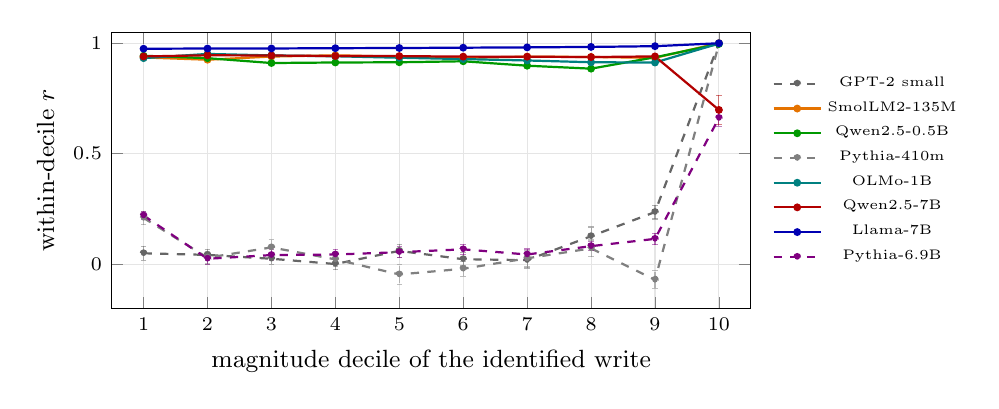
\begin{tikzpicture}\begin{axis}[width=0.8\linewidth, height=0.42\linewidth, xlabel={magnitude decile of the identified write}, ylabel={within-decile $r$}, xmin=0.5, xmax=10.5, ymin=-0.2, ymax=1.05, xtick={1,...,10}, grid=major, grid style={black!10}, legend style={font=\tiny, at={(1.02,0.5)}, anchor=west, draw=none}, tick label style={font=\scriptsize}, label style={font=\small}, error bars/y dir=both, error bars/y explicit]
\addplot[thick, dashed, color=black!60, mark=*, mark size=1pt, error bars/error bar style={opacity=0.5}] coordinates {(1,0.0499) +- (0,0.0322) (2,0.0425) +- (0,0.0256) (3,0.0251) +- (0,0.0254) (4,0.0013) +- (0,0.0260) (5,0.0607) +- (0,0.0294) (6,0.0230) +- (0,0.0301) (7,0.0189) +- (0,0.0354) (8,0.1270) +- (0,0.0416) (9,0.2362) +- (0,0.0312) (10,0.9998) +- (0,0.0000)};\addlegendentry{GPT-2 small}
\addplot[thick, color=orange!90!black, mark=*, mark size=1pt, error bars/error bar style={opacity=0.5}] coordinates {(1,0.9353) +- (0,0.0027) (2,0.9250) +- (0,0.0028) (3,0.9393) +- (0,0.0015) (4,0.9451) +- (0,0.0024) (5,0.9387) +- (0,0.0061) (6,0.9337) +- (0,0.0049) (7,0.9390) +- (0,0.0030) (8,0.9374) +- (0,0.0023) (9,0.9334) +- (0,0.0030) (10,0.9998) +- (0,0.0000)};\addlegendentry{SmolLM2-135M}
\addplot[thick, color=green!60!black, mark=*, mark size=1pt, error bars/error bar style={opacity=0.5}] coordinates {(1,0.9430) +- (0,0.0037) (2,0.9320) +- (0,0.0038) (3,0.9101) +- (0,0.0027) (4,0.9125) +- (0,0.0033) (5,0.9135) +- (0,0.0029) (6,0.9180) +- (0,0.0033) (7,0.8980) +- (0,0.0033) (8,0.8846) +- (0,0.0040) (9,0.9360) +- (0,0.0046) (10,0.9962) +- (0,0.0009)};\addlegendentry{Qwen2.5-0.5B}
\addplot[thick, dashed, color=gray, mark=*, mark size=1pt, error bars/error bar style={opacity=0.5}] coordinates {(1,0.2098) +- (0,0.0308) (2,0.0299) +- (0,0.0286) (3,0.0764) +- (0,0.0343) (4,0.0224) +- (0,0.0321) (5,-0.0458) +- (0,0.0435) (6,-0.0202) +- (0,0.0343) (7,0.0271) +- (0,0.0364) (8,0.0720) +- (0,0.0381) (9,-0.0702) +- (0,0.0402) (10,0.9959) +- (0,0.0004)};\addlegendentry{Pythia-410m}
\addplot[thick, color=teal, mark=*, mark size=1pt, error bars/error bar style={opacity=0.5}] coordinates {(1,0.9322) +- (0,0.0054) (2,0.9512) +- (0,0.0014) (3,0.9445) +- (0,0.0019) (4,0.9406) +- (0,0.0017) (5,0.9340) +- (0,0.0019) (6,0.9279) +- (0,0.0020) (7,0.9216) +- (0,0.0025) (8,0.9136) +- (0,0.0028) (9,0.9123) +- (0,0.0026) (10,0.9982) +- (0,0.0007)};\addlegendentry{OLMo-1B}
\addplot[thick, color=red!70!black, mark=*, mark size=1pt, error bars/error bar style={opacity=0.5}] coordinates {(1,0.9398) +- (0,0.0023) (2,0.9451) +- (0,0.0021) (3,0.9441) +- (0,0.0021) (4,0.9415) +- (0,0.0019) (5,0.9414) +- (0,0.0032) (6,0.9390) +- (0,0.0042) (7,0.9387) +- (0,0.0046) (8,0.9370) +- (0,0.0064) (9,0.9400) +- (0,0.0062) (10,0.6980) +- (0,0.0659)};\addlegendentry{Qwen2.5-7B}
\addplot[thick, color=blue!70!black, mark=*, mark size=1pt, error bars/error bar style={opacity=0.5}] coordinates {(1,0.9747) +- (0,0.0009) (2,0.9756) +- (0,0.0009) (3,0.9759) +- (0,0.0008) (4,0.9771) +- (0,0.0012) (5,0.9780) +- (0,0.0008) (6,0.9794) +- (0,0.0006) (7,0.9808) +- (0,0.0009) (8,0.9829) +- (0,0.0007) (9,0.9862) +- (0,0.0007) (10,0.9995) +- (0,0.0000)};\addlegendentry{Llama-7B}
\addplot[thick, dashed, color=violet, mark=*, mark size=1pt, error bars/error bar style={opacity=0.5}] coordinates {(1,0.2207) +- (0,0.0199) (2,0.0250) +- (0,0.0245) (3,0.0418) +- (0,0.0241) (4,0.0442) +- (0,0.0237) (5,0.0549) +- (0,0.0243) (6,0.0677) +- (0,0.0238) (7,0.0444) +- (0,0.0247) (8,0.0821) +- (0,0.0198) (9,0.1150) +- (0,0.0256) (10,0.6616) +- (0,0.0405)};\addlegendentry{Pythia-6.9B}
\end{axis}\end{tikzpicture}\caption{Within-decile correlation per model on WikiText-2, with 95\% bootstrap intervals as error bars. Solid lines are gated-MLP models, dashed non-gated.}\label{app:ci-decilefig-wikitext}\end{figure}
\begin{table}[H]\centering\scriptsize
\caption{Reconstruction of the typical states on the Pile sample with 95\% bootstrap intervals over sequences. Off top-5 removes the five highest-variance coordinates from numerator and denominator.}\label{app:ci-recon-pile}
\begin{adjustbox}{max width=\linewidth}
\begin{tabular}{lrrrrrrrr}\toprule
Model & FVU@32 weight & FVU@64 weight & FVU@32 rotated & FVU@64 rotated & FVU@32 random & off top-5, weight & off top-5, rotated & top-5 share \\ \midrule
GPT-2 small & 0.358 [0.354, 0.362] & 0.190 [0.188, 0.192] & 0.530 [0.529, 0.530] & 0.288 & 0.500 [0.500, 0.500] & 0.40 & 0.56 & 80.6\% \\
SmolLM2-135M & 0.277 [0.276, 0.279] & 0.117 [0.116, 0.117] & 0.421 [0.421, 0.421] & 0.179 & 0.383 [0.383, 0.383] & 0.35 & 0.49 & 98.2\% \\
Qwen2.5-0.5B & 0.413 [0.411, 0.415] & 0.222 [0.221, 0.223] & 0.528 [0.527, 0.528] & 0.282 & 0.512 [0.512, 0.512] & 0.44 & 0.55 & 95.2\% \\
Pythia-410m & 0.509 [0.507, 0.511] & 0.306 [0.305, 0.307] & 0.592 [0.592, 0.593] & 0.359 & 0.586 [0.586, 0.587] & 0.55 & 0.62 & 91.5\% \\
OLMo-1B & 0.503 [0.502, 0.505] & 0.388 [0.387, 0.389] & 0.773 [0.773, 0.773] & 0.610 & 0.771 [0.771, 0.771] & 0.60 & 0.81 & 98.2\% \\
Qwen2.5-7B & 0.533 [0.530, 0.536] & 0.438 [0.436, 0.440] & 0.847 [0.847, 0.847] & 0.729 & 0.846 [0.846, 0.846] & 0.66 & 0.88 & 95.7\% \\
Llama-7B & 0.627 [0.625, 0.629] & 0.529 [0.527, 0.531] & 0.872 [0.872, 0.872] & 0.772 & 0.872 [0.872, 0.872] & 0.65 & 0.88 & 85.1\% \\
Pythia-6.9B & 0.682 [0.677, 0.688] & 0.584 [0.579, 0.588] & 0.868 [0.868, 0.868] & 0.764 & 0.867 [0.867, 0.867] & 0.72 & 0.88 & 65.5\% \\
\bottomrule\end{tabular}\end{adjustbox}
\end{table}
\begin{table}[H]\centering\scriptsize
\caption{The sink states on the Pile sample: how many of the 32{,}768 states exceed ten times the median norm, the variance they carry, and their reconstruction. The all-state columns are what an FVU over all states reports.}\label{app:ci-sink-pile}
\begin{adjustbox}{max width=\linewidth}
\begin{tabular}{lrrrrrrrr}\toprule
Model & sink states & smallest sink norm over median & share of variance & sink FVU@32 weight & rotated & random & all-state FVU@32 weight & rotated \\ \midrule
GPT-2 small & 64 & 41$\times$ & 77.9\% & 0.0003 [0.0003, 0.0003] & 0.533 & 0.507 & 0.079 & 0.532 \\
SmolLM2-135M & 66 & 158$\times$ & 98.1\% & 0.0005 [0.0005, 0.0005] & 0.421 & 0.390 & 0.006 & 0.421 \\
Qwen2.5-0.5B & 64 & 102$\times$ & 96.0\% & 0.0013 [0.0013, 0.0014] & 0.517 & 0.514 & 0.018 & 0.517 \\
Pythia-410m & 129 & 41$\times$ & 91.2\% & 0.0037 [0.0037, 0.0038] & 0.591 & 0.582 & 0.048 & 0.591 \\
OLMo-1B & 173 & 33$\times$ & 98.4\% & 0.0005 [0.0004, 0.0005] & 0.778 & 0.774 & 0.009 & 0.778 \\
Qwen2.5-7B & 64 & 124$\times$ & 98.9\% & 0.0039 [0.0038, 0.0040] & 0.840 & 0.843 & 0.010 & 0.840 \\
Llama-7B & 132 & 10$\times$ & 84.3\% & 0.0002 [0.0002, 0.0002] & 0.870 & 0.870 & 0.098 & 0.870 \\
Pythia-6.9B & 129 & 10$\times$ & 69.2\% & 0.0269 [0.0268, 0.0270] & 0.873 & 0.866 & 0.229 & 0.872 \\
\bottomrule\end{tabular}\end{adjustbox}
\end{table}
\begin{table}[H]\centering\scriptsize
\caption{Attribution on the Pile sample with 95\% bootstrap intervals over sequences. The all-state correlations are carried by the few identified writes at the sink states, whose magnitudes dominate the statistic; the typical-state columns exclude them, and Table~\ref{app:ci-calib-pile} is the accuracy statement.}\label{app:ci-attrib-pile}
\begin{adjustbox}{max width=\linewidth}
\begin{tabular}{lrrrrrrrr}\toprule
Model & gated & top-1 recall, OMP & top-1 recall, one-shot & $r$ identified, all states & typical states & $r$ unconditional, all & typical & identified writes \\ \midrule
GPT-2 small & no & 0.568 [0.546, 0.588] & 0.665 [0.632, 0.696] & 0.998 [0.998, 0.998] & 0.557 & 0.647 [0.647, 0.647] & 0.449 & 43,180 \\
SmolLM2-135M & yes & 0.663 [0.651, 0.675] & 0.710 [0.696, 0.723] & 1.000 [1.000, 1.000] & 0.864 & 0.927 [0.926, 0.928] & 0.472 & 48,024 \\
Qwen2.5-0.5B & yes & 0.483 [0.470, 0.495] & 0.623 [0.606, 0.641] & 0.995 [0.995, 0.995] & 0.830 & 0.542 [0.536, 0.547] & 0.546 & 35,927 \\
Pythia-410m & no & 0.460 [0.448, 0.472] & 0.608 [0.586, 0.629] & 0.978 [0.976, 0.979] & 0.300 & 0.447 [0.434, 0.456] & 0.288 & 33,977 \\
OLMo-1B & yes & 0.735 [0.727, 0.743] & 0.756 [0.749, 0.764] & 0.996 [0.995, 0.996] & 0.915 & 0.977 [0.977, 0.978] & 0.787 & 62,804 \\
Qwen2.5-7B & yes & 0.689 [0.677, 0.701] & 0.004 [0.003, 0.004] & 0.526 [0.482, 0.570] & 0.882 & 0.286 [0.253, 0.321] & 0.755 & 56,793 \\
Llama-7B & yes & 0.980 [0.978, 0.982] & 0.905 [0.898, 0.912] & 0.999 [0.999, 0.999] & 0.984 & 0.998 [0.998, 0.998] & 0.974 & 93,181 \\
Pythia-6.9B & no & 0.759 [0.740, 0.775] & 0.526 [0.507, 0.546] & 0.548 [0.527, 0.579] & 0.674 & 0.295 [0.280, 0.311] & 0.399 & 65,746 \\
\bottomrule\end{tabular}\end{adjustbox}
\end{table}
\begin{table}[H]\centering\scriptsize
\caption{Calibration of the recovered coefficients of identified dominant writes on the Pile sample, typical states. Ratio is recovered over true; a ratio above one is over-estimation.}\label{app:ci-calib-pile}
\begin{adjustbox}{max width=\linewidth}
\begin{tabular}{lrrrrrrrrrrr}\toprule
Model & identified writes & negative & sign recovered & median relative error & within 25\% & ratio, decile 1 & 5 & 10 & rel. error, decile 1 & 5 & 10 \\ \midrule
GPT-2 small & 43,116 & 0\% & 99.7\% & 0.51 [0.50, 0.52] & 24.1\% & 1.68 & 1.48 & 1.50 & 0.69 & 0.49 & 0.51 \\
SmolLM2-135M & 47,958 & 51\% & 100.0\% & 0.58 [0.57, 0.59] & 24.1\% & 1.99 & 1.86 & 0.86 & 1.00 & 0.87 & 0.31 \\
Qwen2.5-0.5B & 35,863 & 52\% & 100.0\% & 0.44 [0.44, 0.44] & 28.2\% & 1.75 & 1.30 & 0.48 & 0.75 & 0.43 & 0.52 \\
Pythia-410m & 33,915 & 0\% & 99.9\% & 0.39 [0.38, 0.41] & 34.4\% & 1.77 & 1.40 & 0.92 & 0.77 & 0.41 & 0.28 \\
OLMo-1B & 62,540 & 47\% & 100.0\% & 0.32 [0.32, 0.32] & 37.8\% & 1.12 & 0.80 & 0.54 & 0.24 & 0.29 & 0.46 \\
Qwen2.5-7B & 56,777 & 53\% & 100.0\% & 0.46 [0.45, 0.47] & 21.3\% & 1.10 & 0.58 & 0.33 & 0.27 & 0.43 & 0.67 \\
Llama-7B & 92,889 & 50\% & 100.0\% & 0.29 [0.28, 0.29] & 42.9\% & 1.47 & 1.29 & 1.19 & 0.47 & 0.30 & 0.20 \\
Pythia-6.9B & 65,725 & 0\% & 99.9\% & 1.08 [1.07, 1.09] & 3.8\% & 2.26 & 2.09 & 1.85 & 1.26 & 1.09 & 0.85 \\
\bottomrule\end{tabular}\end{adjustbox}
\end{table}
\begin{table}[H]\centering\scriptsize
\caption{Within-decile correlation of recovered and true coefficients on the Pile sample (point estimates; intervals in Figure~\ref{app:ci-decilefig-pile}). In the gated models about half of the writes are negative, so this signed correlation within a magnitude decile mostly records sign recovery, and Table~\ref{app:ci-calib-pile} is the accuracy statement.}\label{app:ci-deciles-pile}
\begin{adjustbox}{max width=\linewidth}
\begin{tabular}{lrrrrrrrrrr}\toprule
Model & 1 & 2 & 3 & 4 & 5 & 6 & 7 & 8 & 9 & 10 \\ \midrule
GPT-2 small & 0.05 & 0.07 & 0.00 & 0.04 & 0.01 & 0.06 & 0.03 & 0.07 & 0.15 & 1.00 \\
SmolLM2-135M & 0.94 & 0.94 & 0.94 & 0.94 & 0.94 & 0.93 & 0.94 & 0.95 & 0.94 & 1.00 \\
Qwen2.5-0.5B & 0.92 & 0.92 & 0.91 & 0.91 & 0.91 & 0.91 & 0.90 & 0.89 & 0.93 & 1.00 \\
Pythia-410m & 0.18 & -0.00 & 0.05 & 0.02 & 0.01 & 0.00 & 0.00 & 0.04 & 0.20 & 1.00 \\
OLMo-1B & 0.95 & 0.96 & 0.95 & 0.95 & 0.94 & 0.94 & 0.93 & 0.93 & 0.92 & 1.00 \\
Qwen2.5-7B & 0.93 & 0.94 & 0.94 & 0.94 & 0.94 & 0.93 & 0.94 & 0.93 & 0.93 & 0.63 \\
Llama-7B & 0.98 & 0.98 & 0.98 & 0.98 & 0.98 & 0.98 & 0.98 & 0.99 & 0.99 & 1.00 \\
Pythia-6.9B & 0.18 & 0.07 & 0.08 & 0.04 & 0.04 & 0.04 & 0.05 & 0.09 & 0.11 & 0.54 \\
\bottomrule\end{tabular}\end{adjustbox}
\end{table}
\begin{figure}[H]\centering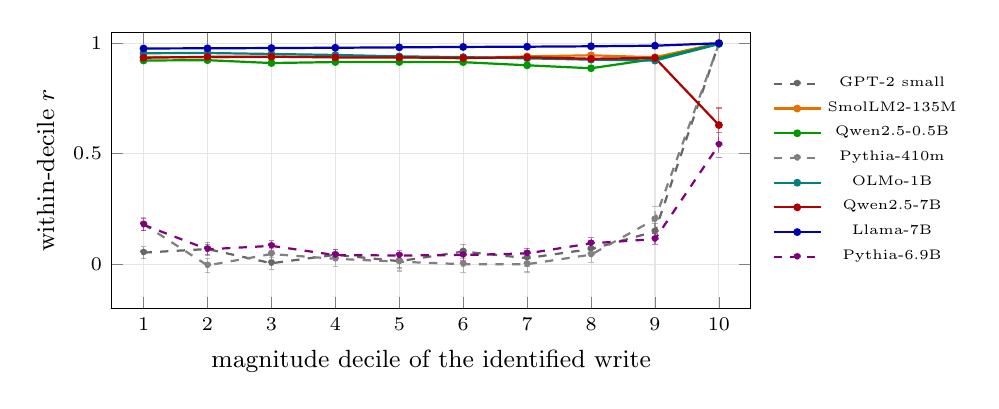
\begin{tikzpicture}\begin{axis}[width=0.8\linewidth, height=0.42\linewidth, xlabel={magnitude decile of the identified write}, ylabel={within-decile $r$}, xmin=0.5, xmax=10.5, ymin=-0.2, ymax=1.05, xtick={1,...,10}, grid=major, grid style={black!10}, legend style={font=\tiny, at={(1.02,0.5)}, anchor=west, draw=none}, tick label style={font=\scriptsize}, label style={font=\small}, error bars/y dir=both, error bars/y explicit]
\addplot[thick, dashed, color=black!60, mark=*, mark size=1pt, error bars/error bar style={opacity=0.5}] coordinates {(1,0.0528) +- (0,0.0276) (2,0.0690) +- (0,0.0305) (3,0.0048) +- (0,0.0267) (4,0.0430) +- (0,0.0248) (5,0.0142) +- (0,0.0311) (6,0.0576) +- (0,0.0325) (7,0.0280) +- (0,0.0357) (8,0.0690) +- (0,0.0301) (9,0.1484) +- (0,0.0368) (10,0.9998) +- (0,0.0000)};\addlegendentry{GPT-2 small}
\addplot[thick, color=orange!90!black, mark=*, mark size=1pt, error bars/error bar style={opacity=0.5}] coordinates {(1,0.9375) +- (0,0.0030) (2,0.9360) +- (0,0.0032) (3,0.9379) +- (0,0.0024) (4,0.9387) +- (0,0.0029) (5,0.9371) +- (0,0.0034) (6,0.9315) +- (0,0.0035) (7,0.9399) +- (0,0.0023) (8,0.9451) +- (0,0.0021) (9,0.9361) +- (0,0.0022) (10,0.9999) +- (0,0.0000)};\addlegendentry{SmolLM2-135M}
\addplot[thick, color=green!60!black, mark=*, mark size=1pt, error bars/error bar style={opacity=0.5}] coordinates {(1,0.9214) +- (0,0.0031) (2,0.9230) +- (0,0.0035) (3,0.9100) +- (0,0.0036) (4,0.9145) +- (0,0.0028) (5,0.9148) +- (0,0.0023) (6,0.9140) +- (0,0.0045) (7,0.8998) +- (0,0.0032) (8,0.8864) +- (0,0.0040) (9,0.9285) +- (0,0.0058) (10,0.9975) +- (0,0.0003)};\addlegendentry{Qwen2.5-0.5B}
\addplot[thick, dashed, color=gray, mark=*, mark size=1pt, error bars/error bar style={opacity=0.5}] coordinates {(1,0.1817) +- (0,0.0300) (2,-0.0050) +- (0,0.0328) (3,0.0464) +- (0,0.0252) (4,0.0249) +- (0,0.0346) (5,0.0118) +- (0,0.0421) (6,0.0004) +- (0,0.0356) (7,0.0005) +- (0,0.0351) (8,0.0437) +- (0,0.0340) (9,0.2037) +- (0,0.0590) (10,0.9963) +- (0,0.0005)};\addlegendentry{Pythia-410m}
\addplot[thick, color=teal, mark=*, mark size=1pt, error bars/error bar style={opacity=0.5}] coordinates {(1,0.9545) +- (0,0.0021) (2,0.9554) +- (0,0.0013) (3,0.9510) +- (0,0.0016) (4,0.9465) +- (0,0.0016) (5,0.9402) +- (0,0.0019) (6,0.9366) +- (0,0.0017) (7,0.9313) +- (0,0.0023) (8,0.9253) +- (0,0.0022) (9,0.9211) +- (0,0.0025) (10,0.9961) +- (0,0.0005)};\addlegendentry{OLMo-1B}
\addplot[thick, color=red!70!black, mark=*, mark size=1pt, error bars/error bar style={opacity=0.5}] coordinates {(1,0.9339) +- (0,0.0031) (2,0.9381) +- (0,0.0028) (3,0.9387) +- (0,0.0043) (4,0.9355) +- (0,0.0046) (5,0.9351) +- (0,0.0048) (6,0.9330) +- (0,0.0056) (7,0.9360) +- (0,0.0045) (8,0.9295) +- (0,0.0060) (9,0.9331) +- (0,0.0073) (10,0.6297) +- (0,0.0771)};\addlegendentry{Qwen2.5-7B}
\addplot[thick, color=blue!70!black, mark=*, mark size=1pt, error bars/error bar style={opacity=0.5}] coordinates {(1,0.9759) +- (0,0.0008) (2,0.9767) +- (0,0.0008) (3,0.9778) +- (0,0.0007) (4,0.9791) +- (0,0.0006) (5,0.9809) +- (0,0.0007) (6,0.9828) +- (0,0.0012) (7,0.9839) +- (0,0.0009) (8,0.9857) +- (0,0.0008) (9,0.9884) +- (0,0.0008) (10,0.9995) +- (0,0.0000)};\addlegendentry{Llama-7B}
\addplot[thick, dashed, color=violet, mark=*, mark size=1pt, error bars/error bar style={opacity=0.5}] coordinates {(1,0.1787) +- (0,0.0266) (2,0.0679) +- (0,0.0234) (3,0.0834) +- (0,0.0232) (4,0.0417) +- (0,0.0246) (5,0.0398) +- (0,0.0210) (6,0.0419) +- (0,0.0251) (7,0.0492) +- (0,0.0235) (8,0.0948) +- (0,0.0248) (9,0.1140) +- (0,0.0234) (10,0.5402) +- (0,0.0556)};\addlegendentry{Pythia-6.9B}
\end{axis}\end{tikzpicture}\caption{Within-decile correlation per model on the Pile sample, with 95\% bootstrap intervals as error bars. Solid lines are gated-MLP models, dashed non-gated.}\label{app:ci-decilefig-pile}\end{figure}
\begin{table}[H]\centering\scriptsize
\caption{The individual experiment scripts (8{,}192 states for the non-GPT-2 models, corpus-restricted embedding atoms) against the single-protocol sweep on WikiText-2 (32{,}768 states, full-vocabulary dictionaries), both over all states. Agreement within the intervals is the replication check; the remaining differences come from the token sample and the dictionary size.}\label{app:ci-old}
\begin{adjustbox}{max width=\linewidth}
\begin{tabular}{lrrrrrrrr}\toprule
Model & FVU@32, scripts & sweep & recall, scripts & sweep & $r$ id., scripts & sweep & $r$ unc., scripts & sweep \\ \midrule
GPT-2 small & 0.069 & 0.069 [0.068, 0.069] & 0.647 & 0.647 [0.637, 0.657] & 0.998 & 0.998 [0.998, 0.998] & 0.648 & 0.648 [0.648, 0.648] \\
SmolLM2-135M & 0.006 & 0.006 [0.006, 0.006] & 0.673 & 0.670 [0.661, 0.680] & 1.000 & 1.000 [1.000, 1.000] & 0.927 & 0.928 [0.927, 0.928] \\
Qwen2.5-0.5B & 0.018 & 0.017 [0.016, 0.017] & 0.458 & 0.459 [0.451, 0.467] & 0.994 & 0.994 [0.993, 0.994] & 0.556 & 0.551 [0.543, 0.559] \\
Pythia-410m & 0.051 & 0.050 [0.049, 0.051] & 0.470 & 0.481 [0.472, 0.490] & 0.978 & 0.980 [0.979, 0.981] & 0.450 & 0.452 [0.446, 0.455] \\
OLMo-1B & 0.018 & 0.019 [0.018, 0.019] & 0.703 & 0.693 [0.687, 0.699] & 0.996 & 0.997 [0.997, 0.998] & 0.971 & 0.971 [0.969, 0.972] \\
Qwen2.5-7B & 0.010 & 0.010 [0.009, 0.010] & 0.684 & 0.673 [0.663, 0.685] & 0.549 & 0.554 [0.506, 0.595] & 0.312 & 0.308 [0.271, 0.343] \\
Llama-7B & 0.088 & 0.089 [0.087, 0.090] & 0.980 & 0.981 [0.979, 0.983] & 0.999 & 0.999 [0.999, 0.999] & 0.998 & 0.998 [0.998, 0.998] \\
Pythia-6.9B & 0.309 & 0.310 [0.303, 0.315] & 0.808 & 0.787 [0.779, 0.795] & 0.522 & 0.539 [0.528, 0.551] & 0.412 & 0.424 [0.409, 0.439] \\
\bottomrule\end{tabular}\end{adjustbox}
\end{table}

\section{The Ceiling in Each Model, the Matched SAE Comparison and Sparsity at Matched Budgets}\label{app:z}
This section uses the states, dictionaries, centering and bootstrap of Appendix~\ref{app:ci}.
\subsection{Identification and survival in all models}\label{app:z3}
\texttt{exp\_z3\_ceiling} repeats the GPT-2 analysis of Table~\ref{app:survbins} and Table~\ref{app:auc} for the eight models on both corpora: each token's three dominant MLP writes (98,304 cases per model and corpus), their survival $s=(\mathbf{x}\cdot\mathbf{d})/c$ in the observed state, and whether OMP at $k=64$ places the write's atom in the support. Two further quantities decompose the misses. A miss is \emph{erased} if $s<0.25$, \emph{weakened} if $0.25\le s<0.75$, a \emph{twin} miss if the write is intact but an atom within $|\cos|\ge0.95$ of its atom sits in the support instead, and \emph{intact, unselected} otherwise. The GPT-2 row reproduces Table~\ref{app:survbins} exactly.
\begin{table}[H]\centering\scriptsize
\caption{Identification of the three dominant writes on WikiText-2 against their survival. Intact means $s\ge0.75$, erased $s<0.25$. Brackets are 95\% bootstrap intervals over sequences.}\label{app:z3-surv-wikitext}
\begin{adjustbox}{max width=\linewidth}
\begin{tabular}{lrrrrrrrr}\toprule
Model & gated & identified, all cases & share intact & identified, intact & share erased & identified, erased & AUC survival & AUC prominence \\ \midrule
GPT-2 small & no & 0.491 [0.484, 0.497] & 0.834 & 0.584 [0.577, 0.590] & 0.128 & 0.008 [0.007, 0.009] & 0.73 & 0.80 \\
SmolLM2-135M & yes & 0.494 [0.490, 0.497] & 0.761 & 0.614 [0.610, 0.618] & 0.089 & 0.015 [0.013, 0.018] & 0.81 & 0.86 \\
Qwen2.5-0.5B & yes & 0.349 [0.345, 0.353] & 0.527 & 0.550 [0.545, 0.556] & 0.104 & 0.004 [0.003, 0.006] & 0.83 & 0.92 \\
Pythia-410m & no & 0.365 [0.358, 0.371] & 0.762 & 0.465 [0.457, 0.471] & 0.080 & 0.003 [0.002, 0.004] & 0.84 & 0.91 \\
OLMo-1B & yes & 0.606 [0.602, 0.611] & 0.637 & 0.788 [0.782, 0.793] & 0.063 & 0.036 [0.030, 0.041] & 0.82 & 0.89 \\
Qwen2.5-7B & yes & 0.556 [0.547, 0.565] & 0.363 & 0.778 [0.770, 0.787] & 0.094 & 0.076 [0.067, 0.085] & 0.76 & 0.88 \\
Llama-7B & yes & 0.946 [0.944, 0.949] & 0.976 & 0.962 [0.960, 0.963] & 0.009 & 0.150 [0.122, 0.178] & 0.76 & 0.85 \\
Pythia-6.9B & no & 0.687 [0.680, 0.694] & 0.922 & 0.744 [0.737, 0.750] & 0.062 & 0.007 [0.005, 0.009] & 0.82 & 0.86 \\
\bottomrule\end{tabular}\end{adjustbox}
\end{table}
\begin{table}[H]\centering\scriptsize
\caption{Where the misses come from on WikiText-2: the share of missed dominant writes in each class (the four shares sum to one).}\label{app:z3-miss-wikitext}
\begin{adjustbox}{max width=\linewidth}
\begin{tabular}{lrrrrrr}\toprule
Model & miss rate & erased & weakened & twin in support & intact, unselected & cases with a twin in the support \\ \midrule
GPT-2 small & 0.509 & 0.25 [0.24, 0.26] & 0.07 [0.07, 0.07] & 0.00 [0.00, 0.00] & 0.68 [0.67, 0.69] & 0.2\% \\
SmolLM2-135M & 0.506 & 0.17 [0.17, 0.18] & 0.25 [0.24, 0.25] & 0.00 [0.00, 0.00] & 0.58 [0.57, 0.59] & 0.4\% \\
Qwen2.5-0.5B & 0.651 & 0.16 [0.15, 0.16] & 0.48 [0.47, 0.48] & 0.00 [0.00, 0.00] & 0.36 [0.35, 0.37] & 0.1\% \\
Pythia-410m & 0.635 & 0.13 [0.12, 0.13] & 0.23 [0.23, 0.24] & 0.01 [0.01, 0.01] & 0.64 [0.63, 0.64] & 0.3\% \\
OLMo-1B & 0.394 & 0.15 [0.15, 0.16] & 0.50 [0.49, 0.51] & 0.00 [0.00, 0.00] & 0.34 [0.33, 0.35] & 0.1\% \\
Qwen2.5-7B & 0.444 & 0.20 [0.19, 0.20] & 0.62 [0.61, 0.63] & 0.00 [0.00, 0.00] & 0.18 [0.17, 0.19] & 0.2\% \\
Llama-7B & 0.054 & 0.14 [0.12, 0.15] & 0.17 [0.16, 0.18] & 0.01 [0.01, 0.01] & 0.69 [0.67, 0.70] & 0.4\% \\
Pythia-6.9B & 0.313 & 0.20 [0.19, 0.21] & 0.05 [0.05, 0.05] & 0.00 [0.00, 0.00] & 0.75 [0.74, 0.76] & 0.0\% \\
\bottomrule\end{tabular}\end{adjustbox}
\end{table}
\begin{table}[H]\centering\scriptsize
\caption{OMP identification rate by survival bin on WikiText-2 (the six bins of Figure~\ref{fig:fvu}).}\label{app:z3-bins-wikitext}
\begin{adjustbox}{max width=\linewidth}
\begin{tabular}{lrrrrrr}\toprule
Model & $s<0$ & $[0,0.25)$ & $[0.25,0.5)$ & $[0.5,0.75)$ & $[0.75,1.25)$ & $s\ge1.25$ \\ \midrule
GPT-2 small & 0.01 & 0.01 & 0.04 & 0.11 & 0.36 & 0.62 \\
SmolLM2-135M & 0.01 & 0.04 & 0.08 & 0.22 & 0.38 & 0.71 \\
Qwen2.5-0.5B & 0.00 & 0.01 & 0.10 & 0.20 & 0.36 & 0.73 \\
Pythia-410m & 0.00 & 0.00 & 0.02 & 0.09 & 0.22 & 0.62 \\
OLMo-1B & 0.06 & 0.02 & 0.15 & 0.45 & 0.72 & 0.88 \\
Qwen2.5-7B & 0.03 & 0.08 & 0.38 & 0.60 & 0.75 & 0.85 \\
Llama-7B & 0.15 & 0.15 & 0.26 & 0.51 & 0.84 & 0.97 \\
Pythia-6.9B & 0.01 & 0.01 & 0.02 & 0.03 & 0.10 & 0.77 \\
\bottomrule\end{tabular}\end{adjustbox}
\end{table}
\begin{figure}[H]\centering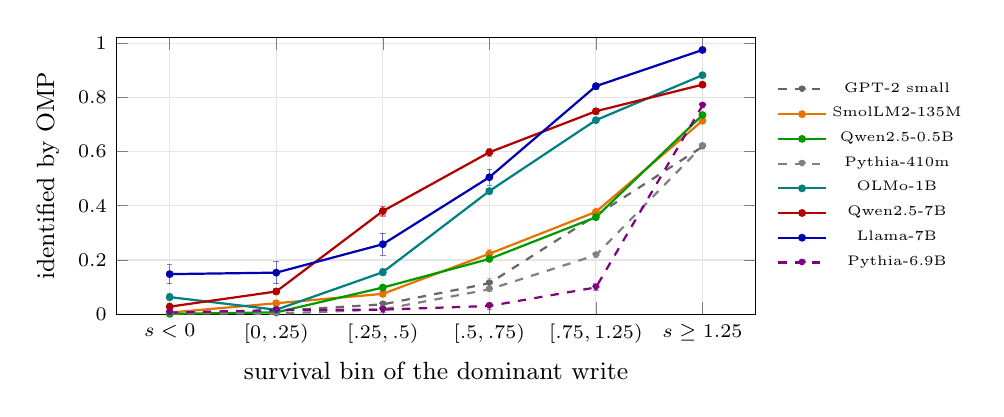
\begin{tikzpicture}\begin{axis}[width=0.8\linewidth, height=0.42\linewidth, xlabel={survival bin of the dominant write}, ylabel={identified by OMP}, xmin=0.5, xmax=6.5, ymin=0, ymax=1.02, xtick={1,...,6}, xticklabels={{$s<0$},{$[0,.25)$},{$[.25,.5)$},{$[.5,.75)$},{$[.75,1.25)$},{$s\ge1.25$}}, grid=major, grid style={black!10}, legend style={font=\tiny, at={(1.02,0.5)}, anchor=west, draw=none}, tick label style={font=\scriptsize}, label style={font=\small}, error bars/y dir=both, error bars/y explicit]
\addplot[thick, dashed, color=black!60, mark=*, mark size=1pt, error bars/error bar style={opacity=0.5}] coordinates {(1,0.0074) +- (0,0.0013) (2,0.0122) +- (0,0.0058) (3,0.0362) +- (0,0.0101) (4,0.1141) +- (0,0.0166) (5,0.3644) +- (0,0.0106) (6,0.6178) +- (0,0.0066)};\addlegendentry{GPT-2 small}
\addplot[thick, color=orange!90!black, mark=*, mark size=1pt, error bars/error bar style={opacity=0.5}] coordinates {(1,0.0058) +- (0,0.0018) (2,0.0404) +- (0,0.0087) (3,0.0750) +- (0,0.0083) (4,0.2229) +- (0,0.0152) (5,0.3774) +- (0,0.0100) (6,0.7137) +- (0,0.0057)};\addlegendentry{SmolLM2-135M}
\addplot[thick, color=green!60!black, mark=*, mark size=1pt, error bars/error bar style={opacity=0.5}] coordinates {(1,0.0012) +- (0,0.0012) (2,0.0067) +- (0,0.0025) (3,0.0982) +- (0,0.0088) (4,0.2038) +- (0,0.0088) (5,0.3578) +- (0,0.0066) (6,0.7346) +- (0,0.0074)};\addlegendentry{Qwen2.5-0.5B}
\addplot[thick, dashed, color=gray, mark=*, mark size=1pt, error bars/error bar style={opacity=0.5}] coordinates {(1,0.0039) +- (0,0.0018) (2,0.0015) +- (0,0.0015) (3,0.0179) +- (0,0.0031) (4,0.0917) +- (0,0.0062) (5,0.2178) +- (0,0.0081) (6,0.6207) +- (0,0.0097)};\addlegendentry{Pythia-410m}
\addplot[thick, color=teal, mark=*, mark size=1pt, error bars/error bar style={opacity=0.5}] coordinates {(1,0.0630) +- (0,0.0116) (2,0.0164) +- (0,0.0052) (3,0.1548) +- (0,0.0121) (4,0.4543) +- (0,0.0110) (5,0.7158) +- (0,0.0074) (6,0.8817) +- (0,0.0051)};\addlegendentry{OLMo-1B}
\addplot[thick, color=red!70!black, mark=*, mark size=1pt, error bars/error bar style={opacity=0.5}] coordinates {(1,0.0277) +- (0,0.0110) (2,0.0837) +- (0,0.0097) (3,0.3803) +- (0,0.0182) (4,0.5972) +- (0,0.0142) (5,0.7487) +- (0,0.0105) (6,0.8468) +- (0,0.0073)};\addlegendentry{Qwen2.5-7B}
\addplot[thick, color=blue!70!black, mark=*, mark size=1pt, error bars/error bar style={opacity=0.5}] coordinates {(1,0.1478) +- (0,0.0349) (2,0.1532) +- (0,0.0413) (3,0.2581) +- (0,0.0411) (4,0.5052) +- (0,0.0290) (5,0.8413) +- (0,0.0108) (6,0.9748) +- (0,0.0014)};\addlegendentry{Llama-7B}
\addplot[thick, dashed, color=violet, mark=*, mark size=1pt, error bars/error bar style={opacity=0.5}] coordinates {(1,0.0060) +- (0,0.0021) (2,0.0149) +- (0,0.0090) (3,0.0168) +- (0,0.0099) (4,0.0303) +- (0,0.0131) (5,0.0987) +- (0,0.0125) (6,0.7697) +- (0,0.0057)};\addlegendentry{Pythia-6.9B}
\end{axis}\end{tikzpicture}\caption{Identification against survival for all eight models on WikiText-2. Solid lines are gated-MLP models, dashed non-gated.}\label{app:z3-fig-wikitext}\end{figure}
\begin{table}[H]\centering\scriptsize
\caption{Identification of the three dominant writes on the Pile sample against their survival. Intact means $s\ge0.75$, erased $s<0.25$. Brackets are 95\% bootstrap intervals over sequences.}\label{app:z3-surv-pile}
\begin{adjustbox}{max width=\linewidth}
\begin{tabular}{lrrrrrrrr}\toprule
Model & gated & identified, all cases & share intact & identified, intact & share erased & identified, erased & AUC survival & AUC prominence \\ \midrule
GPT-2 small & no & 0.439 [0.423, 0.454] & 0.765 & 0.571 [0.560, 0.581] & 0.187 & 0.007 [0.005, 0.009] & 0.80 & 0.83 \\
SmolLM2-135M & yes & 0.489 [0.479, 0.497] & 0.794 & 0.594 [0.587, 0.601] & 0.082 & 0.010 [0.008, 0.012] & 0.81 & 0.88 \\
Qwen2.5-0.5B & yes & 0.365 [0.355, 0.375] & 0.573 & 0.551 [0.544, 0.559] & 0.093 & 0.002 [0.001, 0.003] & 0.84 & 0.92 \\
Pythia-410m & no & 0.346 [0.337, 0.353] & 0.735 & 0.454 [0.446, 0.461] & 0.084 & 0.004 [0.002, 0.008] & 0.83 & 0.91 \\
OLMo-1B & yes & 0.639 [0.632, 0.647] & 0.704 & 0.778 [0.771, 0.786] & 0.043 & 0.027 [0.021, 0.033] & 0.79 & 0.87 \\
Qwen2.5-7B & yes & 0.578 [0.567, 0.588] & 0.475 & 0.761 [0.750, 0.772] & 0.069 & 0.068 [0.060, 0.077] & 0.75 & 0.87 \\
Llama-7B & yes & 0.948 [0.944, 0.951] & 0.977 & 0.962 [0.960, 0.964] & 0.008 & 0.112 [0.093, 0.134] & 0.75 & 0.84 \\
Pythia-6.9B & no & 0.669 [0.656, 0.681] & 0.915 & 0.730 [0.718, 0.741] & 0.072 & 0.010 [0.007, 0.013] & 0.80 & 0.80 \\
\bottomrule\end{tabular}\end{adjustbox}
\end{table}
\begin{table}[H]\centering\scriptsize
\caption{Where the misses come from on the Pile sample: the share of missed dominant writes in each class (the four shares sum to one).}\label{app:z3-miss-pile}
\begin{adjustbox}{max width=\linewidth}
\begin{tabular}{lrrrrrr}\toprule
Model & miss rate & erased & weakened & twin in support & intact, unselected & cases with a twin in the support \\ \midrule
GPT-2 small & 0.561 & 0.33 [0.30, 0.37] & 0.08 [0.08, 0.09] & 0.00 [0.00, 0.00] & 0.58 [0.55, 0.61] & 0.3\% \\
SmolLM2-135M & 0.511 & 0.16 [0.15, 0.17] & 0.21 [0.20, 0.22] & 0.00 [0.00, 0.00] & 0.63 [0.62, 0.64] & 0.3\% \\
Qwen2.5-0.5B & 0.635 & 0.15 [0.14, 0.15] & 0.45 [0.43, 0.46] & 0.00 [0.00, 0.00] & 0.40 [0.39, 0.42] & 0.1\% \\
Pythia-410m & 0.654 & 0.13 [0.12, 0.14] & 0.26 [0.25, 0.27] & 0.01 [0.00, 0.01] & 0.61 [0.60, 0.62] & 0.3\% \\
OLMo-1B & 0.361 & 0.12 [0.11, 0.12] & 0.45 [0.44, 0.46] & 0.00 [0.00, 0.00] & 0.43 [0.41, 0.44] & 0.1\% \\
Qwen2.5-7B & 0.422 & 0.15 [0.15, 0.16] & 0.58 [0.57, 0.59] & 0.00 [0.00, 0.00] & 0.26 [0.25, 0.28] & 0.2\% \\
Llama-7B & 0.052 & 0.14 [0.13, 0.16] & 0.15 [0.14, 0.17] & 0.01 [0.01, 0.01] & 0.70 [0.67, 0.72] & 0.4\% \\
Pythia-6.9B & 0.331 & 0.22 [0.20, 0.23] & 0.04 [0.04, 0.04] & 0.00 [0.00, 0.00] & 0.74 [0.73, 0.76] & 0.1\% \\
\bottomrule\end{tabular}\end{adjustbox}
\end{table}
\begin{table}[H]\centering\scriptsize
\caption{OMP identification rate by survival bin on the Pile sample (the six bins of Figure~\ref{fig:fvu}).}\label{app:z3-bins-pile}
\begin{adjustbox}{max width=\linewidth}
\begin{tabular}{lrrrrrr}\toprule
Model & $s<0$ & $[0,0.25)$ & $[0.25,0.5)$ & $[0.5,0.75)$ & $[0.75,1.25)$ & $s\ge1.25$ \\ \midrule
GPT-2 small & 0.01 & 0.00 & 0.01 & 0.05 & 0.24 & 0.62 \\
SmolLM2-135M & 0.00 & 0.02 & 0.08 & 0.16 & 0.33 & 0.70 \\
Qwen2.5-0.5B & 0.00 & 0.00 & 0.08 & 0.20 & 0.36 & 0.74 \\
Pythia-410m & 0.00 & 0.00 & 0.01 & 0.09 & 0.23 & 0.61 \\
OLMo-1B & 0.02 & 0.03 & 0.17 & 0.45 & 0.71 & 0.86 \\
Qwen2.5-7B & 0.06 & 0.07 & 0.35 & 0.55 & 0.72 & 0.83 \\
Llama-7B & 0.08 & 0.17 & 0.37 & 0.51 & 0.81 & 0.97 \\
Pythia-6.9B & 0.01 & 0.01 & 0.03 & 0.05 & 0.11 & 0.75 \\
\bottomrule\end{tabular}\end{adjustbox}
\end{table}
\begin{figure}[H]\centering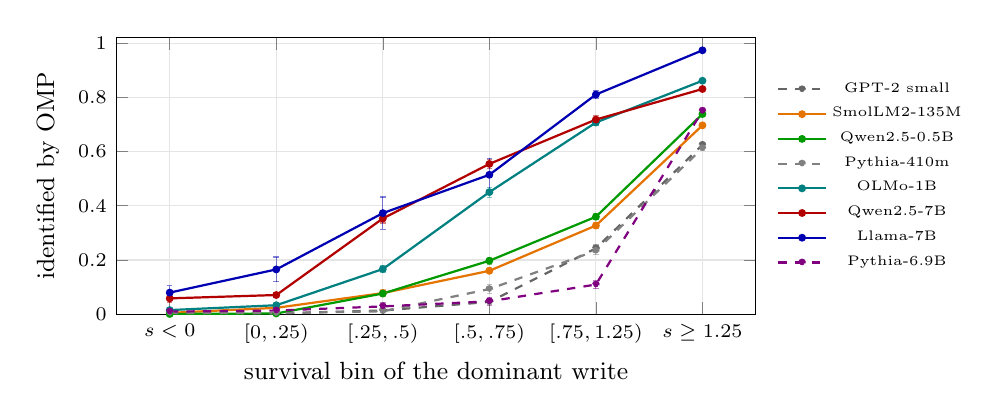
\begin{tikzpicture}\begin{axis}[width=0.8\linewidth, height=0.42\linewidth, xlabel={survival bin of the dominant write}, ylabel={identified by OMP}, xmin=0.5, xmax=6.5, ymin=0, ymax=1.02, xtick={1,...,6}, xticklabels={{$s<0$},{$[0,.25)$},{$[.25,.5)$},{$[.5,.75)$},{$[.75,1.25)$},{$s\ge1.25$}}, grid=major, grid style={black!10}, legend style={font=\tiny, at={(1.02,0.5)}, anchor=west, draw=none}, tick label style={font=\scriptsize}, label style={font=\small}, error bars/y dir=both, error bars/y explicit]
\addplot[thick, dashed, color=black!60, mark=*, mark size=1pt, error bars/error bar style={opacity=0.5}] coordinates {(1,0.0074) +- (0,0.0019) (2,0.0028) +- (0,0.0023) (3,0.0136) +- (0,0.0060) (4,0.0453) +- (0,0.0102) (5,0.2429) +- (0,0.0125) (6,0.6247) +- (0,0.0097)};\addlegendentry{GPT-2 small}
\addplot[thick, color=orange!90!black, mark=*, mark size=1pt, error bars/error bar style={opacity=0.5}] coordinates {(1,0.0048) +- (0,0.0018) (2,0.0234) +- (0,0.0072) (3,0.0778) +- (0,0.0116) (4,0.1600) +- (0,0.0111) (5,0.3270) +- (0,0.0102) (6,0.6967) +- (0,0.0071)};\addlegendentry{SmolLM2-135M}
\addplot[thick, color=green!60!black, mark=*, mark size=1pt, error bars/error bar style={opacity=0.5}] coordinates {(1,0.0008) +- (0,0.0008) (2,0.0025) +- (0,0.0014) (3,0.0762) +- (0,0.0085) (4,0.1971) +- (0,0.0128) (5,0.3594) +- (0,0.0108) (6,0.7383) +- (0,0.0077)};\addlegendentry{Qwen2.5-0.5B}
\addplot[thick, dashed, color=gray, mark=*, mark size=1pt, error bars/error bar style={opacity=0.5}] coordinates {(1,0.0048) +- (0,0.0050) (2,0.0037) +- (0,0.0026) (3,0.0107) +- (0,0.0024) (4,0.0926) +- (0,0.0157) (5,0.2339) +- (0,0.0150) (6,0.6123) +- (0,0.0085)};\addlegendentry{Pythia-410m}
\addplot[thick, color=teal, mark=*, mark size=1pt, error bars/error bar style={opacity=0.5}] coordinates {(1,0.0151) +- (0,0.0081) (2,0.0330) +- (0,0.0074) (3,0.1664) +- (0,0.0120) (4,0.4503) +- (0,0.0183) (5,0.7072) +- (0,0.0107) (6,0.8613) +- (0,0.0070)};\addlegendentry{OLMo-1B}
\addplot[thick, color=red!70!black, mark=*, mark size=1pt, error bars/error bar style={opacity=0.5}] coordinates {(1,0.0583) +- (0,0.0153) (2,0.0707) +- (0,0.0097) (3,0.3530) +- (0,0.0167) (4,0.5544) +- (0,0.0170) (5,0.7180) +- (0,0.0146) (6,0.8308) +- (0,0.0107)};\addlegendentry{Qwen2.5-7B}
\addplot[thick, color=blue!70!black, mark=*, mark size=1pt, error bars/error bar style={opacity=0.5}] coordinates {(1,0.0796) +- (0,0.0247) (2,0.1651) +- (0,0.0458) (3,0.3728) +- (0,0.0596) (4,0.5143) +- (0,0.0604) (5,0.8104) +- (0,0.0148) (6,0.9735) +- (0,0.0014)};\addlegendentry{Llama-7B}
\addplot[thick, dashed, color=violet, mark=*, mark size=1pt, error bars/error bar style={opacity=0.5}] coordinates {(1,0.0096) +- (0,0.0028) (2,0.0133) +- (0,0.0105) (3,0.0287) +- (0,0.0143) (4,0.0475) +- (0,0.0150) (5,0.1093) +- (0,0.0148) (6,0.7500) +- (0,0.0121)};\addlegendentry{Pythia-6.9B}
\end{axis}\end{tikzpicture}\caption{Identification against survival for all eight models on the Pile sample. Solid lines are gated-MLP models, dashed non-gated.}\label{app:z3-fig-pile}\end{figure}
\begin{table}[H]\centering\scriptsize
\caption{Composition of the $k=64$ support by atom type on WikiText-2.}\label{app:z3-support}
\begin{adjustbox}{max width=\linewidth}
\begin{tabular}{lrrrr}\toprule
Model & embedding & MLP & attention & bias \\ \midrule
GPT-2 small & 17.1\% & 62.1\% & 20.7\% & 0.1\% \\
SmolLM2-135M & 8.5\% & 71.4\% & 20.1\% & 0.0\% \\
Qwen2.5-0.5B & 36.4\% & 54.5\% & 9.1\% & 0.0\% \\
Pythia-410m & 32.8\% & 53.4\% & 13.8\% & 0.0\% \\
OLMo-1B & 16.1\% & 70.4\% & 13.5\% & 0.0\% \\
Qwen2.5-7B & 6.8\% & 80.5\% & 12.7\% & 0.0\% \\
Llama-7B & 2.0\% & 76.9\% & 21.1\% & 0.0\% \\
Pythia-6.9B & 3.9\% & 70.9\% & 25.2\% & 0.0\% \\
\bottomrule\end{tabular}\end{adjustbox}
\end{table}
\subsection{The SAE comparison on identical states}\label{app:z4}
\texttt{exp\_z4\_sae} evaluates the residual-stream SAEs of \citet{bloom2024} from their published weights and the weight dictionary on the same GPT-2 states in four cells: WikiText-2 with 512-token contexts (the paper's states) and OpenWebText with 128-token contexts and a leading beginning-of-text token (the SAEs' training convention), each at the state after block 5 (the input of block 6, where the SAE named \texttt{blocks.6} was trained) and after block 6 (the paper's layer, where \texttt{blocks.7} was trained). The SAEs read the residual stream in the TransformerLens frame, in which each state is centered over the model dimension, and the states are centered the same way before encoding. $L_0$ is the SAE's mean number of active features over the typical states; the weight dictionary is run at $k=32$, $k=64$ and at $k$ equal to that $L_0$. FVU is over the typical states with one denominator per cell for both methods (for GPT-2 the sink states are exactly the first positions), and $\Delta$CE is the change in next-token cross-entropy over all positions when the reconstruction replaces the state in the forward pass. On the 512-token states the SAE fails past position 127, which it never saw in training, so the two 128-token cells are the matched comparison.
\begin{table}[H]\centering\scriptsize
\caption{The trained SAE and the weight dictionary on identical GPT-2 states. Brackets are 95\% bootstrap intervals over sequences (64 WikiText-2 sequences, 256 OpenWebText documents).}\label{app:z4-table}
\begin{adjustbox}{max width=\linewidth}
\begin{tabular}{llrlrrr}\toprule
Corpus, context & state & clean CE & method & $L_0$ or $k$ & FVU, typical states & $\Delta$CE \\ \midrule
WikiText-2, 512 & after block 5 & 3.647 & SAE & 161.6 & 2.878 [2.757, 3.006] & 1.443 [1.390, 1.492] \\
 &  &  & weight dictionary & 32 & 0.325 [0.324, 0.327] & 0.521 [0.495, 0.548] \\
 &  &  & weight dictionary & 64 & 0.174 [0.173, 0.174] & 0.161 [0.150, 0.171] \\
 &  &  & weight dictionary & 162 & 0.023 [0.023, 0.023] & 0.013 [0.011, 0.015] \\
WikiText-2, 512 & after block 6 & 3.647 & SAE & 161.4 & 1.480 [1.422, 1.540] & 1.088 [1.044, 1.131] \\
 &  &  & weight dictionary & 32 & 0.338 [0.337, 0.340] & 0.551 [0.522, 0.581] \\
 &  &  & weight dictionary & 64 & 0.179 [0.179, 0.180] & 0.178 [0.167, 0.189] \\
 &  &  & weight dictionary & 161 & 0.024 [0.024, 0.024] & 0.015 [0.013, 0.017] \\
OpenWebText, 128 & after block 5 & 3.323 & SAE & 51.2 & 0.109 [0.107, 0.111] & 0.144 [0.135, 0.155] \\
 &  &  & weight dictionary & 32 & 0.307 [0.306, 0.308] & 0.428 [0.411, 0.448] \\
 &  &  & weight dictionary & 51 & 0.210 [0.209, 0.211] & 0.188 [0.179, 0.197] \\
 &  &  & weight dictionary & 64 & 0.163 [0.162, 0.164] & 0.125 [0.118, 0.132] \\
OpenWebText, 128 & after block 6 & 3.323 & SAE & 58.8 & 0.121 [0.119, 0.123] & 0.155 [0.145, 0.165] \\
 &  &  & weight dictionary & 32 & 0.320 [0.319, 0.321] & 0.477 [0.460, 0.497] \\
 &  &  & weight dictionary & 59 & 0.187 [0.186, 0.187] & 0.172 [0.165, 0.181] \\
 &  &  & weight dictionary & 64 & 0.169 [0.169, 0.170] & 0.146 [0.138, 0.154] \\
\bottomrule\end{tabular}\end{adjustbox}
\end{table}
\subsection{Sparsity at matched budgets}\label{app:z5}
\texttt{exp\_z5\_kcurve} sweeps $k$ for the weight dictionary and its rotation on 8,192 WikiText-2 states per model (the first 16 evaluation sequences of the sweep), reading the FVU at $k=4$ to $256$ and at the matched budgets $k=d/16$ and $k=d/12$, so that models of different width are compared at the same fraction of their dimension. The table and the figure are over the typical states.
\begin{table}[H]\centering\scriptsize
\caption{FVU of the typical states at a fixed budget of 32 atoms, at budgets matched to the width, and at 256 atoms.}\label{app:z5-table}
\begin{adjustbox}{max width=\linewidth}
\begin{tabular}{lrrrrrrrrrrr}\toprule
Model & $d$ & weight, $k=32$ & rotated, $k=32$ & $k=d/16$ & weight & rotated & $k=d/12$ & weight & rotated & weight, $k=256$ & rotated, $k=256$ \\ \midrule
GPT-2 small & 768 & 0.334 & 0.530 & 48 & 0.243 & 0.391 & 64 & 0.177 & 0.288 & 0.002 & 0.004 \\
SmolLM2-135M & 576 & 0.270 & 0.421 & 36 & 0.242 & 0.379 & 48 & 0.175 & 0.276 & 0.000 & 0.000 \\
Qwen2.5-0.5B & 896 & 0.407 & 0.527 & 56 & 0.255 & 0.330 & 74 & 0.180 & 0.231 & 0.003 & 0.004 \\
Pythia-410m & 1024 & 0.501 & 0.592 & 64 & 0.301 & 0.359 & 85 & 0.216 & 0.257 & 0.010 & 0.013 \\
OLMo-1B & 2048 & 0.564 & 0.773 & 128 & 0.269 & 0.382 & 170 & 0.197 & 0.280 & 0.102 & 0.145 \\
Qwen2.5-7B & 3584 & 0.543 & 0.847 & 224 & 0.210 & 0.351 & 298 & 0.150 & 0.249 & 0.182 & 0.303 \\
Llama-7B & 4096 & 0.621 & 0.872 & 256 & 0.245 & 0.380 & 341 & 0.178 & 0.277 & 0.245 & 0.380 \\
Pythia-6.9B & 4096 & 0.707 & 0.868 & 256 & 0.279 & 0.363 & 341 & 0.199 & 0.260 & 0.279 & 0.363 \\
\bottomrule\end{tabular}\end{adjustbox}
\end{table}
\begin{figure}[H]\centering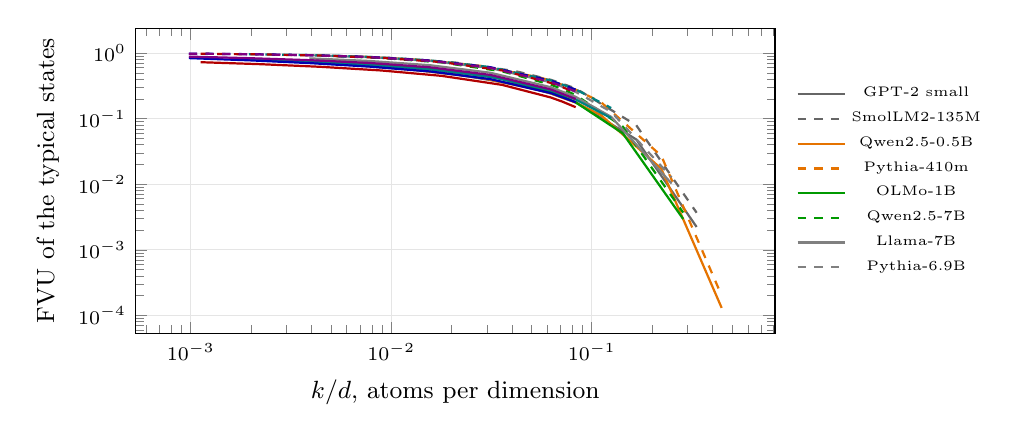
\begin{tikzpicture}\begin{axis}[width=0.8\linewidth, height=0.45\linewidth, xmode=log, ymode=log, xlabel={$k/d$, atoms per dimension}, ylabel={FVU of the typical states}, grid=major, grid style={black!10}, legend style={font=\tiny, at={(1.02,0.5)}, anchor=west, draw=none}, tick label style={font=\scriptsize}, label style={font=\small}]
\addplot[thick, color=black!60, mark=none] coordinates {(0.00521,0.70182) (0.01042,0.59594) (0.02083,0.47543) (0.04167,0.33432) (0.06250,0.24267) (0.08333,0.17722) (0.16667,0.04821) (0.33333,0.00223)};\addlegendentry{GPT-2 small}
\addplot[thick, dashed, color=black!60, mark=none] coordinates {(0.00521,0.91273) (0.01042,0.84044) (0.02083,0.71841) (0.04167,0.52985) (0.06250,0.39147) (0.08333,0.28833) (0.16667,0.07938) (0.33333,0.00368)};
\addplot[thick, color=orange!90!black, mark=none] coordinates {(0.00694,0.64552) (0.01389,0.54337) (0.02778,0.42082) (0.05556,0.26965) (0.06250,0.24208) (0.08333,0.17527) (0.11111,0.11340) (0.22222,0.01721) (0.44444,0.00013)};\addlegendentry{SmolLM2-135M}
\addplot[thick, dashed, color=orange!90!black, mark=none] coordinates {(0.00694,0.88485) (0.01389,0.79223) (0.02778,0.64034) (0.05556,0.42137) (0.06250,0.37931) (0.08333,0.27592) (0.11111,0.17888) (0.22222,0.02713) (0.44444,0.00020)};
\addplot[thick, color=green!60!black, mark=none] coordinates {(0.00446,0.76610) (0.00893,0.67655) (0.01786,0.56148) (0.03571,0.40654) (0.06250,0.25531) (0.07143,0.21853) (0.08259,0.17964) (0.14286,0.05966) (0.28571,0.00295)};\addlegendentry{Qwen2.5-0.5B}
\addplot[thick, dashed, color=green!60!black, mark=none] coordinates {(0.00446,0.91490) (0.00893,0.84295) (0.01786,0.71948) (0.03571,0.52720) (0.06250,0.33011) (0.07143,0.28188) (0.08259,0.23100) (0.14286,0.07562) (0.28571,0.00369)};
\addplot[thick, color=gray, mark=none] coordinates {(0.00391,0.83108) (0.00781,0.75796) (0.01562,0.65336) (0.03125,0.50108) (0.06250,0.30149) (0.08301,0.21573) (0.12500,0.10653) (0.25000,0.01027)};\addlegendentry{Pythia-410m}
\addplot[thick, dashed, color=gray, mark=none] coordinates {(0.00391,0.92772) (0.00781,0.86685) (0.01562,0.76126) (0.03125,0.59174) (0.06250,0.35859) (0.08301,0.25691) (0.12500,0.12712) (0.25000,0.01278)};
\addplot[thick, color=teal, mark=none] coordinates {(0.00195,0.81035) (0.00391,0.73906) (0.00781,0.65963) (0.01562,0.56372) (0.03125,0.43529) (0.06250,0.26923) (0.08301,0.19676) (0.12500,0.10192)};\addlegendentry{OLMo-1B}
\addplot[thick, dashed, color=teal, mark=none] coordinates {(0.00195,0.96293) (0.00391,0.93095) (0.00781,0.87330) (0.01562,0.77300) (0.03125,0.61051) (0.06250,0.38237) (0.08301,0.28012) (0.12500,0.14530)};
\addplot[thick, color=red!70!black, mark=none] coordinates {(0.00112,0.72614) (0.00223,0.67718) (0.00446,0.61711) (0.00893,0.54290) (0.01786,0.44912) (0.03571,0.32752) (0.06250,0.21035) (0.07143,0.18162) (0.08315,0.14961)};\addlegendentry{Qwen2.5-7B}
\addplot[thick, dashed, color=red!70!black, mark=none] coordinates {(0.00112,0.97601) (0.00223,0.95493) (0.00446,0.91628) (0.00893,0.84715) (0.01786,0.72894) (0.03571,0.54395) (0.06250,0.35087) (0.07143,0.30268) (0.08315,0.24890)};
\addplot[thick, color=blue!70!black, mark=none] coordinates {(0.00098,0.83841) (0.00195,0.77576) (0.00391,0.70340) (0.00781,0.62135) (0.01562,0.52419) (0.03125,0.40005) (0.06250,0.24508) (0.08325,0.17775)};\addlegendentry{Llama-7B}
\addplot[thick, dashed, color=blue!70!black, mark=none] coordinates {(0.00098,0.97997) (0.00195,0.96244) (0.00391,0.93023) (0.00781,0.87225) (0.01562,0.77151) (0.03125,0.60857) (0.06250,0.38024) (0.08325,0.27691)};
\addplot[thick, color=violet, mark=none] coordinates {(0.00098,0.88298) (0.00195,0.83674) (0.00391,0.77975) (0.00781,0.70718) (0.01562,0.60684) (0.03125,0.46405) (0.06250,0.27925) (0.08325,0.19927)};\addlegendentry{Pythia-6.9B}
\addplot[thick, dashed, color=violet, mark=none] coordinates {(0.00098,0.97945) (0.00195,0.96137) (0.00391,0.92807) (0.00781,0.86805) (0.01562,0.76386) (0.03125,0.59590) (0.06250,0.36345) (0.08325,0.26021)};
\end{axis}\end{tikzpicture}\caption{Reconstruction of the typical states against the relative budget $k/d$ for the weight dictionary (solid) and its rotation (dashed), eight models on WikiText-2.}\label{app:z5-fig}\end{figure}
\subsection{The GPT-2 sparsity sweep and the provenance null on typical states}\label{app:z-gpt2}
Tables~\ref{app:z-gpt2-typical} and~\ref{app:z-gpt2-all} give the GPT-2 sparsity sweep and the provenance controls of Section~\ref{sec:recon} over the typical states and over all states, from the per-token residuals of \texttt{exp\_a\_wdd} and \texttt{exp\_d\_provenance}. The sink states are 64 of the 32{,}768 layer-6 states and carry 79.7\% of the variance. The main text quotes the typical-state rows; Appendix~\ref{app:recon} has the all-state sweep with the spliced-in cross-entropies.
\begin{table}[H]\centering\scriptsize
\caption{GPT-2 layer 6, FVU against sparsity over the typical states.}\label{app:z-gpt2-typical}
\begin{adjustbox}{max width=\linewidth}
\begin{tabular}{lrrrrr}\toprule
Dictionary & $k=4$ & $k=8$ & $k=16$ & $k=32$ & $k=64$ \\ \midrule
weight dictionary & 0.707 & 0.601 & 0.481 & 0.338 & 0.179 \\
weight dictionary, no centering & 0.896 & 0.727 & 0.562 & 0.390 & 0.206 \\
sampled-activation dictionary & 0.286 & 0.222 & 0.166 & 0.113 & 0.063 \\
PCA, best $k$ per state & 0.774 & 0.684 & 0.582 & 0.469 & 0.341 \\
random directions & 0.908 & 0.832 & 0.701 & 0.500 & 0.251 \\
rotated weight dictionary & 0.912 & 0.840 & 0.718 & 0.529 & 0.288 \\
correct dictionary, subsampled to the null size & 0.723 & 0.621 & 0.502 & 0.358 & 0.194 \\
provenance null: atoms from blocks 7 to 11 & 0.810 & 0.723 & 0.608 & 0.449 & 0.252 \\
\bottomrule\end{tabular}\end{adjustbox}
\end{table}
\begin{table}[H]\centering\scriptsize
\caption{GPT-2 layer 6, FVU against sparsity over the all states.}\label{app:z-gpt2-all}
\begin{adjustbox}{max width=\linewidth}
\begin{tabular}{lrrrrr}\toprule
Dictionary & $k=4$ & $k=8$ & $k=16$ & $k=32$ & $k=64$ \\ \midrule
weight dictionary & 0.144 & 0.122 & 0.098 & 0.069 & 0.036 \\
weight dictionary, no centering & 0.182 & 0.148 & 0.114 & 0.079 & 0.042 \\
sampled-activation dictionary & 0.058 & 0.045 & 0.034 & 0.023 & 0.013 \\
PCA, best $k$ per state & 0.157 & 0.139 & 0.118 & 0.095 & 0.069 \\
random directions & 0.911 & 0.833 & 0.700 & 0.501 & 0.252 \\
rotated weight dictionary & 0.924 & 0.855 & 0.737 & 0.549 & 0.299 \\
correct dictionary, subsampled to the null size & 0.150 & 0.128 & 0.102 & 0.073 & 0.040 \\
provenance null: atoms from blocks 7 to 11 & 0.165 & 0.147 & 0.123 & 0.091 & 0.051 \\
\bottomrule\end{tabular}\end{adjustbox}
\end{table}
\subsection{What the support contains}\label{app:z6}
\texttt{exp\_z6\_selected} scores the other direction of attribution: every atom that OMP places in the $k=64$ support rather than the three dominant ledger writes. A selected MLP atom is a \emph{real} write when the ledger coefficient of its neuron at that token is at least 5\% of the token's largest write; otherwise the pursuit has spent an atom on a write that is not there. The table gives the composition of the support on the typical states, the share of selected MLP atoms that are real, the sign agreement and the median relative error of their recovered coefficients, and the share of the recovered MLP coefficient mass that sits on spurious atoms. The last columns compare OMP with a least-squares refit on the three true atoms on the same identified cases, which the main text's oracle could not do.
\begin{table}[H]\centering\scriptsize
\caption{The $k=64$ support on WikiText-2, typical states. The first three columns are the composition of the support by atom type; the next five describe the selected MLP atoms; the last four compare OMP and the true-top-3 refit on the same identified dominant writes.}\label{app:z6-wikitext}
\begin{adjustbox}{max width=\linewidth}
\begin{tabular}{lrrrrrrrrrrrr}\toprule
Model & MLP & attn. & emb. & real share of selected MLP atoms & sign & rel. error & ratio & spurious mass & $r$ OMP & $r$ refit & rel. err. OMP & rel. err. refit \\ \midrule
GPT-2 small & 62\% & 21\% & 17\% & 0.35 [0.34, 0.35] & 88.5\% & 1.55 & 2.07 & 57\% & 0.582 & 0.407 & 0.44 & 0.68 \\
SmolLM2-135M & 71\% & 20\% & 8\% & 0.24 [0.24, 0.24] & 90.4\% & 4.10 & 3.91 & 68\% & 0.835 & 0.860 & 0.54 & 0.69 \\
Qwen2.5-0.5B & 54\% & 9\% & 36\% & 0.28 [0.28, 0.28] & 92.3\% & 3.03 & 3.24 & 65\% & 0.819 & 0.838 & 0.46 & 0.47 \\
Pythia-410m & 53\% & 14\% & 33\% & 0.29 [0.29, 0.30] & 80.2\% & 3.03 & 2.34 & 67\% & 0.322 & 0.307 & 0.41 & 0.54 \\
OLMo-1B & 70\% & 14\% & 16\% & 0.51 [0.51, 0.51] & 97.0\% & 1.27 & 2.14 & 44\% & 0.907 & 0.925 & 0.34 & 0.29 \\
Qwen2.5-7B & 80\% & 13\% & 7\% & 0.43 [0.42, 0.43] & 99.0\% & 1.12 & 2.07 & 57\% & 0.887 & 0.882 & 0.50 & 0.38 \\
Llama-7B & 77\% & 21\% & 2\% & 0.71 [0.71, 0.71] & 99.1\% & 1.08 & 2.05 & 25\% & 0.982 & 0.977 & 0.25 & 0.57 \\
Pythia-6.9B & 71\% & 25\% & 4\% & 0.53 [0.53, 0.54] & 96.9\% & 2.18 & 3.07 & 41\% & 0.645 & 0.602 & 1.03 & 1.62 \\
\bottomrule\end{tabular}\end{adjustbox}
\end{table}
\begin{table}[H]\centering\scriptsize
\caption{The $k=64$ support on the Pile sample, typical states. The first three columns are the composition of the support by atom type; the next five describe the selected MLP atoms; the last four compare OMP and the true-top-3 refit on the same identified dominant writes.}\label{app:z6-pile}
\begin{adjustbox}{max width=\linewidth}
\begin{tabular}{lrrrrrrrrrrrr}\toprule
Model & MLP & attn. & emb. & real share of selected MLP atoms & sign & rel. error & ratio & spurious mass & $r$ OMP & $r$ refit & rel. err. OMP & rel. err. refit \\ \midrule
GPT-2 small & 60\% & 22\% & 17\% & 0.35 [0.35, 0.35] & 87.9\% & 1.78 & 2.20 & 57\% & 0.557 & 0.410 & 0.51 & 0.74 \\
SmolLM2-135M & 71\% & 21\% & 8\% & 0.24 [0.24, 0.25] & 89.9\% & 4.28 & 3.96 & 68\% & 0.864 & 0.883 & 0.58 & 0.72 \\
Qwen2.5-0.5B & 54\% & 10\% & 36\% & 0.28 [0.28, 0.28] & 93.2\% & 3.13 & 3.41 & 65\% & 0.830 & 0.850 & 0.44 & 0.45 \\
Pythia-410m & 53\% & 14\% & 33\% & 0.29 [0.29, 0.29] & 80.4\% & 3.13 & 2.37 & 67\% & 0.300 & 0.311 & 0.39 & 0.51 \\
OLMo-1B & 70\% & 15\% & 15\% & 0.52 [0.52, 0.52] & 97.0\% & 1.37 & 2.24 & 45\% & 0.915 & 0.930 & 0.32 & 0.28 \\
Qwen2.5-7B & 79\% & 15\% & 6\% & 0.44 [0.44, 0.44] & 98.8\% & 1.37 & 2.31 & 57\% & 0.882 & 0.875 & 0.46 & 0.36 \\
Llama-7B & 78\% & 20\% & 2\% & 0.71 [0.70, 0.71] & 99.0\% & 1.14 & 2.11 & 25\% & 0.984 & 0.971 & 0.29 & 0.62 \\
Pythia-6.9B & 72\% & 25\% & 3\% & 0.54 [0.53, 0.54] & 96.4\% & 2.27 & 3.14 & 41\% & 0.674 & 0.642 & 1.08 & 1.70 \\
\bottomrule\end{tabular}\end{adjustbox}
\end{table}
\subsection{Recall by magnitude}\label{app:recall-decile}
Top-1 recall of the largest write by decile of its magnitude, with the deciles defined over all typical-state cases before any conditioning on identification. Identification rises with the magnitude of the write in the non-gated models and in Llama-7B, and is flat or hump-shaped in the small gated models.
\begin{table}[H]\centering\scriptsize
\caption{Top-1 recall by magnitude decile of the largest write on WikiText-2.}\label{app:recall-decile-wikitext}
\begin{adjustbox}{max width=\linewidth}
\begin{tabular}{lrrrrrrrrrr}\toprule
Model & 1 & 2 & 3 & 4 & 5 & 6 & 7 & 8 & 9 & 10 \\ \midrule
GPT-2 small & 0.40 & 0.44 & 0.51 & 0.58 & 0.63 & 0.71 & 0.70 & 0.72 & 0.84 & 0.96 \\
SmolLM2-135M & 0.56 & 0.54 & 0.63 & 0.68 & 0.71 & 0.69 & 0.77 & 0.75 & 0.69 & 0.66 \\
Qwen2.5-0.5B & 0.26 & 0.39 & 0.49 & 0.56 & 0.54 & 0.44 & 0.40 & 0.42 & 0.49 & 0.61 \\
Pythia-410m & 0.35 & 0.38 & 0.35 & 0.45 & 0.45 & 0.46 & 0.53 & 0.66 & 0.66 & 0.61 \\
OLMo-1B & 0.41 & 0.52 & 0.59 & 0.65 & 0.71 & 0.74 & 0.78 & 0.83 & 0.84 & 0.85 \\
Qwen2.5-7B & 0.42 & 0.49 & 0.54 & 0.62 & 0.67 & 0.71 & 0.74 & 0.79 & 0.84 & 0.92 \\
Llama-7B & 0.90 & 0.96 & 0.98 & 0.99 & 1.00 & 1.00 & 1.00 & 1.00 & 1.00 & 1.00 \\
Pythia-6.9B & 0.60 & 0.49 & 0.53 & 0.81 & 0.83 & 0.84 & 0.86 & 0.90 & 0.92 & 0.94 \\
\bottomrule\end{tabular}\end{adjustbox}
\end{table}
\begin{table}[H]\centering\scriptsize
\caption{Top-1 recall by magnitude decile of the largest write on the Pile sample.}\label{app:recall-decile-pile}
\begin{adjustbox}{max width=\linewidth}
\begin{tabular}{lrrrrrrrrrr}\toprule
Model & 1 & 2 & 3 & 4 & 5 & 6 & 7 & 8 & 9 & 10 \\ \midrule
GPT-2 small & 0.29 & 0.36 & 0.43 & 0.51 & 0.56 & 0.60 & 0.63 & 0.69 & 0.75 & 0.86 \\
SmolLM2-135M & 0.41 & 0.53 & 0.72 & 0.60 & 0.72 & 0.75 & 0.75 & 0.76 & 0.70 & 0.68 \\
Qwen2.5-0.5B & 0.35 & 0.42 & 0.50 & 0.55 & 0.55 & 0.46 & 0.45 & 0.46 & 0.50 & 0.60 \\
Pythia-410m & 0.30 & 0.32 & 0.36 & 0.45 & 0.43 & 0.46 & 0.50 & 0.52 & 0.60 & 0.67 \\
OLMo-1B & 0.45 & 0.58 & 0.62 & 0.70 & 0.75 & 0.80 & 0.83 & 0.86 & 0.88 & 0.86 \\
Qwen2.5-7B & 0.44 & 0.51 & 0.56 & 0.63 & 0.69 & 0.71 & 0.77 & 0.82 & 0.86 & 0.93 \\
Llama-7B & 0.89 & 0.96 & 0.98 & 0.99 & 0.99 & 1.00 & 1.00 & 1.00 & 1.00 & 1.00 \\
Pythia-6.9B & 0.59 & 0.62 & 0.59 & 0.79 & 0.82 & 0.84 & 0.85 & 0.86 & 0.86 & 0.79 \\
\bottomrule\end{tabular}\end{adjustbox}
\end{table}
\subsection{The provenance null without embeddings}\label{app:d2}
\texttt{exp\_d2\_null\_noemb} repeats the provenance control of Section~\ref{sec:recon} with the embedding rows removed from both dictionaries, so that no atom of the future-block dictionary can have written to the state.
\begin{table}[H]\centering\scriptsize
\caption{GPT-2 layer 6 without embedding atoms, FVU over the typical states.}\label{app:d2-fvu_typical}
\begin{adjustbox}{max width=\linewidth}
\begin{tabular}{lrrrrrr}\toprule
Dictionary & atoms & $k=4$ & $k=8$ & $k=16$ & $k=32$ & $k=64$ \\ \midrule
correct block atoms, blocks 0 to 6 & 26,894 & 0.707 & 0.603 & 0.486 & 0.349 & 0.195 \\
correct block atoms, subsampled to the null size & 19,210 & 0.724 & 0.624 & 0.510 & 0.375 & 0.217 \\
provenance null: block atoms of blocks 7 to 11 & 19,210 & 0.816 & 0.738 & 0.635 & 0.490 & 0.297 \\
rotated correct block atoms & 26,894 & 0.919 & 0.852 & 0.739 & 0.561 & 0.324 \\
\bottomrule\end{tabular}\end{adjustbox}
\end{table}
\begin{table}[H]\centering\scriptsize
\caption{GPT-2 layer 6 without embedding atoms, FVU over the all states.}\label{app:d2-fvu_all}
\begin{adjustbox}{max width=\linewidth}
\begin{tabular}{lrrrrrr}\toprule
Dictionary & atoms & $k=4$ & $k=8$ & $k=16$ & $k=32$ & $k=64$ \\ \midrule
correct block atoms, blocks 0 to 6 & 26,894 & 0.144 & 0.123 & 0.099 & 0.071 & 0.040 \\
correct block atoms, subsampled to the null size & 19,210 & 0.147 & 0.127 & 0.104 & 0.076 & 0.044 \\
provenance null: block atoms of blocks 7 to 11 & 19,210 & 0.166 & 0.150 & 0.129 & 0.099 & 0.060 \\
rotated correct block atoms & 26,894 & 0.920 & 0.854 & 0.740 & 0.558 & 0.319 \\
\bottomrule\end{tabular}\end{adjustbox}
\end{table}
\subsection{Energy-matched ablation controls}\label{app:x5b}
\texttt{exp\_x5b\_energy} draws random sets of block-3 neurons whose summed write energy matches that of the nine strongest counter-writers to within 5\%, from all other block-3 neurons and from the other counter-writers only, and measures the cross-entropy cost of ablating each set on the states of Appendix~\ref{app:circuit}.
\begin{table}[H]\centering\scriptsize
\caption{Cross-entropy cost of ablating energy-matched random sets against the nine strongest counter-writers (clean cross-entropy 3.6291).}\label{app:x5b-table}
\begin{adjustbox}{max width=\linewidth}
\begin{tabular}{lrrr}\toprule
Ablated set & neurons & write energy & $\Delta$CE \\ \midrule
nine strongest counter-writers & 9 & 640,105 & +0.0242 \\
any block3 neuron & 466 & 631,123 & +0.0283 \\
any block3 neuron & 418 & 646,526 & +0.0235 \\
any block3 neuron & 460 & 608,784 & +0.0262 \\
other counter writers & 455 & 608,680 & +0.0317 \\
other counter writers & 431 & 608,333 & +0.0260 \\
other counter writers & 398 & 609,067 & +0.0340 \\
\bottomrule\end{tabular}\end{adjustbox}
\end{table}
\subsection{Precision control for the 7B rows}\label{app:fp32}
The 7B-class rows of Table~\ref{tab:families} were run in bfloat16. Table~\ref{app:fp32-table} gives Qwen2.5-7B, whose aggregate $r$ on identified writes is the least stable number in the table, in both precisions on the same 8{,}192 states, the first 16 evaluation sequences. Everything agrees except the top magnitude decile, where the massive-channel writes live and where the two precisions identify different members of a handful of extreme writes, which is enough to move the aggregate.
\begin{table}[H]\centering\scriptsize
\caption{Precision control: the same script in bfloat16 and in float32 on the same 8{,}192 states.}\label{app:fp32-table}
\begin{adjustbox}{max width=\linewidth}
\begin{tabular}{lrrrrrrr}\toprule
Qwen2.5-7B, WikiText-2 & FVU at $k=32$, typical & rotated & top-1 recall & $r$ identified & $r$ unconditional & deciles 1 to 9 & decile 10 \\ \midrule
bfloat16 & 0.543 & 0.847 & 0.685 & 0.548 & 0.311 & 0.926 to 0.947 & 0.679 \\
float32 & 0.544 & 0.847 & 0.683 & 0.442 & 0.232 & 0.924 to 0.947 & 0.504 \\
\bottomrule\end{tabular}\end{adjustbox}
\end{table}



\end{document}
